% Alex --> 神经场理论中的深度学习 -> 几何约束
% https://github.com/kwignb/RandomNeuralField/blob/main/src/models/networks.py

% 神经场介绍
%Version 3 October 2023
% See section 11 of the User Manual for version history
%
%%%%%%%%%%%%%%%%%%%%%%%%%%%%%%%%%%%%%%%%%%%%%%%%%%%%%%%%%%%%%%%%%%%%%%
%%                                                                 %%
%% Please do not use \input{...} to include other tex files.       %%
%% Submit your LaTeX manuscript as one .tex document.              %%
%%                                                                 %%
%% All additional figures and files should be attached             %%
%% separately and not embedded in the \TeX\ document itself.       %%
%%                                                                 %%
%%%%%%%%%%%%%%%%%%%%%%%%%%%%%%%%%%%%%%%%%%%%%%%%%%%%%%%%%%%%%%%%%%%%%

%%\documentclass[referee,sn-basic]{sn-jnl}% referee option is meant for double line spacing

%%=======================================================%%
%% to print line numbers in the margin use lineno option %%
%%=======================================================%%

%%\documentclass[lineno,sn-basic]{sn-jnl}% Basic Springer Nature Reference Style/Chemistry Reference Style

%%======================================================%%
%% to compile with pdflatex/xelatex use pdflatex option %%
%%======================================================%%

%%\documentclass[pdflatex,sn-basic]{sn-jnl}% Basic Springer Nature Reference Style/Chemistry Reference Style


%%Note: the following reference styles support Namedate and Numbered referencing. By default the style follows the most common style. To switch between the options you can add or remove “Numbered” in the optional parenthesis. 
%%The option is available for: sn-basic.bst, sn-vancouver.bst, sn-chicago.bst%  
 
%%\documentclass[sn-nature]{sn-jnl}% Style for submissions to Nature Portfolio journals
%%\documentclass[sn-basic]{sn-jnl}% Basic Springer Nature Reference Style/Chemistry Reference Style


% 需要将bst目录下的sn-mathphys-num.bst复制到根目录下,否则参考文献为问号
\documentclass[sn-mathphys-num]{sn-jnl}% Math and Physical Sciences Numbered Reference Style 
%%\documentclass[sn-mathphys-ay]{sn-jnl}% Math and Physical Sciences Author Year Reference Style
%%\documentclass[sn-aps]{sn-jnl}% American Physical Society (APS) Reference Style
%%\documentclass[sn-vancouver,Numbered]{sn-jnl}% Vancouver Reference Style
%%\documentclass[sn-apa]{sn-jnl}% APA Reference Style 
%%\documentclass[sn-chicago]{sn-jnl}% Chicago-based Humanities Reference Style

%%%% Standard Packages
%%<additional latex packages if required can be included here>

\usepackage{graphicx}	% | 插图、缩放、旋转、裁剪 | \includegraphics[width=3cm]{fig.png} |
\usepackage{multirow}	% | 让表格单元格纵向合并 | \multirow{2}{*}{标题} | 
\usepackage{amsmath,amssymb,amsfonts}	
%1.amsmath:数学公式环境(align, cases, \text 等) | \begin{align} a &= b 
%2.amssymb:| 额外数学符号(\mathbb{R}, \nexists, \varnothing) | \mathbb{Z} |
%3.amsfonts: | 黑板粗体、花体等字体 | \mathcal{L} |
\usepackage{amsthm}	% | 定理环境(theorem, proof, 自定义定理样式) | \begin{proof} … 
\usepackage{mathrsfs}	%| 更飘逸的“数学花体” | \mathscr{F} |
\usepackage[title]{appendix}	% | 让附录章节自动编号为 A、B、… | \begin{appendices} …\end{appendices} |
\usepackage{xcolor}	%| 给文字、表格、公式加颜色 | {\color{red}红色文字} |
\usepackage{textcomp}	%| 提供欧元、摄氏度、文本级符号 | \texteuro{}, \textcelsius{} |
\usepackage{manyfoot}	%| 一页内多个脚注层级 | \footnoteA{次级脚注} |
\usepackage{booktabs}	% | 画专业级横线(\toprule/\midrule/\bottomrule) | \toprule  A & B \\ \midrule |
\usepackage{algorithm}	%| 浮动体“算法”环境,给算法加标题与编号 | \begin{algorithm} … \caption{快速排序} \end{algorithm} |
\usepackage{algorithmicx}	%| algorithmicx + algpseudocode | 写伪代码(For, If, While 自动关键字) | \For{i = 1..n} \State … \EndFor |
\usepackage{algpseudocode}	%| 写伪代码(For, If, While 自动关键字) | \For{i = 1..n} \State … \EndFor |
\usepackage{listings}	% | 排版任意编程语言源代码,支持关键字高亮、行号 | \lstinputlisting[language=C]{hello.c} |


\usepackage{hyperref}	%| 把交叉引用、目录、URL 变成可点击的 PDF 超链接,自动处理中文书签 | \usepackage[unicode]{hyperref} |
\usepackage{makecell}	%| 已在表格模块列出(单元格内换行) | 
\usepackage{pythonhighlight}	%| 极简 Python 高亮(基于 listings 的现成样式) | \begin{python} import numpy as np \end{python} |

\usepackage{subfigure}	% 使用子图(多个图凑九宫格)但已废弃!把多张图拼成一组并给子图加 (a)(b) 小标题	\subfigure[小猫]{\includegraphics[width=3cm]{cat}} (2025 请改用 subcaption)

%chartgpt写的还需验证(先做一个简单的注解,以后还需修改)

%%%%%=============================================================================%%%%
%%%%  Remarks: This template is provided to aid authors with the preparation
%%%%  of original research articles intended for submission to journals published 
%%%%  by Springer Nature. The guidance has been prepared in partnership with 
%%%%  production teams to conform to Springer Nature technical requirements. 
%%%%  Editorial and presentation requirements differ among journal portfolios and 
%%%%  research disciplines. You may find sections in this template are irrelevant 
%%%%  to your work and are empowered to omit any such section if allowed by the 
%%%%  journal you intend to submit to. The submission guidelines and policies 
%%%%  of the journal take precedence. A detailed User Manual is available in the 
%%%%  template package for technical guidance.
%%%%%=============================================================================%%%%

%% as per the requirement new theorem styles can be included as shown below
\theoremstyle{thmstyleone}	%
\newtheorem{theorem}{Theorem}	%
%meant for continuous numbers
%%\newtheorem{theorem}{Theorem}[section]% meant for sectionwise numbers
%% optional argument [theorem] produces theorem numbering sequence instead of independent numbers for Proposition
\newtheorem{proposition}[theorem]{Proposition}	% 
%%\newtheorem{proposition}{Proposition}% to get separate numbers for theorem and proposition etc.

\theoremstyle{thmstyletwo}	%
\newtheorem{example}{Example}	%
\newtheorem{remark}{Remark}	%

\theoremstyle{thmstylethree}	%
\newtheorem{definition}{Definition}	%

\raggedbottom
%%\unnumbered% uncomment this for unnumbered level heads

%\bibliography{reference}

\begin{document}

% Geometric constraints on human brain function
% Structure constraints human brain function and artificial neural network
\title[Article Title]{Whole-body physics simulation of human locomotion}
% Structure Bias in Artificial Neural Network

%%=============================================================%%
%% GivenName	-> \fnm{Joergen W.}
%% Particle	-> \spfx{van der} -> surname prefix
%% FamilyName	-> \sur{Ploeg}
%% Suffix	-> \sfx{IV}
%% \author*[1,2]{\fnm{Joergen W.} \spfx{van der} \sur{Ploeg} 
%%  \sfx{IV}}\email{iauthor@gmail.com}
%%=============================================================%%

\author*[1,2]{\fnm{Haidong} \sur{Wang} } \email{whd@hutb.edu.cn}

% \author[2,3]{\fnm{Second} \sur{Author}}\email{iiauthor@gmail.com}
% \equalcont{These authors contributed equally to this work.}

% \author[1,2]{\fnm{Third} \sur{Author}}\email{iiiauthor@gmail.com}
% \equalcont{These authors contributed equally to this work.}

% \street{YueLu Avenue}, 
\affil*[1]{\orgdiv{School of Advanced Interdisciplinary Studies}, \orgname{Hunan University Of Technology and Business}, \orgaddress{\city{ChangSha}, \postcode{410205}, \state{Hunan}, \country{China}}}

\affil[2]{\orgname{Xiangjiang Laboratory}, \orgaddress{\city{ChangSha}, \postcode{410205}, \state{Hunan}, \country{China}}}

%\affil[3]{\orgdiv{Department}, \orgname{Organization}, \orgaddress{\street{Street}, \city{City}, \postcode{610101}, \state{State}, \country{Country}}}

%%==================================%%
%% Sample for unstructured abstract %%
%%==================================%%

\abstract{
	% 出发点:身体 影响 神经系统生成行为
	The body of an human infuences how its nervous system generates behaviour\cite{dickinson2000animals}. 
	% 建模的重要性:感觉运动需要
	Accurately modelling the neural control of sensorimotor behaviour requires an anatomically detailed biomechanical representation of the body. 
	Here we introduce a whole-body model of the human in a physics simulator. 
	Designed as a general-purpose framework, our model enables the simulation of diverse movement behaviours, including both walking and running locomotion. 
	We validate its versatility by replicating realistic walking and running behaviours. 
	To support these behaviours, we develop phenomenological models for fuid and adhesion forces. 
	Using data-driven, end-to-end reinforcement learning\cite{peng2018deepmimic,hasenclever2020comic}, we train neural network controllers capable of generating naturalistic locomotion\cite{muijres2014flies,muijres2015body,deangelis2019manifold} along complex trajectories in response to high-level steering commands. 
	Furthermore, we show the use of visual sensors and hierarchical motor control\cite{merel2019hierarchical}, training a high-level controller to reuse a pretrained low-level fight controller to perform visually guided walking tasks. 
	Our model serves as an open-source platform for studying the neural control of sensorimotor behaviour in an embodied context.
}

%%================================%%
%% Sample for structured abstract %%
%%================================%%

% \abstract{\textbf{Purpose:} The abstract serves both as a general introduction to the topic and as a brief, non-technical summary of the main results and their implications. The abstract must not include subheadings (unless expressly permitted in the journal's Instructions to Authors), equations or citations. As a guide the abstract should not exceed 200 words. Most journals do not set a hard limit however authors are advised to check the author instructions for the journal they are submitting to.
% 
% \textbf{Methods:} The abstract serves both as a general introduction to the topic and as a brief, non-technical summary of the main results and their implications. The abstract must not include subheadings (unless expressly permitted in the journal's Instructions to Authors), equations or citations. As a guide the abstract should not exceed 200 words. Most journals do not set a hard limit however authors are advised to check the author instructions for the journal they are submitting to.
% 
% \textbf{Results:} The abstract serves both as a general introduction to the topic and as a brief, non-technical summary of the main results and their implications. The abstract must not include subheadings (unless expressly permitted in the journal's Instructions to Authors), equations or citations. As a guide the abstract should not exceed 200 words. Most journals do not set a hard limit however authors are advised to check the author instructions for the journal they are submitting to.
% 
% \textbf{Conclusion:} The abstract serves both as a general introduction to the topic and as a brief, non-technical summary of the main results and their implications. The abstract must not include subheadings (unless expressly permitted in the journal's Instructions to Authors), equations or citations. As a guide the abstract should not exceed 200 words. Most journals do not set a hard limit however authors are advised to check the author instructions for the journal they are submitting to.}

%\keywords{Whole-body physics simulation of human locomotion}

%%\pacs[JEL Classification]{D8, H51}

%%\pacs[MSC Classification]{35A01, 65L10, 65L12, 65L20, 65L70}

\maketitle

% 识别人脸的人工神经网络如何用波动力学解释
\section{Introduction}\label{sec1}

% 大脑、身体、环境 -> (感觉运行循环) -> 行为
Human behaviour emerges from sensorimotor feedback loops that integrate signals from the brain, body and environment\cite{dickinson2000animals,peng2018deepmimic,hasenclever2020comic,muijres2014flies,muijres2015body,deangelis2019manifold,merel2019hierarchical,todorov2012mujoco}.
% 神经运动命令 -> (身体) -> 移动  -> (感觉反馈)
The body determines how neural motor commands translate into movement and how sensory feedback is generated in response. 
Therefore, a detailed biomechanical understanding of the body is crucial for modelling the neural control of movement.
Here we introduce a physics-based simulation framework for an anatomically detailed model of the human Dong, designed to supported the modelling of diverse sensorimotor behaviours.
% 通过 RL 来演示行走和跑步
We validate our model by demonstrating realistic locomotion—both walking and running—using reinforcement learning (RL). 
This general-purpose simulation provides a platform for future studies of brain–body interactions across a broad range of human behaviours.


% 基于的其他相关工作
% 蠕虫、水螅
Our work follows previous physics-based models of the worm\cite{boyle2012gait}, hydra\cite{wang2023complete}, rodent\cite{merel2019deep} and fruit fly\cite{reiser2004vision,dickson2008integrative,lobato2022neuromechfly,wang2023neuromechfly,melis2024machine}. 
The Grand Unified Fly\cite{dickson2008integrative} pioneered sensorimotor closed-loop visually guided flight using a simplified body model and hand-designed controller. 
More recent work has revealed the basis of muscle actuation of the wing hinge\cite{melis2024machine}. 
In parallel, NeuroMechFly\cite{lobato2022neuromechfly,wang2023neuromechfly} introduced an anatomically detailed fruit fly model capable of walking and grooming, pairing a heuristically designed low-level walking controller with a learnt high-level controller to generate sensory-guided behaviours\cite{wang2023neuromechfly}.


% 自己的建模方法
Our work unifies running and walking in a single physics-based model, enhancing realism in body mechanics, physics interactions and control. 
We developed an anatomically detailed fly body model in the open-source PhysX physics engine, incorporating high-resolution imaging to reconstruct a male Dong (Fig.~\ref{fig:fig_1}). 
To accurately simulate both walking and running, we introduced a computationally efficient phenomenological fluid dynamics model to approximate aerodynamic forces from wing flapping and adhesion actuators to model foot–surface interactions.

Using high-speed kinematic tracking\cite{branson2009high,pereira2022sleap}, we trained closed-loop RL controllers capable of replicating naturalistic running movements. 
These controllers, trained for both walking (Fig.~\ref{fig:fig_2}) and running (Fig.~\ref{fig:fig_3}), operate using only high-level steering commands. 
Finally, we demonstrate the reuse of a pretrained low-level flight controller for vision-guided flight tasks (Fig.~\ref{fig:fig_4}). 
% 其他的动作:搬箱子
Through inverse kinematics, we further show that our model supports a broad behavioural repertoire beyond locomotion, including lifting a box.



%\section{Results}\label{sec2}
%
%Sample body text. Sample body text. Sample body text. Sample body text. Sample body text. Sample body text. Sample body text. Sample body text.

\section{Results}\label{sec3}

		

% 肌肉骨骼
\subsection{Body geometry model}

\begin{figure}[!htb]
	\centering
	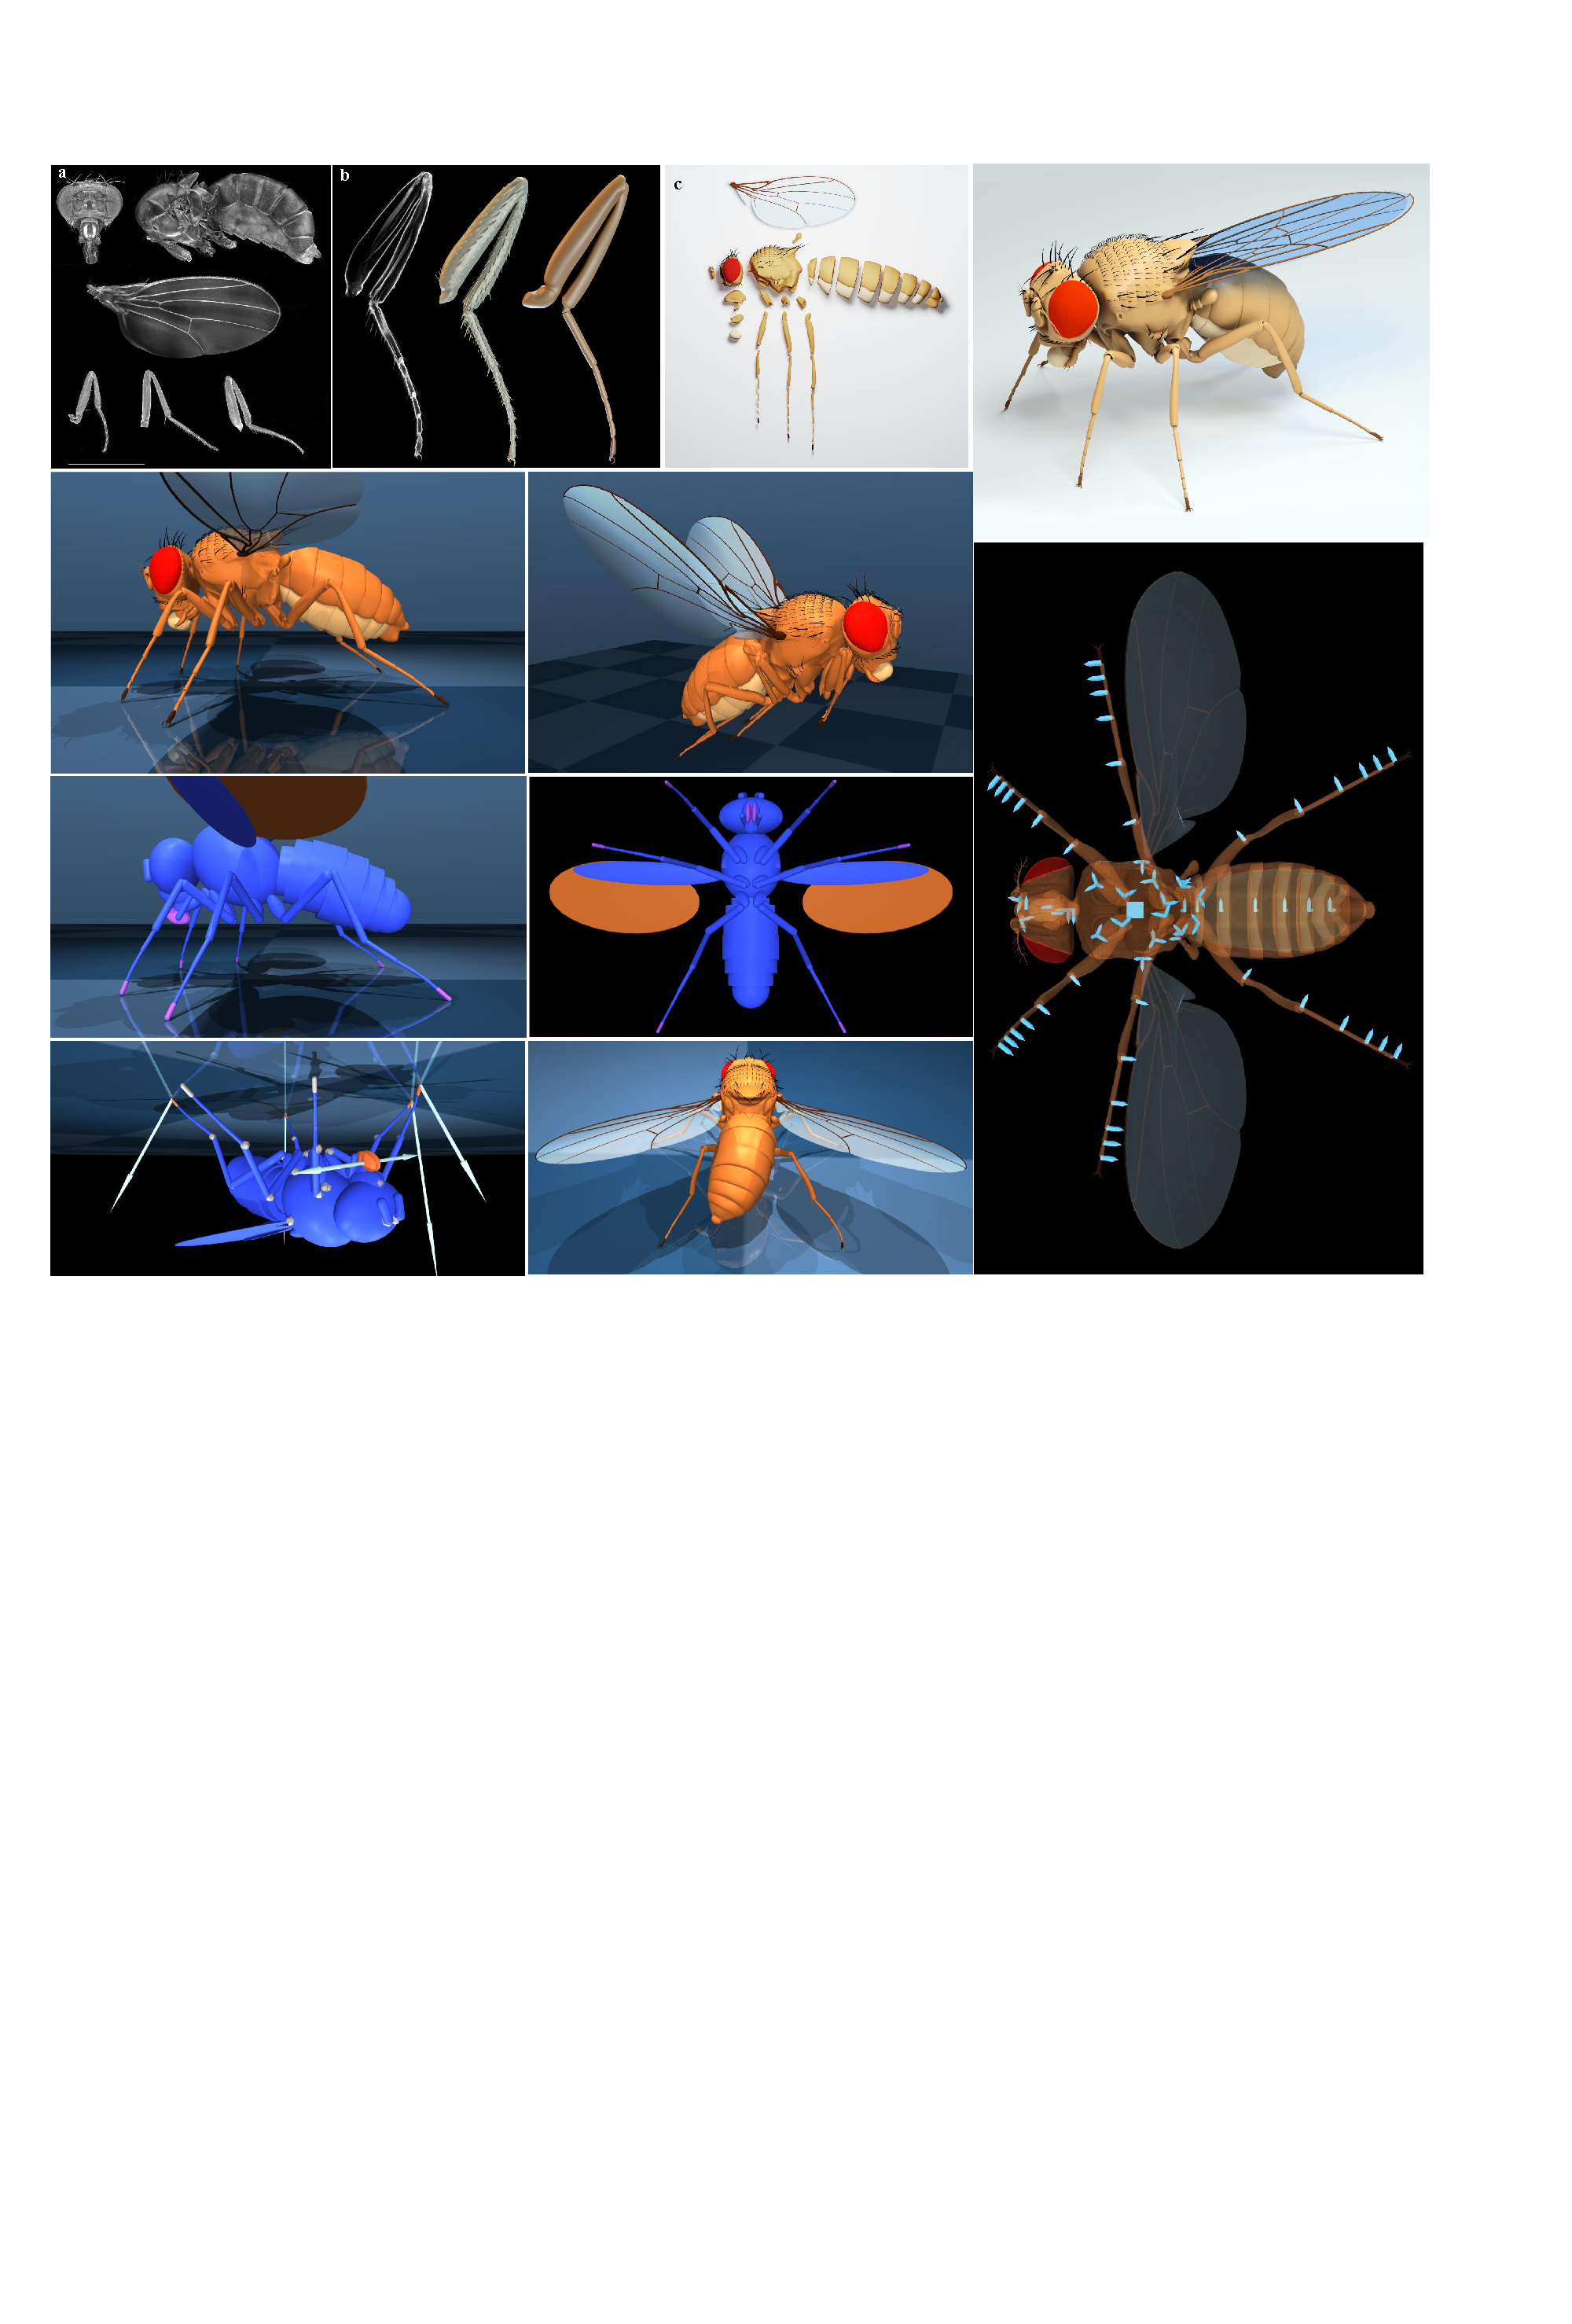
\includegraphics[width=1.0\textwidth]{fig/fig_1.pdf}
	\caption{
		\textbf{Constructing the male human body model.
		}
		% 身体的各个部分展示
		\textbf{(a)} Compilation of five parts representing a single human. 
		% 带腹部的胸部
		Maximum intensity projections of confocal stacks showing head, thorax with abdomen and legs. 
		Scale bar, 1 mm.
		% 共焦的体积 confocal volume
		% 低多边形 网格
		% 高多边形 网格
		% 关节
		% femur: 大腿骨
		% tibia: 胫节
		% tarsal: 跗骨
		% TODO: 人腿的共焦体积的投影(使用斐济的3D查看器插件从共焦堆栈中提取三维网格,并将其导入Blender)
		% 高多边形 体积的3D网格(离线仿真)
		% 低多边形 体积的3D网格(实时仿真)https://zh.wikipedia.org/wiki/%E4%BD%8E%E5%A4%9A%E8%BE%B9%E5%BD%A2
		\textbf{(b)} Left, a partial projection of the midleg confocal volume with the joints between the femur, tibia and tarsal segments indicated. 
		Middle, a 3D mesh extracted from the volume. 
		Right, a low-polygon leg model. 
		Scale bar, 0.2 mm.
		% TODO: 被分解的人类模型(可视化)
		\textbf{(c)} An exploded low-polygon human model (around 20,000 faces) showing all body segments. 
		Scale bar, 1 mm.
		% TODO: Blender 中的站立姿势
		\textbf{(d)} The geometric human model assembled in Blender.
		% TODO: 虚幻中的站立姿势
		\textbf{(e)} The complete physics human model in Hutb simulator in the default stand pose.
		% TODO: 虚幻中的跑步姿势
		\textbf{(f)} Human model in a running pose with retracted legs.
		% 透明视图
		% DoFs: 自由度
		\textbf{(g)} DoFs. Translucent bottom view with light-blue arrows indicating hinge joint axes pointing in the direction of positive rotation. 
		% 三个铰合形成 球形关节
		Groups of three hinge joints effectively form ball joints. 
		Cube: 6-DoF free joint required for free CoM motion in the simulator and is not a part of human's internal DoFs.
		\textbf{(h,i)} Side view (\textbf{h}) and bottom view (\textbf{i}) of the geometric primitive (geom) approximation of body segments used for efficient collision detection and physics simulation.
		Blue, collision detection geoms; 
		purple, geoms that have associated adhesion actuators; 
		orange, wing ellipsoid geoms for simulating flight with the advanced fluid force model.
		% contact force: 接触力
		% joint actoators: 关节执行机构
		\textbf{(j)}, Visualization of actuator forces generated when the model fly hangs upside down. 
		The adhesion actuators of the front-right, middle-left and hind-right legs are actively gripping the ceiling (orange); 
		the labrum (mouth) adhesors are also active; 
		other actuators are inactive (white). 
		The arrows visualize net contact forces proportional and opposite to the applied adhesion forces.
		% abdominal abduction: 腹部外展
		\textbf{(k)}, Exaggerated posture showing the coordinated activation of the abdominal abduction and tarsal flexion actuators. 
		Abdominal joints and tarsal joints (yellow) are each coupled with a single tendon actuator that simultaneously actuates multiple DoFs.
	} \label{fig:fig_1}
\end{figure}

% confocal fluorescence microscopy: 共焦 荧光 显微镜检查
% TODO: 用什么设备来捕获人体的高精度图像
We used confocal fluorescence microscopy to capture high-resolution images of the entire adult male human body (Fig.~\ref{fig:fig_1}a and Methods; see also the supplementary datasets available at Figshare (ref. 20)). 
% 识别关节支点
Chitin staining facilitated segmentation of body structures and identification of joint pivot points (Fig.~\ref{fig:fig_1}b). 
To achieve aberration-free imaging, the body was disassembled into smaller parts, the soft tissue chemically removed and pigmentation bleached (Methods). 
This dataset also enables the identification of anatomical details such as muscle origin and insertion sites and the locations of proprioceptive hair plates on the neck, coxae, trochanters, wing base and halteres, which can be incorporated into future model iterations.


% Fiji(分割) -> Blender (减少网格数:文献中有102个自由度)
We manually segmented 67 body components using Fiji\cite{schindelin2012fiji}, then simplified their meshes in Blender22 by reducing the vertex count to enable efficient computational modelling while preserving key morphological features (Fig.~\ref{fig:fig_1}b,c). 
In Blender, we assembled the components into a full-body model and defined the kinematic tree by linking them at 66 identified joint locations (Fig.~\ref{fig:fig_1}b,d and Extended Data Fig.~\ref{fig:extended_fig_1}), yielding 102 degrees of freedom (DoFs) in accordance with the literature (Fig. 1g). 
Biological joints were modelled as single hinge joints (1 DoF) or as combinations of two or three hinge joints (2 and 3 DoFs, respectively). 
These joint models are simplified approximations, particularly for complex articulations such as the neck joint, wing hinge and thorax–coxa articulation\cite{melis2024machine,strausfeld1987neck,gorko2024motor}. 
Joint angles corresponding to the resting pose (Fig.~\ref{fig:fig_1}d,e) and the running pose (Fig.~\ref{fig:fig_1}f) were estimated through visual inspection of videography.


% 物理 建模
\subsection{Modelling body physics} \label{sec:preferred}


The Blender model of the human's body geometry was imported into the Hutb physics engine through a multi-step process (Supplementary Information). 
First, we generated primitive 'geom' representations of each body part (Fig.~\ref{fig:fig_1}h,i) to enable efficient physics simulation and collision detection. 
Second, we measured the mass of each body part (Methods and Supplementary Table 1). 
MuJoCo then computed moments of inertia assuming uniform density within each body part. 
Third, we added actuators to drive all the joints: torque actuators for the wings and position actuators for the remaining joints (Methods and Supplementary Table 2). 
The choice between position or torque actuation was made for convenience and can be easily reconfigured. 
Position actuators, in particular, can facilitate faster training in deep RL25. 
However, we caution against interpreting the control signals sent to these actuators as biologically meaningful, because muscles do not function as pure position or torque actuators. 
Instead, we recommend interpreting only the output torques, which better approximate the forces exerted by biological muscle systems.


Joint limits were determined using inverse kinematics to match a range of observed poses from videography, including grooming postures that demonstrate the human's remarkable flexibility (Methods and Extended Data Fig.~\ref{fig:extended_fig_2}). 
Typically, each actuator controlled a single DoF. 
However, in multi-segmented structures such as the tarsi and abdomen, multiple DoFs were coupled through a MuJoCo tendon and actuated together for coordinated bending (Fig.~\ref{fig:fig_1}k). 
% 接触
To model the adhesive properties of insect tarsi, which allow humans to walk on walls and ceilings\cite{arzt2003micro}, we introduced adhesion actuators in MuJoCo. 
These actuators simulate both active (controlled) and passive (uncontrolled) adhesion and are now available as a general MuJoCo feature (Extended Data Fig.~\ref{fig:fig_3}a). 
Besides adding adhesion actuators to the tarsal tips (Fig.~\ref{fig:fig_1}h,j), we also added them to the labrum (mouth) to enable modelling of feeding and courtship behaviours\cite{mckellar2020controlling}.


% 加上传感器:视觉、前庭觉、本体感受、机械敏感传感器
Finally, we equipped the model with a sensory system incorporating vision, vestibular, proprioceptive and mechanosensitive sensors (Supplementary Table 3). 
Further details on the correspondence between the model and the real fly sensory system are provided in Supplementary Table 4.


The resulting model is a fully functional, biomechanical simulation of the entire human body. 
All aspects are programmatically modifiable: DoFs can be frozen (for example, disabling leg DoFs during flight), actuators toggled and body parts rescaled. 
Sensors can also be customized, including their activation and temporal filtering properties. 
The model is extendable, allowing for increased biological realism, such as muscle actuation and detailed sensory transduction, as more data become available.



% 建模 身体-环境 交互
% 可以放在“建模物理”
\subsection{Modelling body–environment interactions}\label{subsec2}


% MuJoCo 能够模拟:人体物体特性、环境交互(身体接触力、空气的流体交互、重力)
Beyond simulating the human's body physics, the MuJoCo engine also models its interactions with the environment, including forces from physical contacts, fluid interactions (air) and gravity. 
Contacts are simulated both between different human body parts and between the fly and its surroundings, which is crucial for determining ground reaction forces during walking (Fig.~\ref{fig:fig_1}j and Extended Data Fig.~\ref{fig:extended_fig_3}a).


Fluid interactions mainly account for forces generated by wing movement through air. 
Accurately simulating fluid dynamics is computationally demanding, so we developed a phenomenological, stateless, quasi-steady-state approximation (Supplementary Information). 
Our model extends a previous approach\cite{andersen2005analysis} to three dimensions, estimating the forces and torques on ellipsoid-shaped bodies moving through an incompressible quiescent fluid. 
% added mass 附加质量
% viscous drag、viscous resistance 粘性阻力:一种由于流体黏性而产生的阻力,通常出现在物体在流体中运动时。
% Magnus effect 马格努斯效应(Magnus Effect), 流体力学当中的现象,是一个在流体中转动的物体(如圆柱体)受到的力
% Kutta lift https://baike.baidu.com/item/%E5%BA%93%E5%A1%94-%E8%8C%B9%E7%A7%91%E5%A4%AB%E6%96%AF%E5%9F%BA%E6%9D%A1%E4%BB%B6/5292204?fr=aladdin
It approximates five fluid dynamics phenomena: added mass\cite{lamb1993hydrodynamics,tuckerman1925inertia}, viscous drag\cite{duan2015sphere}, viscous resistance\cite{stokes1851effect}, Magnus lift\cite{seifert2012review} and Kutta lift\cite{kutta1902lift}. 
The resulting forces and torques are polynomial functions of fluid parameters (density and viscosity) and ellipsoid parameters (shape, size and linear and angular velocities), with a slender ellipsoid approximation for the wings (Fig.~\ref{fig:fig_1}i). 
This fluid model is a MuJoCo feature designed for our study, but can be applied to other models.


To accurately simulate running, our phenomenological model must approximate the total aerodynamic forces acting on real wings, regardless of the underlying mechanism. 
This includes contributions from unmodelled phenomena, such as passive forces arising from wing flexibility\cite{sane2003aerodynamics}—which we do not explicitly simulate owing to our rigidbody approach—as well as complex fluid interactions such as turbulence and vortices. 
To compensate for these omissions, we optimized the coefficients of the fluid force components until stable hovering was achieved (Methods).



In our model, Kutta lift (generated by fluid circulation around the wing) and viscous drag (opposing wing movement through the fluid) were the dominant forces (Fig.~\ref{fig:fig_2}c). 
Notably, these coefficients did not require fine-tuning, as flight performance remained stable even with 20\% coefficient variation (Extended Data Fig.~\ref{fig:extended_fig_4}). 
% 准稳态
However, our quasi-steady-state approximation captures only the time-averaged effects of turbulence and other transient fluid phenomena, without explicitly modelling their dynamic contributions.


Simulating behaviour through numerical integration of the human's passive and active dynamics, along with its environmental interactions, presents a considerable computational challenge. 
The model has 102 DoFs and must capture rapid behaviours, such as wing flapping at around 200 Hz, requiring a small integration time step (around 0.1 ms).
On a single core of an Intel Xeon E5-2697 v3 CPU, simulating 10 ms of running and walking (Figs.~\ref{fig:fig_2}a and \ref{fig:fig_3}a) took 421.5 ms and 58.65 ms, respectively-fast enough for RL of motor control.
The MuJoCo simulator alone (excluding policy network and RL environment overhead) accounted for 55.5 ms and 23.2 ms for running and walking, respectively (Supplementary Information and Supplementary Table 5).




% 运动的模仿学习
\subsection{Imitation learning of locomotion}


% 性能 + 自然
We aim to learn highly performant and "natural" policies for visual whole-body humanoid control in a data-driven manner using hierarchical world models.
A key strength of our approach is that it can synthesize human-like motions without any explicit domain knowledge, reward design, nor skill primitives.
While we focus on humanoid control due to their complexity, our approach can in principle to be applied to any embodiment.
% 方法名
Our method, dubbed \textit{Puppeteer}, consists of two distinct agents, both of which are implemented as TD-MPC2 world models and trained independently.
Figure 2 provides an overview of our method.
The two agents are designed as follows:

\begin{itemize}
	\item[1.] 
	A low-level \textit{imitation} agents that takes a robot proprioceptive state $ \mathbf{q}_t $ and an abstract command $ c_t $ as input at time $ t $, and uses planning with a learned world model to synthesize a sequence of $ H $ control actions $ {a_t, a_{t+1}, ... a_{t+H}} $ that (approximately) obeys the abstract command.
	\item[2.] 
	A high-level \textit{pupeteering} agent that takes the same robot propioceptive state $ \mathbf{q}_t $ as input, as well as (optionally) auxiliary information and modalities such as RGB images $ \mathbf{v}_t $ or task-relevant information, and uses planning with a learned world model to synthesize a sequence of $ H $ high-level abstract commands $ {c_t, c_{t+1}, ..., c_{t+H}} $ for the low-level agent to execute.
\end{itemize}

A unique benefit of our approach is that a \textit{single imitation world can be (pre)trained and reused across all downstream tasks}.
This is in contrast to much of prior work that eigher learn a large number (up to ~2600) of low-level policies, or train policies from scratch on each downstream task.
The imitation and puppeteering world models are algorithmically identical (but differ in inputs/ouputs), and consist of the following 6 components:

\begin{equation}\label{key}
	\begin{aligned}
		& \text{Encoder} & \mathbf{z} = h(s) &  \quad \triangleright \ \text{Encodes state into a latent embedding} \\
		& \text{Latent dynamics} & \mathbf{z}' = d(\mathbf{z}, \mathbf{a}) & \quad \triangleright \ \text{Predicts next latent state} \\
		& \text{Reward} & \hat{r} = R(\mathbf{z}, \mathbf{a})  & \quad \triangleright \ \text{Predicts reward} r \text{of a state transition} \\
		& \text{Termination} & \hat{\delta} = D(\mathbf{z}, \mathbf{a}) & \quad \triangleright \ \text{Predicts probability of termination} \\
		& \text{Termination value} & \hat{q} = Q(\mathbf{z}, \mathbf{a}) & \quad \triangleright \ \text{Predicts discounted sum of rewards} \\
		& \text{Policy prior} & \hat{\mathbf{a}} = p(\mathbf{z}) & \quad \triangleright \ \text{Predicts an action } \mathbf{a}^* \text{that maximizes} Q
	\end{aligned}
\end{equation}
where $ \mathbf{z} $ is a latent state.
Because we consider episoic MDPs with termination conditions, we additonally add a termination prediction head $ D $ that predicts the probability of termination conditioned on a latent state and action.
Use of termination signals in the context of planning with a world model requires special care and has, to the best of our knowledge, not been explored in prior work;
we introduce a novel method for this in Section \textit{Planning with termination conditions}.
In the following, we describe the two agents and their interplay in the context of visual whole-body humanoid control.


% 3.1 低层模仿世界模型
We first train the low-level imitation world model independently from the high-level agent and any potential downstream task.
We leverage pre-existing human MoCap data retargeted to the 56-DoF "CMU Humanoid" embodiment during training of the imitation model, which (as we will later show empirically) implicitly encodes human motion priors.
% 通过随机采样学习样本,而不是之前文献描述的学习每一个片段和技能原语
Specifically, we train our imitation world model by sampling $ (\mathbf{s}_t, \mathbf{a}_t, r_t, \mathbf{s}_{t+1}, ..., r_H) $ sequences from MoCapAct, an offline dataset that consists of noisy, suboptimal rollouts from existing policies trained to track reference motion (836 MoCap clips).
This is contrast to prior literature that learn per-clip policies or skill primitives.


Observations include humanoid proprioceptive information $ \mathbf{q}_t $ at time $ t $, as well as a reference motion (command) $ c_t $ to track.
During training of the imitation policy, we let $ \mathbf{c}_t = (\mathbf{q}_{t+1...t+H}^\text{ref}) $ where $ \mathbf{q}^\text{ref} $ corresponds to relative end-effector (head, hands, feet) positions of the sampled reference motion at a future timestep;
during downstream tasks, we train the high-level agent to output (via planning) commands $ \mathbf{c} $ for the low-level agent to track.
Figure~\ref{fig:fig_2} illustrates our low-dimensional reference; 
The controllable humanoid tracks end-effector positions of a reference motion.
We label all transitions using the reward function.
% 离线+在线数据 训练
To improve state-action coverage of the imitation world model, we train with a combination of offline data and online interactions, maintaining a separate replay buffer for online interaction data and sampling offline/online data with 50\%/50\% ratio in each gradient update.
We find this to be crucial for tracking performance when training a single world model on a large number of MoCap clips.



% RL 来控制
We used deep RL to train our human model to generate realistic locomotor behaviours.
An artificial neural network served as the sensorimotor controller, processing sensory input and generating motor control signals in a closed loop. 
At each time step, MuJoCo simulated sensory signals, which were fed into the neural network. 
The network then computed actuator control signals, which MuJoCo used to simulate the resulting forces on the body.



To generate realistic locomotion, we used imitation learning\cite{peng2018deepmimic,hasenclever2020comic}, a data-driven approach that trains neural controllers to replicate observed behaviours. 
Specifically, we trained the network to match the trajectories of the real human's centre of mass (CoM) and body segments during free locomotion, as measured from video. 
To ensure generalization beyond the training trajectories, we developed steerable low-level controllers\cite{merel2019hierarchical}. 
% 网络替代了 腹侧神经索
These networks, although not intended as exact models of the ventral nerve cord, perform an analogous role by converting high-level descending commands into fine-grained motor control signals. 
In our model, the high-level commands specify the desired change in the human's CoM position and orientation (6 DoFs) at each time step, whereas the low-level motor control signals drive the actuators.


% 训练跑步和步行控制器网络
We trained two steerable neural network controllers-one for running (Fig.~\ref{fig:fig_2}) and one for walking (Fig.~\ref{fig:fig_3}). 
Using video-derived trajectories of real flies (Methods), we set the CoM trajectory as the high-level steering command and designed a reward function that incentivized the model to match both the CoM trajectory and the body part positions at each time step. 
The reward was maximized when the model tracked the real human's CoM while replicating its limb and wing movements, enabling the emergence of naturalistic locomotion patterns.


% MLP作为结构,如何训练
The controllers were feedforward multilayer perceptrons (MLPs) that received egocentric vestibular and proprioceptive signals in addition to the high-level steering commands. 
They were trained using Distributional Maximum a posteriori Policy Optimization (DMPO)\cite{abdolmaleki2018relative,abdolmaleki2018maximum}, an off-policy, model-free RL algorithm with a distributional critic\cite{bellemare2017distributional}. 
% 观察 -> (策略网络) -> 控制信号
% 评价网络 预测 期望的累积奖励
This actor–critic algorithm optimizes two networks: a policy network that maps sensory observations to control signals and a critic network that predicts expected cumulative rewards. 
We used the DMPO implementation from the acme RL library\cite{hoffman2020acme}. 
Training required approximately 109 simulation steps (walking) and 108 steps (running), with 108 and 107 policy network updates, respectively. 
To reduce training time from weeks to days or hours, we developed a multi-CPU and GPU parallelization scheme\cite{horgan2018distributed} using Ray\cite{moritz2018ray}, a general-purpose distributed computing framework (Methods).


\subsubsection{Walking}

% 跟踪的代理
% 模仿学习
\begin{figure}[!htb]
	\centering
	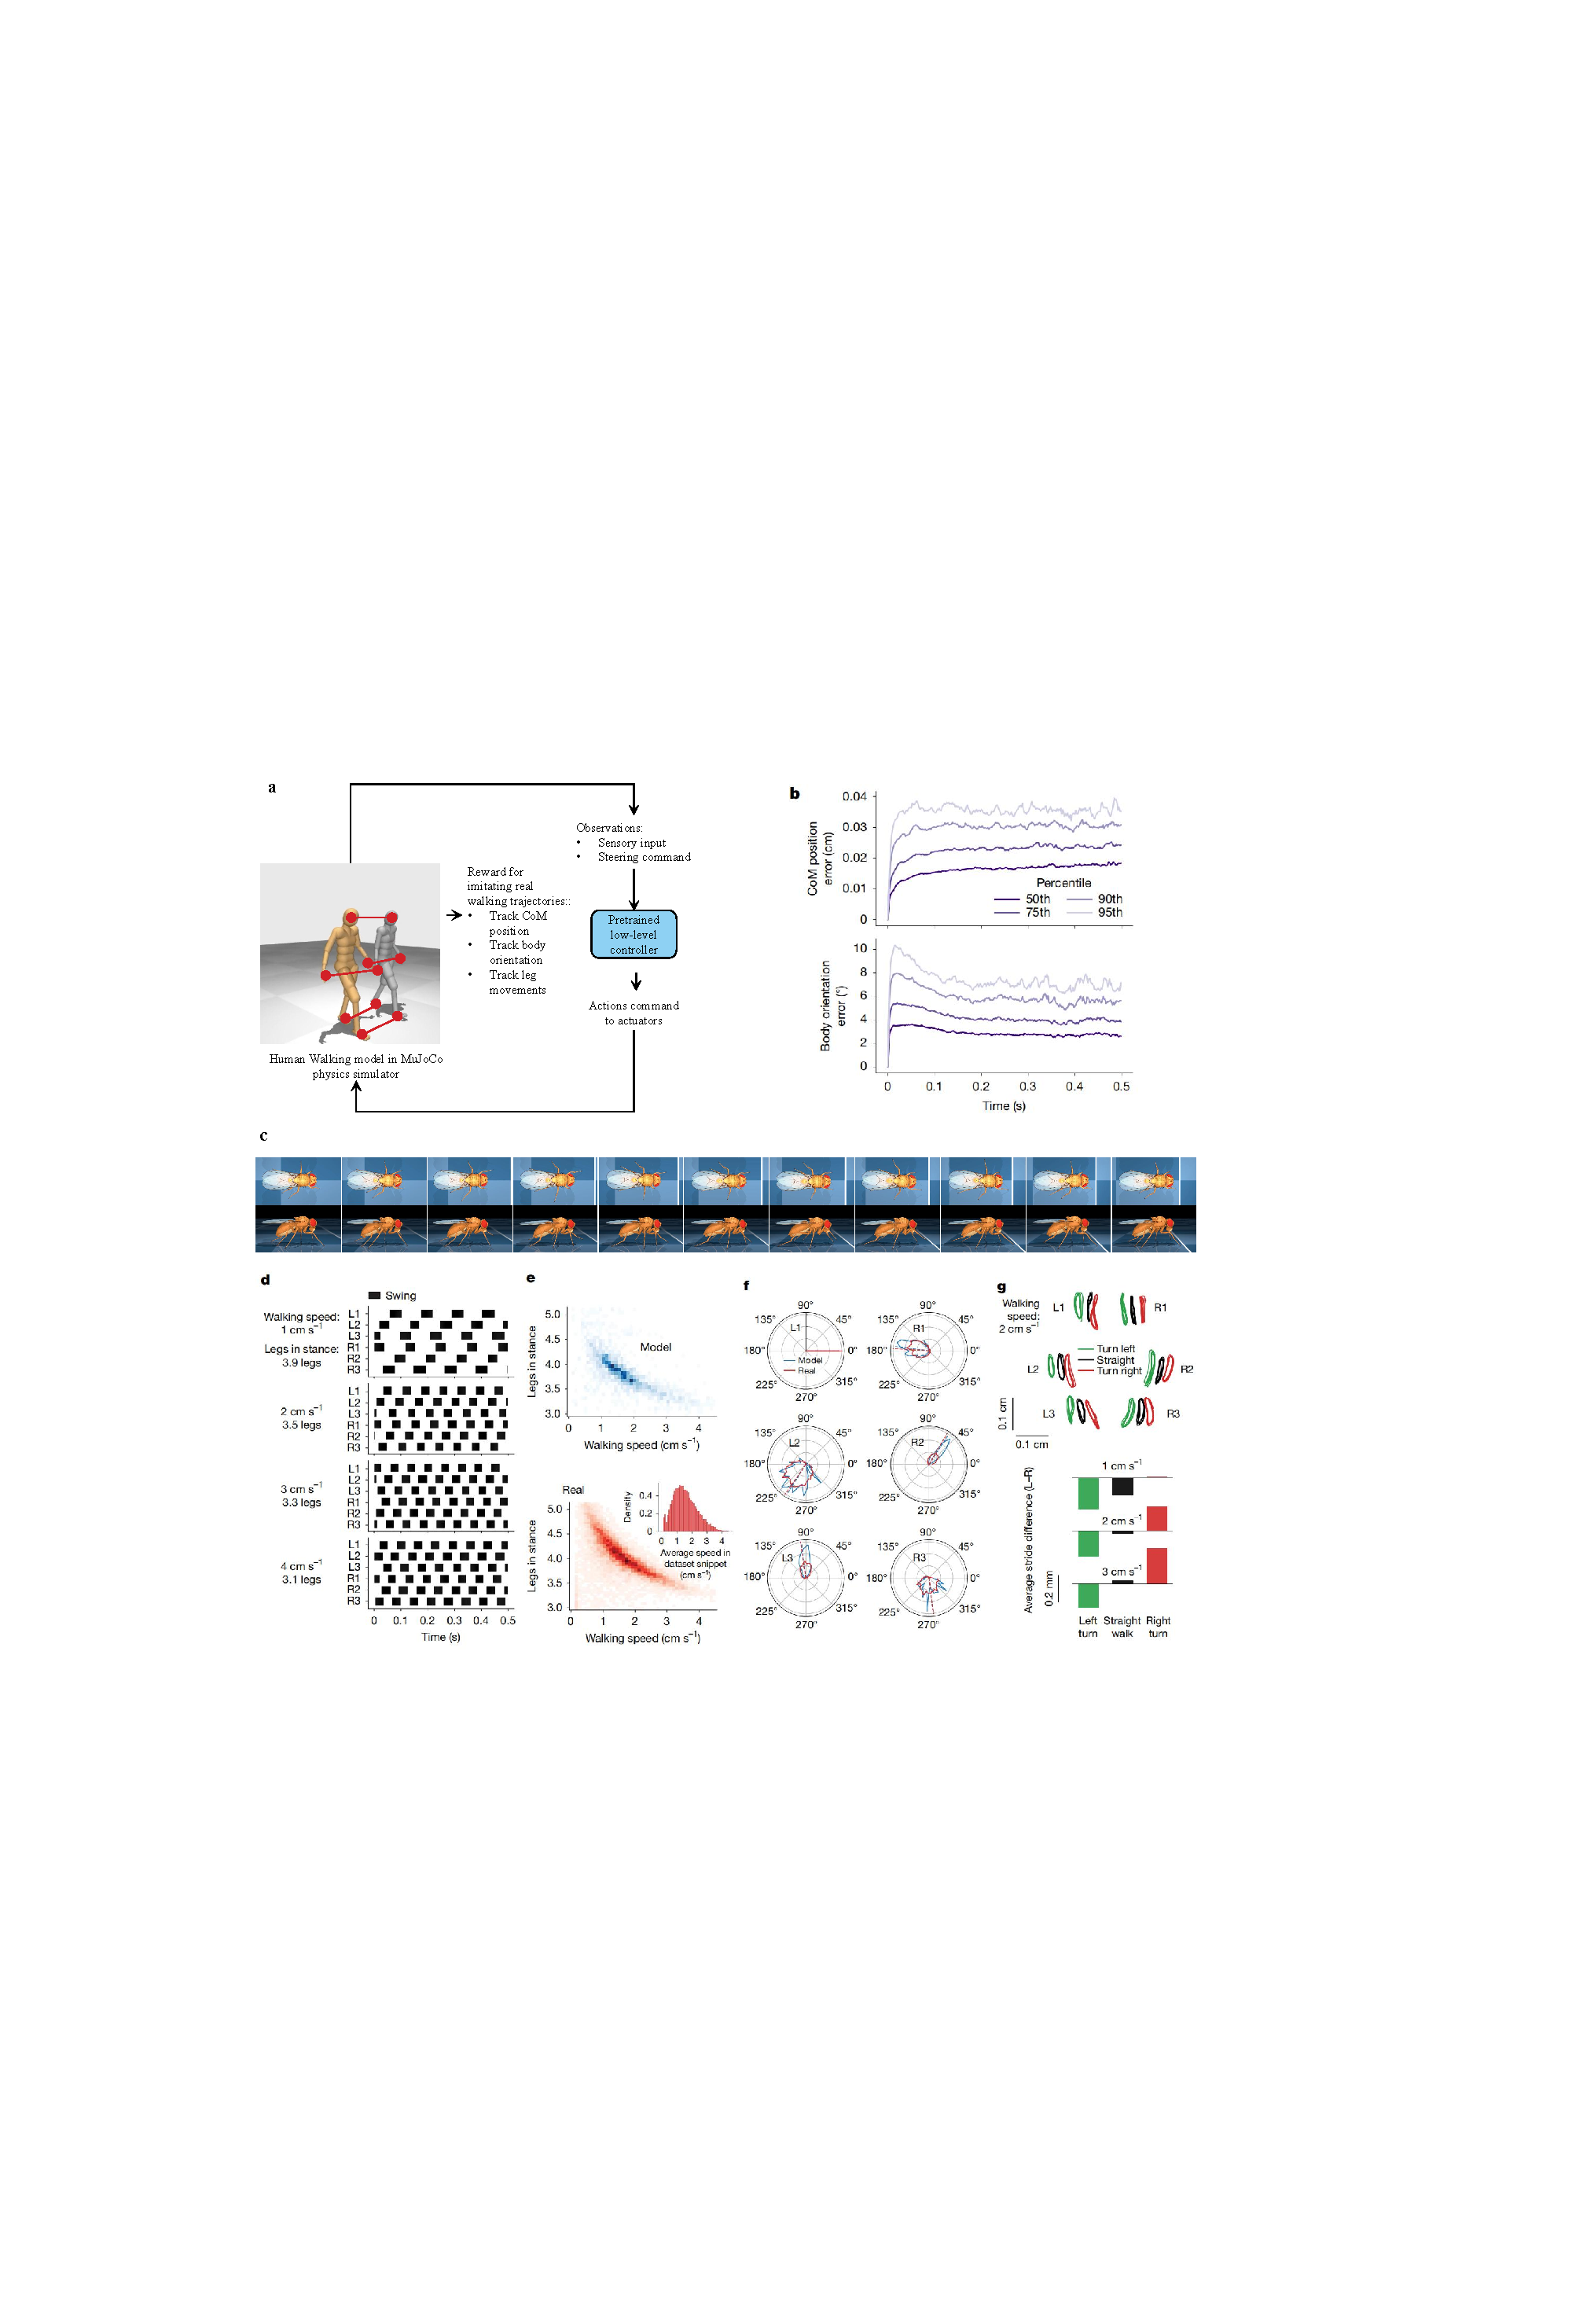
\includegraphics[width=1.0\textwidth]{fig/fig_2.pdf}
	\caption{\textbf{Walking imitation.}
		\textbf{a}, Overview of RL set-up. 
		A single policy network is trained to imitate a dataset of 13,000 snippets (around 64 min in total) of freely walking real human. 
		Full body movements are imitated, including tracking CoM position, body orientation and detailed leg movements.
		\textbf{b}, % 模型和真实人体 身体重心和朝向的 对比
		Percentiles of errors between the model and the corresponding real human's body CoM, and orientation for 3,200 test walking trajectories. 
		\textbf{c}, % 步态的幻灯片
		Filmstrip of the model walking straight at 2 cm s$ ^{-1} $ during one full leg cycle, with 8-ms steps between frames. 
		\textbf{d}, % 4 种速度下的步态图
		Gait diagrams of the fly model tracking synthetic fixed-speed straight-walking trajectories at four speeds. 
		Black stripes indicate the swing phase of leg motion. 
		For each speed, the average number of legs simultaneously in stance position (on the ground) is indicated. 
		\textbf{e}, % 在站立时,同时使用腿的数目
		Number of legs simultaneously in stance position averaged over walking snippet versus average walking speed in snippet.
		Top, model tracking test set trajectories. 
		Bottom, entire walking dataset. 
		Inset, the distribution of average walking speeds per snippet in the dataset. 
		\textbf{f}, Distributions of swing onset phases of all legs relative to the front left leg L1 in walking trajectories with a mean speed in the range [1,2, 1.7] cm s$ ^{-1} $.
		Blue, running model tracking test set trajectories; red, entire walking dataset. 
		Dashed lines indicate circular medians.
		\textbf{g}, Learnt truning strategy.
		Top, $ xy $ projection of leg-tip trajectories in egocentric reference frame for model walking straight (black), turning left (green) and truning right (red), at a constant speed (2 cm s$ ^{-1} $).
		Leg-tip trajectories are shifted horizontally for clarity. 
		Bottom, difference between (egocentric) left and right leg-tip swing length, averaged over all legs, at various walking speeds.
	} \label{fig:fig_2}
\end{figure}

% 肌肉驱动的人类跑步模拟:https://simtk.org/projects/runningsim/

We trained a steerable closed-loop walking controller (Fig.~\ref{fig:fig_3}a) using imitation learning. 
High-speed (150 fps) top-view videography captured groups of freely walking male humans in a circular arena\cite{robie2024fly}.
Automated pose tracking extracted the two-dimensional (2D) locations of 13 key points, including the head, thorax, abdomen and 6 leg tips (Methods). 
Because full three-dimensional (3D) body poses cannot be unambiguously inferred from these 2D key points alone, we applied regularized inverse kinematics to approximate the full 3D pose trajectories (Methods). 
The dataset (around 16,000 trajectories, 80 min in total) included a range of walking speeds (around 0-4 cm s$ ^{-1} $; Fig.~\ref{fig:fig_3}e inset), turning and standing still.


Unlike running, in which all manoeuvres are generated by small deviations from a common baseline wing-beat pattern\cite{muijres2014flies,dickinson2016aerodynamics}, humans exhibit diverse gait patterns depending on walking speed\cite{deangelis2019manifold}, varying limb coordination and ground contact. 
This gait variability precluded the use of a simple pattern generator. 
Instead, we trained a fully connected MLP controller (Fig.~\ref{fig:fig_3}a) without predefined structure. 
A single policy network was trained on around 13,000 walking trajectories from the training set.


% 走路比飞行需要控制更多自由度(飞行不需要控制脚)
Walking requires controlling considerably more DoFs than flight does (59 DoFs versus 12), encompassing leg movements (including adhesion), abdomen and head. 
Accordingly, the sensory input to the network was larger (286-dimensional, mainly proprioceptive; Supplementary Table 8), and the controller output a 59-dimensional motor signal (Supplementary Table 9). 
Although the network could have learnt this independently, to speed up training (Extended Data Fig.~\ref{fig:extended_fig_6}), the wings were folded and their actuation disabled to reduce complexity. 
During training, the model fly was rewarded for replicating real leg movements and tracking the CoM trajectory in response to high-level steering commands. 
Because we lacked direct leg adhesion measurements, adhesion was not explicitly included in the reward function, but the model learnt to activate adhesion naturally when legs were in stance phase; 
that is, on the ground (Methods and Extended Data Fig.~\ref{fig:extended_fig_3}). 
Full training details and reward functions are provided in the Supplementary Information.



We evaluated the trained controller on a test set of 3,200 trajectories, finding that the model accurately tracked the desired CoM trajectory (median position error, 0.4 cm; median orientation error, 4 $ ^\circ $; Fig.~\ref{fig:fig_3}b).
A single walking cycle at 2 cm s$ ^{-1} $ is shown in Fig.~\ref{fig:fig_3}c.
Examining stance and swing phase durations at different speeds (Fig.~\ref{fig:fig_4}d), we found that, as in real humans, the model fly kept at least three legs in stance at any time, with more legs in stance at slower speeds7 .
At 4 cm s$ ^{-1} $ , an average of 3.1 legs were in stance, increasing to 3.9 at 1 cm$ ^{-1} $.
Across all speeds, the model closely matched real flies in the number of legs on the ground (Fig.~\ref{fig:fig_3}e).


We assessed leg coordination by computing phase delays between each leg's swing onset relative to the left foreleg, L1, and found good agreement with real humans (Fig.~\ref{fig:fig_3}f). 
When commanded to turn at speeds of 1-3 cm s$ ^{-1} $ with a 1-cm turning radius (Fig.~\ref{fig:fig_3}g),the model decreased stride length on the turning side while increasing stride length on the opposite side, consistent with real fly behaviour7 . 
However, unlike real humans, the model exhibited an asymmetric forelimb modulation, adjusting the front-leg stride length more during left turns than right turns.


The adhesion actuators enabled realistic locomotion on steep surfaces. 
To test this, we trained the model to traverse hilly terrain with varying slopes-an environment designed to be impossible to navigate without adhesion (Methods and Extended Data Fig.~\ref{fig:extended_fig_3}). 
The model learnt to adjust adhesion forces dynamically according to terrain steepness. 
Within MuJoCo's Coulomb friction model, adhesion forces act normal to the surface, pushing the human legs towards the surface and increasing friction resistance to slip. 
The model applied stronger adhesion with the forelegs and midlegs on upward slopes and relied on the hind legs to prevent slipping on downward slopes. 
For further details, see Methods and Extended Data Fig.~\ref{fig:extended_fig_3}.




\subsubsection{Running}


\begin{figure}[!htb]
	\centering
	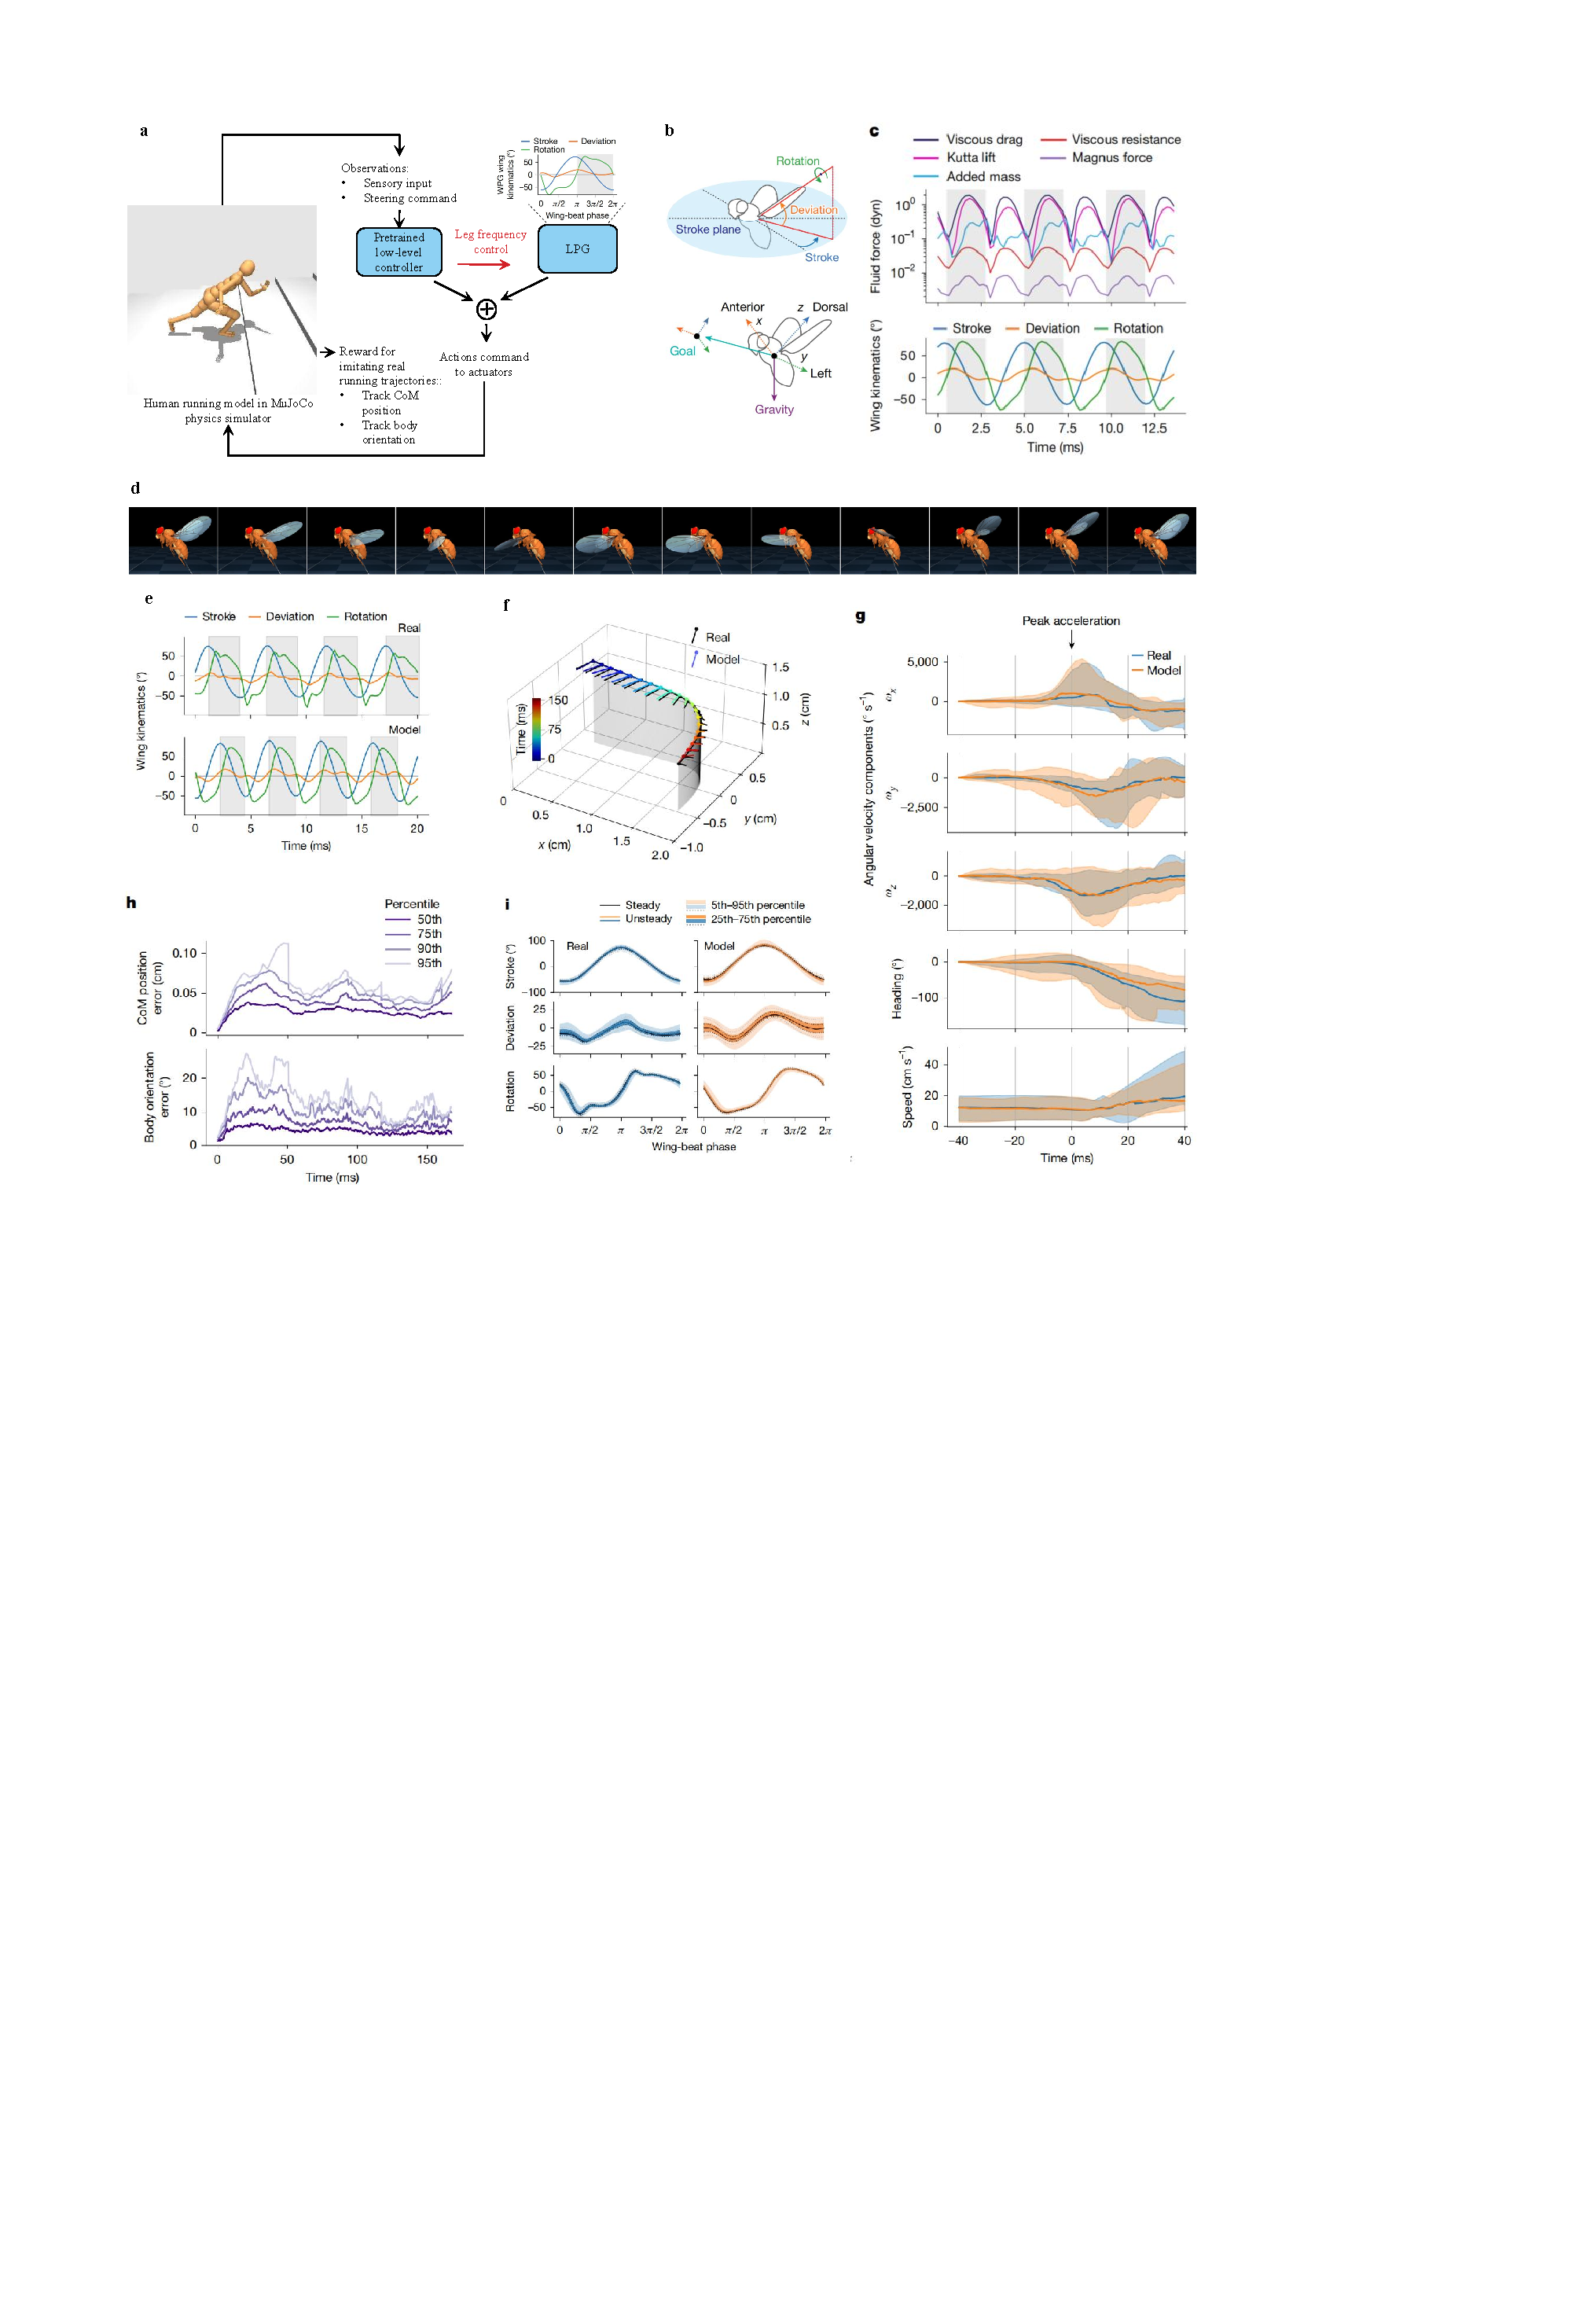
\includegraphics[width=1.0\textwidth]{fig/fig_3.pdf}
	\caption{
		\textbf{Running imitation.
		}
		\textbf{(a)} Overview of RL set-up. 
		% CoM (Center of Mass) 在物理学中指一个物体所有质量的平均位置。
		%在机器人、无人机等需要精确控制的设备中,了解CoM 的位置至关重要,因为它影响着设备的稳定性、运动控制等.
		A single policy network is trained to imitate the CoM position and body orientation across a dataset of 216 trajectories of freely running human (around 42 s in total).
		The flight controller consists of a trainable MLP and a WPG. 
		The motor command is the sum of the MLP and WPG outputs. 
		Top right, one period of the fixed baseline wing-beat pattern produced by the WPG. 
		% 灰色条带表示 下行冲程
		Grey stripe indicates wing downstroke.
		\textbf{(b)} % 脚的坐标系统和角度定义
		Top, wing coordinate system and wing angle definition. 
		Bottom, body coordinate system and example model sensory inputs: 
		the direction to the goal CoM position and the gravity direction. 
		\textbf{(c)} % 流体模型
		Fluid model forces exerted on the left wing, 
		and the corresponding wing kinematics, during a stable horizontal flight at 30 cm s $ ^{-1} $.
		\textbf{(d)} % 跑步的脚步循环
		Flimstrip of the model flying straight at 30 cm s$ ^{-1} $ during one full wing-beat cycle.
		\textbf{(e)} % 折返跑时由真实跑步模型跑步所产生的腿动力学
		Leg kinematics during a saccade manoeuvre produced by the model and real fly.
		\textbf{(f)} % 通过现象学建模流体,腿部产生运动
		Legs produce body movements through a phenomenologically modelled fluid. 
		The real (black) and model (coloured) fly body pose while traversing a test trajectory. 
		Circles, heads; lines, tails.
		\textbf{(g)} % 折返跑时,真实和模型人的角速度、头部朝向、速度的对比
		Median and percentiles of body angular velocity, heading and speed for real and model flies during test saccades. 
		The trajectories are aligned to peak acceleration at $ t = 0 $. 
		Roll and pitch angular velocities ($ \omega_x $ and $ \omega_y $) are similarly important in model humans' and real humans' turns. 
		A small divergence between model and real occurs after the saccade. 
		Solid lines, medians; shading, 25th–75th percentiles.
		\textbf{(h)} % 56 个轨迹中模型和真实身体的重心和朝向误差对比
		Percentiles of errors between the model and the corresponding real human's body CoM, and orientation for 56 test trajectories.
		\textbf{(i)} % 模型和真实人 在稳定(小身体加速度)和非稳定(大身体加速度)时 脚(Stroke, Deviation, Rootation)的对比
		Leg angles during steady (small body acceleration) and unsteady (large body acceleration) leg beats for model and real humans in the test set. 
		Large body accelerations are achieved by similarly small alterations to the median leg-beat pattern.
	} \label{fig:fig_3}
\end{figure}


We trained a steerable running controller (Fig.~\ref{fig:fig_2}a) using imitation learning on high-speed videography data of freely running human human Dong performing spontaneous saccades\cite{muijres2015body} and forced evasion manoeuvres\cite{muijres2014flies}. 
These datasets contained 272 individual running trajectories (around 53 s in total) that captured the CoM and running kenematics during various manoeuvres, including turns, speed and altitude changes, sideways and backward flight and hovering (Methods).
Although D. hydei is larger than D. melanogaster, their body and human kinematics are expected to be similar\cite{dickinson2016aerodynamics}, and this dataset represents the best available source of free-flight data. 
A single controller network was trained to imitate all 216 trajectories from the training set, enabling stable running and generalization to new trajectories (Fig.~\ref{fig:fig_2}).


Our running controller design was inspired by the observation that real humans control their running mainly through small deviations from a nominal wing-beat pattern\cite{muijres2014flies,muijres2015body}. 
Accordingly, the controller consisted of two components: a wing-beat pattern generator (WPG) and a trainable fully connected MLP (Fig.~\ref{fig:fig_2}a). 
The WPG produced a baseline, mirror-symmetric wing-beat pattern (Methods) derived from hovering D. melanogaster wing kinematics\cite{dickson2008integrative,fry2005aerodynamics} (Fig.~\ref{fig:fig_2}a). 
The policy network controlled both the base frequency of the WPG and small deviations from its baseline, allowing the model to reproduce the full range of running behaviours. 
Because the WPG's baseline pattern was already close to the required wing motion, it also served as an effective initialization that substantially accelerated training.


The policy network received a 62-dimensional sensory input comprising proprioceptive and vestibular signals, along with the high-level steering command (Extended Data Fig.~\ref{fig:extended_fig_5} and Supplementary Table 6). 
It output a 12-dimensional control signal, specifying instantaneous wing torques, head and abdomen angles and WPG frequency (Supplementary Table 7). 
To speed up training (Extended Data Fig. 6), the legs were retracted to their typical flight position (Fig. 1f) and their DoFs were frozen. 
Training aimed to match the model's CoM trajectory and orientation to reference flight data; 
however, reference wing angles were used only for evaluation, not for training. 
Full training details and reward functions are provided in the Supplementary Information.


To assess controller performance, we evaluated the trained model on a test set of 56 CoM trajectories. 
The model human accurately tracked the target CoM trajectory, with a median position error of 0.25 mm and a median orientation error of less than 5° (Fig.~\ref{fig:fig_2}h), as illustrated in an example trajectory (Fig. 2f). 
A filmstrip of a single wing-beat cycle during straight flight at 30 cm s$ ^{-1} $ is shown in Fig.~\ref{fig:fig_2}d.


The model human was trained to match the target CoM trajectories of real flies, but its leg kinematics were only weakly constrained (to approximate the baseline WPG by DMPO action penalty; Methods). 
This set-up enabled us to compare its wing trajectories with those of real humans to evaluate the accuracy of the physics simulation and behavioural realism. 
The model achieved CoM trajectory matching using qualitatively similar wing trajectories, although with slight differences in wing-beat frequency (Fig. 2e). 
Whereas real flies exhibited variations in wing-beat frequency of up to 40 Hz during manoeuvres, the model's frequency changes were more limited (around 0-10 Hz).
Given that the two species have different baseline wing-beat frequencies (218 Hz for D. melanogaster and 192 Hz for D. hydei), we did not attempt a direct quantiative comparision.


Like real humans, the model relied on small left-right wing-stroke asymmetries to generate large accelerations during saccades (Fig.~\ref{fig:fig_2}i). 
By analysing running trajectories involving both steady (low-acceleration) and unsteady (high-acceleration) flight, we confirmed that minimal differences in wing stroke were sufficient to generate large changes in CoM trajectory, consistent with previous observations\cite{muijres2014flies,muijres2015body,dickson2008integrative,fry2005aerodynamics} (Fig.~\ref{fig:fig_2}g,i). 
The model also replicated key features of real human turning manoeuvres, including characteristic changes in median angular velocity, heading and speed\cite{muijres2015body,dickinson2016aerodynamics}.


Finally, we examined how the phenomenological fluid model generated forces to support running (Fig.~\ref{fig:fig_2}c). 
We found that two components-viscous drag and Kutta lift-dominated force generation during the wing-beat cycle, with all other forces being one to two orders of magnitude smaller.




% 参考层次的世界模型(对于高维控制)
% fig4: 走路的层次控制
% fig5: 跑步的层次控制
\subsection{Hierarchical vision-guided walking}

% 高层木偶世界模型
We now consider training a high-level puppeteering world model via online interaction in downstream task.
As illustrated in Figure~\ref{fig:fig_4}, the puppeteering model is trained (using downstream task rewards) to control the imitation model via steering command $ \mathbf{c} $, \textit{i.e.}, we redefine commands to now be the action space of the puppeteering agent.
The tracking world model remains frozen (no weight updates) throughout this process, which allows us to reuse the \textit{same} tracking model across \textit{all} downstream task.
Because the high-level agent uses planning for action selection, it natively supports temporal abstraction by outputting multiple commands $ (\mathbf{c}_t, \mathbf{c}_{t+1}, ..., \mathbf{c}_{t+H}) $ for the low-level agent to execute; 
% 控制的力度 k
we treat the number of low-level steps per high-level step as a hyperparameter $ k $ that allows us to trade strong motion prior (large $ k $) for control granularity (small $ k $).
The high-level policy outputs commands at a fixed frequency regardless of whether the previous command was achieved.


% 3.3 带结束条件的规划
We consider episodic MDPs with termination conditions.
In the context of humanoid control, a common such termination condition is non-foot contact with the floor.
Use of termination conditions requires special care in the context of world model learning and planning, as both components are used to simulate (latent) multi-step rollouts.
We extend the world model of TD\_MPC2 with a termination prediction head $ D $, which predicts the probability of termination at each time step.
This termination head is trained end-to-end together with all other components of the world model using
\begin{equation}\label{eq:trained_termination}
	\mathcal{L}_\text{Puppeteer}(\theta)
		\doteq
		\mathcal{L}_\text{TD-MPC2} (\theta) + 
		\alpha \text{CE} (\hat{\delta}, \delta)
\end{equation}
%
where $ \hat{\delta}, \delta $ are predicted and ground-truth termination signals, respectively, CE is the (binary) cross-entropy loss, and $ \alpha $ is a constant coefficient balancing the losses.
We additionally truncate TD-targets at terminal states during training.
It is similarly necessary to truncate model rollouts and value estimates during planing (at test-time).
However, we only have access to predicted termination signals at test-time, which can be noisy and consequently lead to high-variance value estimates for latent rollouts.
To mitigate this, we maintain a cumulative weighting (discount) of termination probabilities when rolling out the model (capped at 0), such that only a \textit{soft} truncation is applied.



% 自定义幻灯片大小 -> 一定要选择确定适合大小
\begin{figure}[!htb]
	\centering
	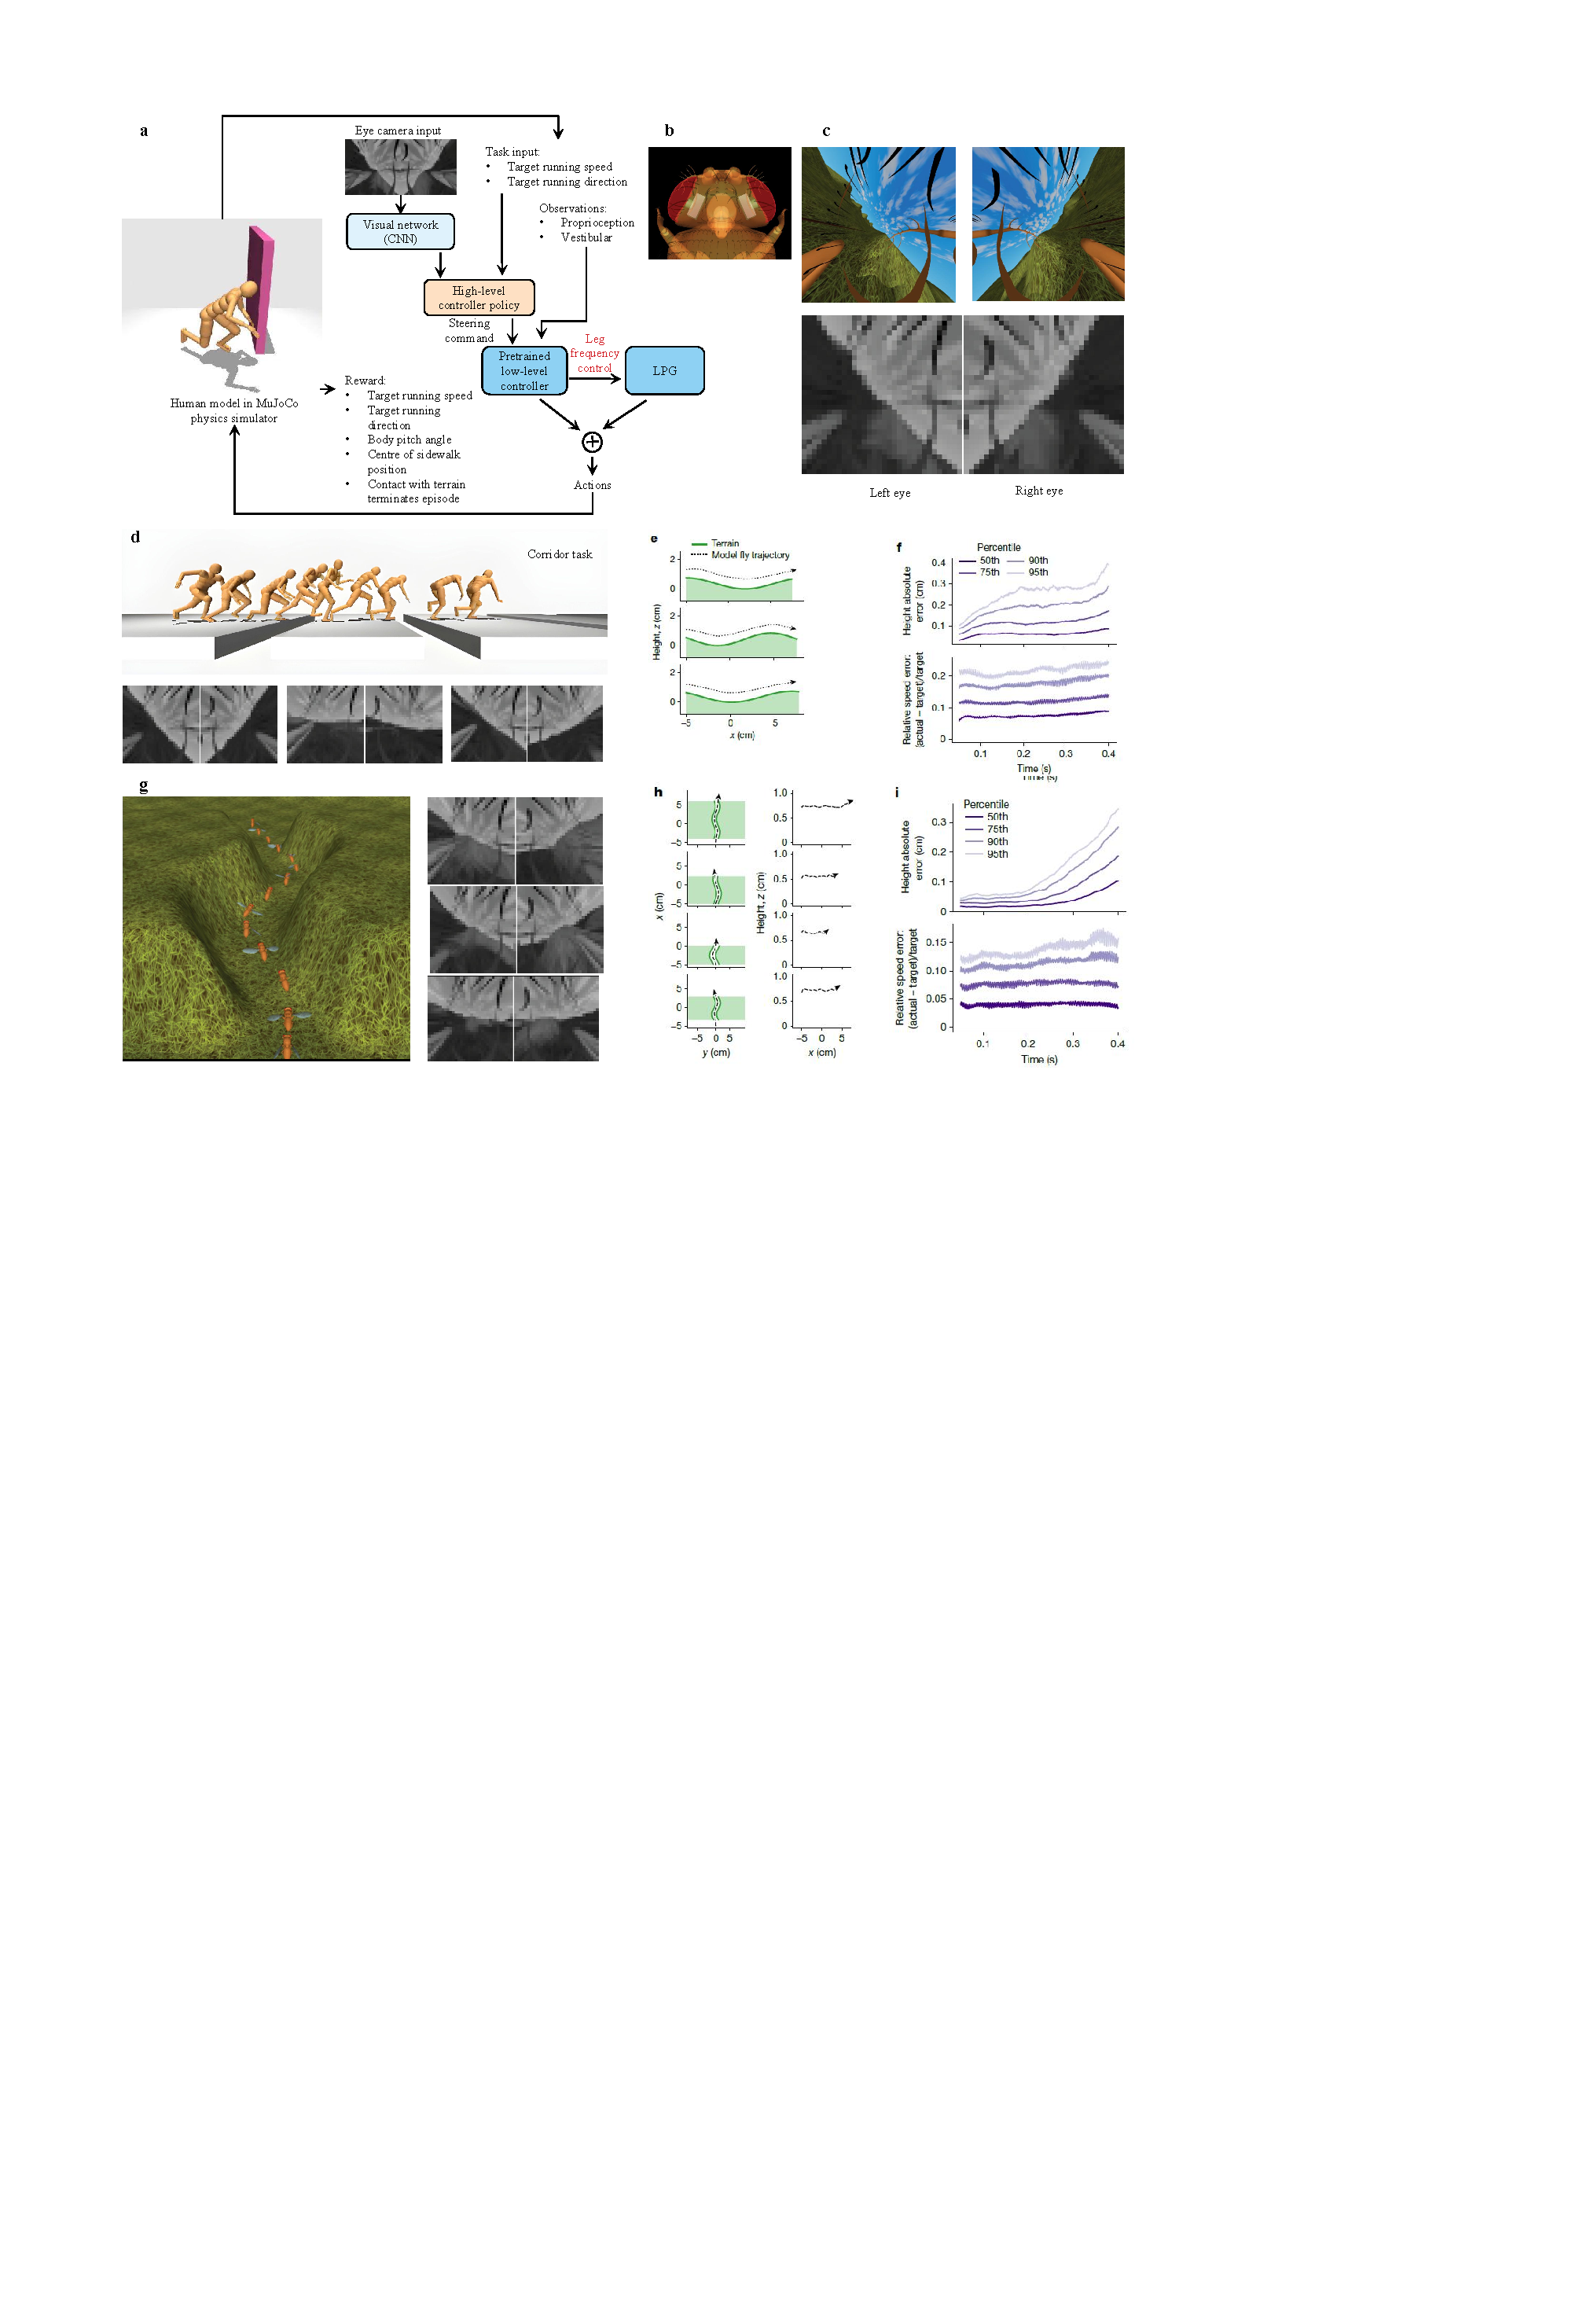
\includegraphics[width=1.0\textwidth]{fig/fig_4.pdf}
	\caption{
		\textbf{Hierarchical controller reuse for vision-guided running: altitude control (bumps) and obstacle avoidance (trench) tasks.} 
		\textbf{a}, Overview of RL set-up. 
		The policy uses vision to carry out flight at a given target speed and height while avoiding collision with terrain. 
		In the bumps task, the terrain is a sequence of sine-like bumps across the running path. 
		The human model must constantly adjust the altitude to maintain a constant target height above the bumpy terrain. 
		In the trench task, the terrain is a narrow sine-shaped trench, requiring the human to manoeuvre left and right. 
		The terrain, target speed and height are randomly changed at each training episode. 
		As in the running imitation task, the running controller combines policy network and WPG. 
		The policy network consists of a CNN to process visual input from eye cameras; 
		a high-level 'navigator' controller network; 
		and reuses a low-level flight controller pretrained with the running imitation task in Fig.~\ref{fig:fig_2}. 
		The high-level controller and the CNN are trained end-to-end with RL. 
		The weights of the pretrained low-level controller are kept unchanged.
		\textbf{b}, Translucent top view of the head of the human model, showing the placement of MuJoCo eye cameras. 
		\textbf{c}, 
		Top, high-resolution eye camera view for human in a. 
		Bottom, corresponding downsampled greyscale frames used as visual input. 
		\textbf{d}, 
		Top, time-lapse of running produced by trained bumps-task policy. 
		Bottom, example visual input frames captured by eye cameras. 
		\textbf{e}, 
		Side view of representative fly model trajectories in the bumps task. 
		\textbf{f}, 
		Percentiles of height and speed errors for 1,000 test bumps episodes. 
		\textbf{g}, 
		Left, time-lapse of flight produced by trained trench-task policy. 
		Right, example visual inputs. 
		\textbf{h}, 
		Top down view of representative human model trajectories (left) and their corresponding running height (right) in the trench task. 
		\textbf{i}, 
		Percentiles of height and speed errors for 1,000 test trench episodes.
	} \label{fig:fig_4}
\end{figure}


%\begin{figure}[!htb]
%	\centering
%	\includegraphics[width=0.9\textwidth]{fig/fig_5.pdf}
%	\caption{
%	} \label{fig:fig_5}
%\end{figure}

Human are highly visual mammals, with large compound eyes and optic lobes comprising about a third of their brain. 
To reflect this, we incorporated visual sensors into our model in addition to proprioceptive and vestibular sensors. 
The eyes were modelled using MuJoCo camera sensors (Fig.~\ref{fig:fig_4}b), rendering a 32 $ \times $ 32-pixel grid with a 150 $ ^\circ $ field of view.
This resolution approximates Drosophila vision, with an inter-ommatidial angle of 4.6° (ref.~\cite{zhao2025eye}45 and Fig.~\ref{fig:fig_4}c). 
% 碰撞任务、战壕任务
To demonstrate vision-based navigation, we trained the model fly on two tasks (a 'bumps' task and a 'trench' task) in which visual input was essential for successful flight. 
Figure~\ref{fig:fig_4}c illustrates an example of low-resolution visual input alongside a high-resolution counterpart rendered (for visualization only) during flight.


We reused the general-purpose steerable low-level flight policy from the flight imitation task (Fig.~\ref{fig:fig_2}) as part of a hierarchical vision-guided flight controller, trained by end-to-end RL (Fig.~\ref{fig:fig_4}a). 
The controller consists of a fixed pretrained low-level policy (including the WPG) that directly controls wing motion and a high-level navigator policy that issues low-dimensional steering commands. 
The high-level controller received a 62-dimensional proprioceptive and vestibular sensory signal, along with a low-dimensional visual feature representation extracted by a convolutional network (CNN) from the 6,144-dimensional visual input. 
In addition, it received a 2D task-specific input: target flight height and speed (Supplementary Table 10). 
The low-level controller received the 62-dimensional proprioceptive and vestibular signal, plus the high-level steering command, but not the visual or task-specific inputs. 
As in the flight imitation task, the low-level controller produced a 12-dimensional control output, specifying wing torques, head and abdomen angles and WPG frequency (Supplementary Table 11).



To preserve learnt flight dynamics, the low-level controller's weights were frozen while the CNN and high-level MLP were jointly trained to maximize task reward. 
In both tasks, terrain conditions, as well as target height and speed, were randomized in each training and test episode (Supplementary Table 12). 
Contact with terrain resulted in early episode termination (failure). 
The model fly started from a speed of zero, requiring it to accelerate to the target speed at the beginning of each trial. 
Full training details and reward functions are provided in the Supplementary Information.


\subsubsection{Bumps task}

Fruit flies use visual cues to estimate altitude, which allows them to maintain a stable height over uneven terrain\cite{straw2010visual}. 
To model this visually guided altitude control, we created a virtual world with a randomly generated sinusoidal terrain profile. 
The model fly was rewarded for flying straight at a constant target velocity while maintaining a stable altitude above the ground (Fig.~\ref{fig:fig_4}d). 
After training, it successfully learnt to use visual input to regulate altitude, achieving a median height error of 0.045 cm and a median speed error of 2.2 cm s$ ^{-1} $ after the initial acceleration phase (Fig.~\ref{fig:fig_4}e,f).


\subsubsection{Trench task}

% 飞过狭窄的战壕而不碰墙
In a second task, we trained the model fly to navigate a narrow trench without colliding with its walls. 
The virtual trench had a sinusoidal curving profile with a fixed width and depth (Fig. 4g). 
The model fly was rewarded for maintaining a constant forward speed and altitude, whereas collisions resulted in early episode termination and loss of future rewards. 
Successful navigation required the fly to use vision to detect and avoid the trench walls. 
After training, the model fly reliably navigated the entire trench while maintaining the target height and speed, with a median height error of 0.032 cm and a median speed error of 0.16 cm s$ ^{-1} $ after the initial acceleration phase (Fig.~\ref{fig:fig_4}h,i).







\section{Discussion}

Animal behaviour emerges from the interplay between the nervous system, body and environment. 
Here, we have demonstrated realistic locomotion-both walking and running-using an anatomically detailed whole-body model of the human. 
This advance was made possible by improved physics simulation of body–environment interactions, and by deep RL, which approximated the nervous system through an artificial neural network trained to mimic real human behaviour. 
Our model consists of 67 rigid-body components with 102 DoFs, actuated through torques at the joints. 
Using the MuJoCo physics engine, we simulated rigid-body collisions and fluid interactions with air. 
Deep RL and imitation learning were then used to train a closed-loop neural controller that generates realistic body movements for both walking and running across arbitrary trajectories. 
All components-body model, physics simulation and pretrained controllers—are released as open-source software.



% 整合 静态显微镜检查 和 高速摄像
This work integrates measurements across spatial and temporal scales, combining microscopy of static anatomy with high-speed videography of dynamic locomotion. 
% 执行器:身体产生力
% 传感器:获取信息
Our model simulates both the forces generated by the body and the sensory information available to it through idealized actuators and sensors. 
We provide this open-source platform as a foundation for further refinement. 
Imaging techniques such as confocal microscopy (Extended Data Fig.~\ref{fig:extended_fig_1}), micro-computed tomography\cite{lobato2022neuromechfly} and synchrotron X-ray holographic nano-tomography\cite{kuan2020dense} can be used to provide whole-body musculoskeletal measurements that can inform anatomically detailed muscle actuation models, including for the neck\cite{gorko2024motor}, wing hinge\cite{melis2024machine} and coxa\cite{kuan2020dense,mamiya2023biomechanical} joints. 
On the sensory side, our idealized sensors could be enhanced using mappings of proprioceptive organs in the leg and wing\cite{kuan2020dense,mamiya2023biomechanical}, and new eye maps could refine the spatial positioning of individual ommatidia\cite{zhao2025eye}. 
% 高速摄像 -> 更精确的动力学
In addition, model-based pose-tracking algorithms could extract more precise kinematics from high-speed videography\cite{bolanos2021three,plum2023replicant}.



Accurately incorporating muscle actuation across the whole body will require substantial effort. 
First, all muscles and their insertion sites must be identified to determine their respective DoFs. 
Second, each muscle must be modelled in the physics simulator, approximating complex muscle and tendon wrapping to account for the limited capabilities of existing high-performance physics engines\cite{todorov2012mujoco,makoviychuk2021isaac}. 
% 需要在 解剖精度 和 计算效率 之间权衡
This step requires experimentation to determine the best trade-offs between anatomical accuracy and computational efficiency. 
In highly complex regions, such as the wing hinge and neck joints, for which full anatomical fidelity is impractical, virtual muscles might provide a more feasible approach by mapping muscle activations to joint torques. 
Third, system identification is needed to constrain muscle dynamics, ideally using correlated muscle activity and kinematic measurements\cite{melis2024machine}. 
As a first step, inverse dynamics and imitation learning could estimate muscle parameters, as was done for the non-muscle actuators in this work. 
Although recent work on the wing hinge16 provides a roadmap for implementing virtual muscles, scaling this approach to the entire body remains difficult. 
Similar challenges are involved in accurately modelling proprioception across the body.


Future work can integrate connectomic maps of the entire fruit fly nervous system\cite{dorkenwald2024neuronal,schlegel2024whole,lesser2024synaptic,azevedo2024connectomic,cheong2023transforming,marin2023systematic,takemura2023connectome} to better model the neural circuits that underlie sensorimotor behaviour. 
Our model predicts sensory inputs and motor outputs on a moment-by-moment basis, which can be integrated with connectomic data detailing individual sensory and motor neuron mappings at the resolution of individual DoFs\cite{azevedo2024connectomic}. 
Recent work\cite{lappalainen2024connectome} has shown that connectome-constrained networks, combined with characterizations of their input–output functions, enable predictions of neural activity at single-neuron resolution. 
Using imitation learning, our model can be combined with connectomic and behavioural data to investigate neural mechanisms that underlie sensory–motor behaviours such as escape responses to looming stimuli\cite{card2012escape}, gaze stabilization\cite{cruz2023multilevel} and ventral nerve cord control of locomotion.


In the long term, combining our whole-body model with a complete nervous system connectome, comprehensive behavioural measurements and connectome-constrained deep neural network modelling\cite{lappalainen2024connectome,mi2021connectome} could enable the development of whole-animal models of the entire body and nervous system of the adult fruit fly.



\section{Method} \label{sec:method}

% TODO 人体没有解剖样本
% OpenSim -> https://github.com/MyoHub/myoconverter -> MuJoCo
% Z-anatomy:人体解剖学的开放三维图谱:https://simtk.org/projects/z-anatomy
% https://www.z-anatomy.com/
% 人体的 Blender 解剖模型 https://www.blenderkit.com/?query=category_subtree:anatomy
% 3D人体解剖图谱: https://sketchfab.com/Z-Anatomy
% 人体解剖三维模型:https://www.cgtrader.com/3d-models/human-anatomy
\subsection{Preparation of anatomical samples}

% 使用酒精洗,并解剖
The five-to-six-day-old flies (w1118;+;+, backcrossed to M. Heisenberg's CantonS for ten generations) were anaesthetized on ice, briefly washed with ethanol and dissected under PBS-T (PBS+ 0.1\% Triton X-100).
% 识别之间的距离
Disassembling the fly into manageable elements allowed us to use high-magnification, high-numerical aperture (NA) objectives that have—in relation to the size of a fly’s body—short working distances, but have the benefit of higher axial resolution than the lower-magnification and lower-NA objectives. 
Heads, wings, thoraces with abdomens, fore legs, midlegs and hind legs were transferred to individual tubes.
All body parts except the wings 
were incubated with 0.25 mg ml$ ^-1 $ trypsin in PBS-T for 48 h at 37 C to remove the soft tissues.
The cuticle was then bleached in 20\% H$ _2 $O$ _2 $ for 24h, and the exoskeleton and tendons were stained overnight with Congo Red (0.5 mg ml$ _1 $), Sigma-Aldrich, C676-25G), a bright and comparatively photostable chitin-binding dye that stains both soft, membranous and hard, sclerotized cuticle.
It also shows affinity to tendons and fine tendrils, which is very convenient for identifying muscles' origin and insertion sites, even in the absence of soft tissues.
% 识别本体感受的发板
The dataset also enables the identification of locations of the proprioceptive hair plates of the neck, coxae, trochanters, wing base and halteres-information that can be incorporated into future versions of the model. 
The samples were dehydrated in ethanol and mounted in methyl salicylate (Sigma-Aldrich, M6752), which has a refractive index very close to that of glass, facilitating imaging throughout the relatively thick and bulky samples without degradation of the signal. 
Serial optical sections were obtained on a Zeiss 880 confocal microscope at 2 $ \mu $m with a Plan-Apochromat 10×/0.45 NA objective, 1-$ \mu $m intervals with a LD-LCI 25$ \times $ / 0.8 NA objective or 0.3 $ \mu $m with a Plan-Apochromat 40×/1.3 NA objective. The 560-nm laser line was used to excite Congo Red.



\subsection{Blender model of body geometry} \label{sec:derivation}


Three-dimensional meshes were extracted from the confocal stacks using Fiji's 3D viewer plug-in\cite{schindelin2012fiji} and imported into Blender\cite{community2018blender}.
A 3D model was constructed from meshes representing the head, thorax and abdomen, wing and foreleg, midleg and hind leg of a single male human. 
Appendage meshes were mirrored across the body's medial plane (Extended Data Fig. 1a). 
This model was used as the reference for creating a simplified lower-polygon-count model, in which the total number of vertices was reduced from 22.6 million to 20,000 (Extended Data Fig.~\ref{fig:extended_fig_1}b).
This simplified model consisted of 67 articulated body segments (Extended Data Fig.~\ref{fig:extended_fig_1}d): 
9 body axis segments (head, thorax and 7 abdominal segments), proboscis (4 segments), antennae, wings, halteres (6 segments in total) and legs (coxa, femur, tibia, 4 tarsal segments and tarsal claws; 5 $ \times $ 8 segments). 
The exact positions of joints, articulations and axes of joints' rotation were determined with high confidence from confocal microscopy data (Fig.~\ref{fig:extended_fig_1}b and Extended Data Fig.~\ref{fig:extended_fig_1}c). 
The model was posed in the rest position and rigged in Blender by creating constraints defining movement of the body segments with respect to each other. 
Each of the 67 body segments was assigned (parented to) a control element called 'bone', forming a hierarchical kinematic tree system resembling a skeleton called 'armature' (Extended Data Fig.~\ref{fig:extended_fig_1}d).





\subsection{PhysX model of body physics} \label{sec:body_physics}


The Blender model was then exported to Unreal Engine using the Blender-For-UnrealEngine-Addons (https://github.com/xavier150/Blender-For-UnrealEngine-Addons). 
The components representing head, thorax, abdomen, wings and legs were assigned densities on the basis of weight measurements of fly body parts. 
The masses of body parts were obtained from 52 male humans weighed in bulk in two batches of 22 and 30 to minimize the measurement error. 
% 使用什么秤
The human were weighted with the Meter Toledo XS104 analytical balance with a readability of 0.1 mg and a linear deviation of 0.2 mg. 
% 秤没有翅膀的重量
% TODO 怎么秤手的重量:体成分分析仪、人体秤(健身房、分段式测量)
First, the wings were removed from all of the flies in the batch and the wingless flies were weighed, followed by weighing after the sequential removal of legs, heads and thoraxes. 
The values were subtracted from the whole-body weight. 
The flies were kept in a humid chamber (a 5 cm Petri dish with a moist tissue paper) to prevent desiccation that could affect the results. 
The measured masses were: 
head, 0.15 mg;
thorax, 0.34 mg;
abdomen, 0.38 mg; 
legs (each) , 0.0162 mg;
wings (each), 0.008 mg. 
This corresponds to a total fly mass of 0.983 mg (Supplementary Table 1).
The full body length of the model is 0.297 cm, and the wing-span is 0.604 cm. 


% 关节约束在 Blender 中确定
Joint limits were at first determined using Blender's inverse kinematics tool. 
We started with fairly tight joint limits and then used reference images of extreme articulated postures (mostly from grooming behaviours) to increase joint limits as required, until all reference poses could be achieved. 
We then refined the leg joint limits using automated inverse kinematics fitting of the model to 392 frames from manually annotated grooming behaviour videos (more details below). 
The sensory-system details in the model's default configuration are shown in Supplementary Table 3. 
DoFs were actuated using torque or position actuators, with certain DoFs (abdomen and tarsi) coupled by tendons (Supplementary Table 2). 
For position actuators, control ranges were set to be equal to the corresponding joint ranges. 
% 半物理:通过物理交互实现运动三维人体模型(https://arxiv.org/abs/2507.23778)
For more details on building the human PhysX model, see the Supplementary Information.


\subsection{Analysis of leg DoFs} \label{sec:HCP_data}

To verify our approximation of the leg DoFs and leg joint ranges, we applied the following procedure. 
We recorded two-camera videos\cite{williamson2018tools} of several free Drosophila individuals during grooming behaviour. 
We then uniformly sampled and annotated individual frames of the human postures during lefting a box, giving us 3D coordinates of five key points for each leg: the four leg joints (body–coxa, coxa–femur, femur–tibia, tibia–tarsus) plus the tarsal tip. 
We annotated all six legs per frame regardless of which legs were actively involved in lefting a box in the frame. 
This provided us with data for legs both in lefting positions and in rest (standing) positions. 
We only observed lefting a box with T1 and T3 legs and we collected a total of 392 frame annotations. 
Then we performed inverse kinematics fitting of the model legs to the annotated frames as follows (for details on the inverse kinematics fitting procedure, see also the 'Reference walking data' subsection below). 
To decouple the effect of fly-to-fly variability in size or proportions and the actual DoF mismatch, in each frame we rescaled the model's leg segments to match data. 
We then fitted simultaneously all five key points per leg, separately for each leg, and computed the absolute fitting error (distance) for each of the five key points for each leg. 
Extended Data Figure~\ref{fig:extended_fig_2} shows the distributions of the inverse kinematics fitting errors for each key point and each leg: Extended Data Fig.~\ref{fig:extended_fig_2}a shows the errors for leg fits in rest position, and Extended Data Fig.~\ref{fig:extended_fig_2}b shows errors in grooming positions. 
The median errors per leg are generally small, below 1\% of the fly body length, and there is no significant difference between the rest position and grooming position fits. 
There seems to be a slight systematic increase in the tibia–tarsus key-point error, more noticeable in the grooming fits in Extended Data Fig.~\ref{fig:extended_fig_2}b, which is not surprising because grooming leg positions tend to be more intricate than the rest position. 
We also used the fitted poses to verify and adjust the joint limits of the fly model.


\subsection{Hierarchical World Model Implementation}

\textbf{MoCap dataset}. 
We use the "small" offline dataset provided by MoCapAct which is available at \href{https://microsoft.github.io/MoCapAct}{https://microsoft.github.io/MoCapAct}.
This dataset contains 20 noisy expert rollouts from each of 836 expert policies trained to track individual MoCap clips, totalling (suboptimal) 16,720 trajectories.
Trajectories are variable length and are labelled with the CoMiC tracking reward which we use throughout this work.
We solely use this dataset during (pre)training of the low-level tracking agent;
the high-level puppeteering agent is trained independently of the tracking agent using only online interaction data and task rewards.


\textbf{Puppeteer}.
We base our implementation off of TD-MPC2 and use default design choices and hyperparameters whenever possible.
We experimented with alternative hyperparameters but did not observe any benefit in doing so.
All hyperparameters are listed in Table 5.
Our approach introduces only two new hyperparameters compared to prior work:
loss coefficient for termination prediction
(
because our task suite has termination conditions; 
we add this to the TD-MPC2 baseline as well
),
and the number of low-level steps to take per high-level step (temporal abstraction).


\textbf{TD-MPC2}. 
We use the official implementation available at \href{https://github.com/nicklashansen/tdmpc2}{https://github.com/nicklashansen/tdmpc2}, but modify the implementation to support multi-modal obaservations and termination conditions as discussed in Section 3.
We empirically observe that TD-MPC2 degenerates to highly unrealistic hehavior without a contact-based termination condition.


\textbf{SAC}. 
We benchmark against the implementation from \href{https://github.com/denisyarats/pytorch_sac}{https://github.com/denisyarats/pytorch\_sac} due to its strong performance on lower-dimensional DMControl task as well as its popularity among the cummunity.
We modify the implementation to support early termination.
We experiment with a variety of design choices and hyperparameters as we find vanilla SAC to suffer from numerical instabilities on our task suite (presumably due to high-dimensional observation and action space), but are unable to achieve non-trivial performance.
The ablation in Figure 8 (hierarchical planning) strongly suggests that planning is a key driver of performance in Puppeteer and TD-MPC2, while SAC is a model-free method incapable of planning.
Design choices and hyperparameters that we experimented with are as follows:


\textbf{DreamerV3}. 
We use the official implementation available at \href{https://github.com/danijar/dreamerv3}{https://github.com/danijar/dreamerv3}, and use the default hyperparameters recommended for proprioceptive DMControl task.
A key selling point of DreamerV3 is its robustness to hyperparameters across tasks (relative to SAC), but we find that DreamerV3 does not achieve any non-trivial performance on our task suite.
While DreamerV3 is a model-based algorithm, it does not use planning, which the ablation in Figure 8 (hierarchical planning) finds to be a key driver of performance in Puppeteer and TD-MPC2.


\subsection{Task Suite}
We propose a benchmark for visual whole-body humanoid control based on the "CMU Humanoid" model from DMControl.
Our simulated humanoid has 56 fully controllable joints ($ \mathcal{A} \in \mathbb{R}^{56} $),
and includes both head, hands, and feet.
Actions are normalized to be in [-1, 1].
Our task suite consists of 5 vision-conditioned whole-body locomotion tasks (corridor, hurdles, walls, gaps, stairs), as well as 3 tasks that use proprioceptive information only (stand, walk, run).
All 8 tasks are illustrated in Figure 4.


Observations always include proprioceptive information, as well as either visual inputs (high-level agent) or a command (low-level agent).
The proprioceptive state vector is 212-dimensional and consists of relative joint positions and velocities, body velocimeter and accelerometer, gyro, joint torques, binary touch (contact) sensors, and orientation relative to world $ z $-axis.
Visual inputs are raw $ 64 \times 64 $ RGB images captured by a third-person camera (as seen in Figure 4) without any preprocessing steps,
and tracking commands are 15-dimensional vectors (corresponding to 5 points in 3D space) with values in [-1, 1].


Downstream task reward functions are based on the humanoid reward functions in DMControl with minimal modification to fit our higher DoF embodiment.
All 5 visual tasks use the same reward function, which is proportional to forward velocity of the humanoid and is bounded to always be non-negative:
\begin{equation}\label{eq:visual_reward}
	R(\mathbf{s}) \doteq 
		\text{clip} ( \text{linvel}_x, [0, v_\text{target}] )
\end{equation}
% 
where linvel$ _x $ is linear velocity along the $ x $-axis, 
and the clip opeerator bounds the reward value to always be non-negative 
and at most of a target velocity $ v_\text{target} $ which we set to 6 in all tasks.
% XY方向上有速度,说明不是Z方向(倒了),应该给奖励
The 3 proprioceptive tasks use a similar reward function, except that the agent is rewarded for velocity in any $ XY $-direction,
and has an additional term that encourages an upright pose:
% headpos_z 越大越好
\begin{equation}\label{eq:proprioceptive_reward}
	R(\mathbf{s}) \doteq
		\min ( | \text{linvel}_{xy} |, v_\text{target} )
		+ \alpha \cdot \text{headpos}_z
\end{equation}
%
where $ \alpha $ is a constant coefficient balancing the two reward terms, and headops$ _z $ is the height of the humanoid head in the world frame.
% \mathcal calligraphic 书法字体
% \mathbb blackboard-bold 将字母转成黑板粗体(集合或向量)双线体
The additional height reward term is adopted from the \textit{stand}, \textit{walk}, and \textit{run} tasks that DMControl implement with a simplified humanoid model ($ \mathcal{A} \in \mathbb{R}^{24} $).
We find that the TD-MPC2 baseline produces very unrealistic behaviors without the additional reward term, so we choose to keep the term to make comparison more fair.


% 实验部分
\subsection{Hierarchical World Model Experiments}

Our proposed methods holds the promise of strong downstream task performance while still synthesizing natural and human-like motions.
To evaluate the efficacy of our method, we propose a new task suite for whole-body humanoid control with multi-modal observations (vision and proprioceptive information) base on the "CMU Humanoid" model from DMControl.
Our simulated humanoid has 56 fully controllable joints ($ \mathcal{A} \in \mathbb{R}^{56} $), and includes both head, hands, and feet.
We aim to learn highly performant policies in a data-driven manner without the need for embodiment- or task-specific engineering (\textit{e.g.}, reward design, constraints, or auxilary objectives), while synthesizing natural and human-like motions.
Code for method and environments is available at \href{https://github.com/OpenHUTB/locomotion}{https://github.com/OpenHUTB/locomotion}.


\subsubsection{Experimental Details}

\textbf{Tasks}.
Our proposed task suite consists of 5 vision-conditioned whole-body locomotion tasks,
and an additional 3 tasks without visual input.
We provide an overview of tasks in Figure 4;
they are designed with a high degree of randomization and include running along a corridor, jumping over hurdles and gaps, walking up the stairs, and circumnavigating obstacles (walls).
All 5 visual control tasks use a reward function that is proportional to the linear forward velocity, while non-visual tasks reward displacement in any direction.
Episodes are terminated at timeout (500 steps) or when a non-foot joint makes contact with the floor. 
% 没有 基于接触的结束条件(加上了脚没接触地就结束)
We empirically observe that the TD-MPC2 baseline degegerates to highly unrealistic behavior without a contact-based termination condition, 
and thus modify TD-MPC2 to support termination as described in Section 3.3.
See Appendix E for details.


\subsubsection{Implementation}

We pretrain a single 5M parameter TD-MPC2 world model to track all 836 CMU MoCap reference motion retargeted to the CMU Humanoid model.
This in contrast to, \textit{e.g.}, MoCapAct that trains ~2600 individual tracking policies.
Our tracking agent is trained for 10M steps using both offline data (noisy rollouts) from MoCapAct and online interaction with a new reference motion sampled in each episode.
We sample 50\% of each batch from the offline dataset, and 50\% from the online replay buffer for each gradient update;
we did not experiment with other ratios.
The puppeteering agent is similarly implemented as a 5M parameter TD-MPC2 world model, which we train from scratch via online interaction on each downstream task.
Observations include a 212-d proprioceptive state vector and $ 64 \times 64 $ RGB images from a third-person camera.
Both agents act at the same frequency, \textit{i.e.}, we set $ k=1 $.
Training the tracking world model takes approximately 12 days, 
and training the pupeteering world model takes approximately 4 days,
both on a single NVIDIA GeForce RTX 3090 GPU.
CPU and RAM usage is negligible.
System requirements are detailed in Appendix C.


% 基于模型:已经环境模型(即状态转移函数P和奖励函数r)
\textbf{Baselines}.
We benchmark our method against state-of-the-art RL algorithms for continuous control, including
(1) widely used model-free RL method \textbf{Soft Actor-Critic} (SAC) which learns a stochastic policy and value function using a maximum entropy RL objective,
(2) model-based RL method \textbf{DreamerV3} which simultaneously learns a world model using a generative objective, and model-free policy in the latent space of the learned world model,
% 无解压码
(3) model-based RL method \textbf{TD-MPC2} which learns a self-predictive (decoder-free) world model and selects actions by planning with the learned world model,
(4) a hierarchical baseline that uses the same low-level TD-MPC2 agent as our method but trains a SAC policy as the high-level agent,
and (5) the same hierarchical baseline but with DreamerV3 as the high-level agent (and TD-MPC2 at the low level).
We refrain from making a direct comparison to MoCapAct and DeepMimic as they do not support visual observations and require several orders of magnitude more environment interactions to learn downstream task.
Both our method and baselines use the \textbf{same} hyperparameters across all tasks,
as TD-MPC2 and DreamerV3 have been shown to be robust to hyperparameters across task suits.
For a fair comparison, we experiment with vairous design choices and hyperparameter configurations for SAC and report the best results that we obtained.
We provide further implementation details in Appendix D.


\subsubsection{Main Result}

We frist present our main benchmark results, 
and then analyze and ablate each design choice.


\textbf{Benchmark results.}

We evaluate our method, \textit{Puppeteer}, and baselines on all 8 whole-body humanoid control tasks.
Episode return as a function of environment step is shown in Figure 5.
We observe that the performance of our method is comparable to that of TD-MPC2 across all tasks (except \textit{stairs}), 
whereas SAC and DreamerV3 does not achieve any meaningful performance within our computational budget of 3M environment step;
hierarchical DreamerV3 achieves non-trivial yet still poor performance with TD-MPC2 as the low-level agent.
As we will soon reveal, TD-MPC2 produces better policies in terms of episode return on the \textit{stairs} task,
but far less natural behavior (walking vs. rolling up stairs).
We conjecture that this is a symptom of \textit{reward hacking}.
Sample videos are available at \href{https://github.com/OpenHUTB/locomotion}{https://github.com/OpenHUTB/locomotion}.


\textbf{"Naturalness" os humanoid controllers}.
We conduct a user study ($ n = 51 $) in which humans are shown pairs of short (~10 s) clips of rollouts from TD-MPC2 and our method, 
and are asked to provide their preference.
Participants are undergraduate and graduate students across multiple universities and disciplines.
Results from this study are shown in Figure 6, and Figure 7 showns two sample clips from the study.
While both methods perform comparably in terms of downstream task reward, a supermajority of participants rate rollouts from our method as more natural than that of TD-MPC2, with only 4\% of responses rating them as "equally natural" and 0\% rating TD-MPC2 as more natural.
% 不是滚上楼梯
This preference is especially pronounced in the \textit{stair} task, where TD-MPC2 achieves a higher asymptotic return (higher forward velocity) but learns to "roll" up stairs as opposed to our method that walk.
We also report several quantitative measures of naturalness in Table 1, which strongly support our user study results.
These findings underline the importance of a more holistic evaluation of RL policies as opposed to solely relying on rewards.
See Appendix A for more results.


\subsubsection{Ablations \& Analysis}

We ablate each design choice of our method, including both the pretraining (tracking) and downstream task learning stages.
Our experimental results are summarized in Figure 8.

\textbf{Pretraining (tracking)}.
Our method leverages both offline and online data during pretraining of the tracking world model.
We ablate this training mixture in two distinct ways:
\textit{(i)} using only offline or online data,
and \textit{(ii)} reducing the number of unique MoCap clips seen during training.
Interestingly, we find that leveraging both data sources leads to better tracking policies overall.
% 离线数据 学习 困难的运动
% 在线数据 提高 状态-动作 覆盖,得到一个更加鲁棒的世界模型
We hypothesize that this is because offline data may help in learning to track especially difficult motions such as jumping and balancing on one leg,
while online data improves state-action coverage and thus leads to a more robust world model overall.
Similarly, training on more diverse MoCap clips also leads to better tracking performance.
Training on all 836 MoCap clips results in the best tracking world model,
and we expect tracking to further improve with availability of more MoCap data.
See Appendix B for more results.


\textbf{Downsteam tasks}.
We conduct three ablations that help us better understand the impact of a hierarchical approach to downstream tasks;
% 无模型策略 替换 两层中的任意一个
\textit{(i)} using a learned model-free policy in lieu of planning in either level of the hierarchy,
% 对 高层代理 和 低层代理 都进行预训练
\textit{(ii)} pretraining of the \textit{high-level} agent in addition to the low-level agent, 
% 在没有见过的环境变体中 评估 零样本泛化
and \textit{(iii)} evaluting zero-shot generalization to unseen environment variations (gap lenght in the \textit{gap} task).
The first two ablations are shown in Figure 8, 
and the latter is shown in Figure 9.
% 两层的规划对 全身人形控制都很重要
We find that planing at both levels is critical to effective whole-body humanoid control,
which we conjecture is due to the high dimensionality of the problem;
this is supported by concurrent studies on high-dimensional continuous control with TD-MPC2.
Next, we pretrain agents on the \textit{corridor} task and independently finetune on each visual control task.
While the specific environments and motions differ between tasks, we find that our method benefits substantially from finetuning.
We conjecture that this is because the need to control a low-level tracking agent is shared between all high-level agents, irrespective of the downstream task.
This is in contrast to contemporary work on pretraining that often pretrains on large-scale out-of-domain data.
Finally, we explore the zero-shot generalization ability of our method to harder, unseen variations of the \textit{gap} task.
Interestingly, we observe that our method generalizes to gap lengths up to $ 3 \times $ the training data without additional training.
In light of these results, we believe that further investigation of the generalization ability of hierarchical world models will be a promising direction for furture research.




\subsection{User Study}

% 哪个看起来更像真人
To compare the "naturalness" of policies learned by our method vs. TD-MPC2, 
we design a user study in which humans are asked to watch short (~10s) pairs of clips of simulated humanoid motions generated for each of our 5 visual whole-body humanoid control tasks.
Each user is presented with 2 such pairs per task, totalling 10 pair per user.
Sample clips used in the user study are available at \href{https://www.nicklashansen.com/rlpuppeteer}{https://www.nicklashansen.com/rlpuppeteer}, as well as in Appendix A.
Pairs are generated by converged Puppeteer and TD-MPC2 agents.
We generate 5 rollouts per task for each of two separately trained agents (random seed 1 and 2) using the same method (\textit{i.e.}, Puppeteer or TD-MPC2), 
and select the clips with median episode return for each of the two random seeds.
We use clips generated by two unique random seeds to ensure that diversity in behavior due to inter-seed variability is captured in the user study,
and we select the median clip to ensure that we favor nor disadvantage a method due to outliers.
The concrete instructions provided to users in the study are as follows:

\textbf{Instructions}

In this study, you will watch pairs of short (~10 seconds) clips of simulated humanoid motions.
For each pair, you are asked to determine which of the two clips appear more "natural" and "human-like" to you, \textit{i.e.}, which cilp loooks more like the behavior of a real human.

Users are then provided with each of the 10 pairs of clips, 
and prompted to answer questions of the form:


Q1: Which of the following two motions appear more "natural" and "human-like"?

\begin{itemize}
	\item[1.] 
	$ \leftarrow $ LEFT is more natural
	\item[2.]
	$ \rightarrow $ RIGHT is more natural
	\item[3.]
	LEFT and RIGHT are equally natural
\end{itemize}

The order of clips is selected at random for each pair.
Aggregate results from the user study are provided in Table 6, 
and Figure 10 shows a sample question from the user study.
Participants are sourced from undergraduate and graduate student populations across multiple universities and disciplines on a volunteer basis.
We do not collect personal or otherwise identifiable information about participants,
and all participants have provided written consent to use of their responses for the purposes of this study.



\subsection{Distributed RL}


For each locomotion task, we trained a policy network using a distributed RL set-up40,64 powered by Ray, an open-source general-purpose distributed computing package41. 
The distributed training configuration is shown in Extended Data Fig.~\ref{fig:extended_fig_7}. 
% 多CPU负责收集数据,单 GPU 负责学习样本
Multiple CPU-based actors run in parallel in separate MuJoCo environment instances, generate experiences and log them into a replay buffer. 
A single GPU-based learner samples training batches from the replay buffer and updates the policy and critic network weights. 
% 评价网络
The critic network is a part of the training process only and is not used by the fly model directly. 
Each actor explores the environment and generates experiences using its own copy of the policy network whose weights are periodically synchronized with the current learner policy. 
For learner policy updates, we used the off-policy actor–critic DMPO agent, a distributional extension\cite{bellemare2017distributional} of the MPO agent\cite{abdolmaleki2018relative,abdolmaleki2018maximum}. 
We used dm\_control\cite{tunyasuvunakool2020dm_control} to set up the RL environments and for MuJoCo Python bindings. 
We used the DMPO agent implemented in acme\cite{hoffman2020acme} and the replay buffer implemented in reverb\cite{cassirer2021reverb}, and the Adam optimizer\cite{kingma2014adam}. 
The hyperparameters of the distributed set-up and of the DMPO agent are shown in Supplementary Tables 13 and 14.


To guarantee stability, we ran MuJoCo physics simulations at time steps four to ten times smaller than those used to sample action commands from the policies65 (see the physics and control time-step values in Supplementary Tables 15 and 16). 
The policies were stochastic during training (outputting distribution over actions) to facilitate exploration. 
The distributions were Gaussian, independent for each action dimension and parameterized by mean and standard deviation. 
The policy network architectures for each task are provided in Supplementary Tables 17–19. 
At test time, the policies were reverted to be deterministic by using the means of the predicted action distributions. 
The actions output by the policy networks were in the canonical range [-1, 1].
The actions were then rescaled to match their corresponding proper ranges in the fly model; 
for example, joint limits for position actuators or force limits for force actuators. 
All observables (policy inputs) were strictly egocentric; 
that is, calculated in the local reference frame of the fly model. 
We only used feedforward policy and critic networks and did not extensively sweep network architectures.


We trained the model in episodes of a finite number of time steps. 
An episode ends either (i) when the episode time limit is successfully reached or (ii) when an early termination condition, indicating failure, is met. 
Details of the termination conditions are provided in the corresponding RL task sections in the Supplementary Information. 
In the first case, the agent estimates the remaining infinite-horizon future rewards (beyond the episode’s final step) by bootstrapping from the value of the state at the end of the episode. 
In the second case, the reward sequence is truncated by setting the future reward to zero. 
The loss of the future infinite-horizon rewards is an unfavourable outcome and the agent will try to learn to avoid events that trigger early episode termination.


\subsection{Modelling running behaviour}

\textbf{Running physics parameters}. 
We used the following procedure to fit the running physics parameters. 
We started with a wing motion trajectory recorded previously from a hovering D. melanogaster13 (https:// github.com/willdickson/fmech). 
We placed the model in a hovering position and actuated the wings to reproduce the real wing trajectory by using the real wing angles as target angles for the wing actuators. 
We then iteratively adjusted (increased) the wing actuator gain to a point at which the mean absolute error between the reference wing angles and the trajectory traversed by the model’s wings was below 5\% of the wing angle amplitude. 
At each iteration, we also fitted the wing joint damping coefficient to avoid underdamping and ensuing wing oscillations. 
We used the same gain value for all three wing actuators (yaw, roll and pitch).
Our final values for the gain and damping pair were gainprm = [18, 18, 18], damping=0.007769. 


Having found suitable wing actuator gain and wing joint damping, we adjusted the MuJoCo fluid model coefficients (Supplementary Information and Supplementary Table 20), which scale the drag and lift forces produced by the flapping wings. 
These (dimensionless) fluid model coefficients are stored in the fluidcoef MuJoCo attribute. 
We placed the model in a flight position and again drove the wings with the real reference angles as target angles for the wing actuators. 
We then iteratively found a set of fluid parameters such that the net lift approximately balanced the fly model weight during several wing-beat cycles, fluidcoef = [1.0, 0.5, 1.5, 1.7, 1.0].
The flight physics parameters are summarized in Supplementary Table 21.


We also performed a sensitivity analysis on the viscous drag and Kutta lift, the two dominant forces in the fluid dynamics. 
We retrained imitation learning of free flight with modified choices for the coefficients associated with viscous drag and Kutta lift, with all other coefficients held fixed. 
We then evaluated the degree to which imitation learning was able to correctly reproduce ground truth CoM flight trajectories with realistic wing kinematics, as in the original experiments reported in the paper. 
We also quantified the fraction of trajectories in which the fly crashed to the ground as a second performance measure. 
Extended Data Figure~\ref{fig:extended_fig_4} shows that flight performance is robust to even 20\% variation in these parameters.


\textbf{WPG}. 
% wing-beat pattern generator (WPG) 扑翼模式发生器
All our flight tasks use a WPG that produces, in an open-loop manner, a fixed mirror-symmetric cyclic baseline wing trajectory. 
The WPG generates the baseline pattern by design, with no learning involved. 
The baseline trajectory closely follows a previously recorded wing pattern of a hovering D. melanogaster13. 
The baseline pattern is available in the Figshare supplementary datasets\cite{vaxenburg2025whole}. 
At each simulation time step, the WPG retrieves and outputs the six wing angles (three per wing; Fig.~\ref{fig:fig_2}) of the baseline wing pattern for the current wing-beat cycle step. 
These baseline wing angles get converted to torque action commands for the wing actuators. 
Although it already produces a realistic-looking wing motion, the fixed baseline wing trajectory alone is not sufficient to support a stable hover, owing to the lack of a feedback loop, approximations in the MuJoCo fluid model and the sim-to-real gap. 
It is the role of the policy network to provide these missing components. 
To achieve this, the WPG torque action is combined (additively) with the policy output to produce the final action vector to be sent to the wing actuators. 
In this way, the policy modulates the fixed baseline pattern and produces flight required by the task at hand; 
for example, stabilize flight, hover, speed up, turn and so on.



The wing motion produced by the combination of the WPG and the trained policy stays close to the initial WPG baseline pattern. 
This is achieved by penalizing the magnitude of the policy actions during training with the DMPO agent36,37. 
In this way, the agent is encouraged to discover a physically viable wing motion pattern by using only minimal policy actions without deviating substantially from the baseline pattern. 
In addition, the WPG can vary the frequency of the output baseline pattern within a predefined range. 
A single scalar out of the policy action vector is used by the WPG to control the baseline wing-beat frequency. 
In our setting, the wing-beat frequency was allowed to vary within a 10\% centred at 218 Hz, the D. melanogaster average frequency\cite{fry2005aerodynamics}.
The WPG is implemented as a lookup table containing the single fixed baseline wing pattern resampled at different wing-beat frequencies within the 10\% frequency range. 
When a frequency change is requested by the policy, the WPG will smoothly connect the wing patterns at the old and new frequencies.


\textbf{Reference running data}. 
As the flight reference data, we used previously recorded trajectories of freely flying D. hydei. 
The trajectories contain a human's Cartesian CoM position and body orientation represented as a quaternion.
The trajectories were recorded at 7,500 fps. 
We started with 44 trajectories of spontaneous turns (saccades)6 and 92 trajectories of evasion manoeuvres5 in response to visual looming stimuli. 
Each reference trajectory started with the human first running normally and then performing a manoeuvre. 
During and after the manoeuvre, the human could run straight, sideways and backwards. 
The flies could also ascend and descend. 
We linearly interpolated the raw trajectories to the flight simulation control step of 0.2 ms.
Then we augmented (doubled) the dataset by mirroring the trajectories in a vertical plane, taking proper quaternion reflection into account. 
This resulted in a dataset of 272 flight trajectories, equivalent to around 53 s of real-time flight.
The dataset is available at Figshare (ref. 20). 
We used 80\% of the trajectories for training and the rest for testing. 
Owing to the small size of the dataset, to maintain balance between left and right turns in the training data, we split the dataset such that if a trajectory was in the training set, so was its mirrored counterpart. 
We simulated flight at 0.05-ms physics time steps and 0.2-ms control time steps (Supplementary Table 15).


\subsection{Modelling walking behaviour}

Reference walking data. We obtained single-camera top-down-view videos of several freely behaving Drosophila individuals with 2D key-point tracking\cite{robie2024fly} (Extended Data Fig.~\ref{fig:extended_fig_8}a). 
In brief, groups of ten walking flies (w+;BPp65ADZp (attP40); BPZpGDBD (attP2), 20XUAS-GtACR1-EYFP (attP2); refs. 68,69) were recorded at 150 fps in a shallow, flat-bottomed 55-mm-diameter arena.
The 2D positions of 17 key points were predicted with the Animal Part Tracker (APT)70. 
From nine such videos, we prepared the walking reference dataset. 
We used 13 of the 17 key points: 3 on the head, 3 on the thorax, one at the tip of abdomen and the 6 leg tips, as shown in Extended Data Fig.~\ref{fig:extended_fig_8}. 
We selected female flies and isolated walking trajectory segments based on the following criteria. 
At each frame, we required: (i) the distance to the other flies in the arena is larger than one body length; and (ii) the velocity component parallel to the fly body is larger than perpendicular to the body. 
Then we required (iii) a snippet duration of at least 20 frames (133 ms; roughly corresponds to one fly step); 
and (iv) a ratio of mean leg-tip speed to mean CoM speed smaller than 1.5. 
This produced a set of trajectory snippets with flies walking at different speeds, turning and standing still. 
The average walking speeds per snippet are distributed approximately in the range [0, 4] cm s$ ^{-1} $ (Fig.~\ref{fig:fig_3}, inset). 
We then linearly interpolated the walking snippets from 6.7-ms time steps to the walking simulation control of 2-ms time steps.


The 13 key points tracked in 2 dimensions, however, are not sufficient for the RL task reward calculation (Supplementary Information), which requires complete specification of the model’s pose, position and orientation. 
Specifically, this full-body representation should include all joint angles, joint axis orientations, joint velocities, body position and orientation and leg-tip positions. 
Obtaining the full-body data for the model from the experimental data required, first, lifting the 2D walking snippets by complementing the horizontal $ x $, $ y $ coordinates with the third vertical $ z $ dimension.
Based on a separate side-view video of a walking fly71, and our fly model’s default standing position, we approximated the body height and pitch angle during walking by a single fixed value. 
From this video, we also estimated the amplitudes of the arcs traversed by leg tips during swing motion. 
The amplitudes were A = 0.086, 0.047 and 0.051 cm for the T1, T2 and T3 legs, respectively. 
We approximated the z coordinate of the leg-tip swing arcs by the sine function as $ z = A sin(x) $, with $ x $ going from 0 to $ \pi $ for each single leg swing.
Using the 2D coordinates of the leg-tip key points, we separated leg swings from stances based on leg-tip horizontal velocities in the fly’s egocentric reference frame. 
Then we added the approximate sine-arcs to the swing segments of the leg-tip trajectories, keeping $ z = 0 $ for stances.
This procedure produced 3D coordinates for the 13 key points in the walking snippets selected earlier.


As a final step, we computed the full-body reference poses for each frame in all snippets. 
We added 13 key-point sites to the fly model and performed inverse kinematics fitting of the whole model body to the fly poses in the 3D walking snippets. 
For each snippet, we rescaled the reference key points to match the size of the fly model. 
In each frame, we simultaneously fit all 13 key points by minimizing the following objective with respect to the model joint angles, $ q = (q_1, q_2, ...) $:
\begin{equation}\label{key}
	\min_{q} [ 
		\sum_{i=1}^{13} || s_i (q) - s_i^{*} ||^2
		+ \lambda || q - q_0 ||^2
	 ]
\end{equation}
%
where $ s_i(q) $ and $ s_i^{*} $ are the 3D Cartesian coordinates of the 13 key points of the model and the fitting target pose, respectively. 
We used gradient descent to minimize this objective. 
To use the time continuity across frames, we used the final pose fitted for the previous frame to initialize the fitting procedure for each subsequent frame. 
Because the 13 key points (only 6 of which specify the leg tips) do not fully define the leg postures in space, we added a small regularization term to encourage fitting poses that are closer to the default standing pose of the fly model. 
The default pose is specified by a vector of model joint angles, $ q_0 $, a vector of zeros in our case. 
The regularization strength is $ \lambda = 1 \times 10^{-4} $ cm$ ^2 $ rad$ ^2 $.
Having found the joint angles q for the reference poses in each frame, we also computed joint velocities, $ dq/dt $, using finite differences.


This procedure resulted in a complete full-body representation (joint angles, positions, orientations and velocities) of the reference walking trajectories for the walking imitation task. 
In total, the walking dataset comprises around  16,000 walking snippets, amounting to around 80 min of fly walking behaviour.
The dataset is available at Figshare\cite{vaxenburg2025whole}.


% 触觉(搬箱子)
\textbf{Adhesion, friction and contact forces}. 
The fly model's ability to attach to and walk on inclined surfaces is enabled by the combination of adhesion, friction and contact forces. 
In this section we describe the details of the adhesion mechanism in MuJoCo and how the fly model uses the leg adhesion actuators. 
Let us consider a simple example of the stationary fly on an inclined plane. 
When a contact is detected between a tarsal claw collision geom and the floor surface, MuJoCo computes the (constraint) contact force, which is the ground reaction force in this case (Extended Data Fig.~\ref{fig:extended_fig_3}a). 
Within the Coulomb friction model, as long as the contact force vector $ f_\text{contact} $ is within the friction cone boundaries, the tangential component of the net external force ($ f_\text{weight} $, the fraction of the total fly weight supported by the given leg in this simplified example), which acts to produce slipping motion, will be balanced by the tangential component $ f_\text{contact} $ of the contact force in the opposite direction. 
The friction cone (our fly model uses elliptic friction cones; 
MuJoCo also supports pyramidal friction cones) includes all contact force vectors satisfying $ f_{\text{contact}^{||} \let \mu f_{\text{contact}^{-}}} $, where $ \mu $ is the static friction coefficient.
Outside of the friction cone, that is, for contact forces beyond the threshold $ \mu f_{\text{contact}}^{-} $, slipping motion will occur.
Note that within this friction model, the cone angle is a function of the friction coefficient alone and is given by $ \theta = tan^{-1} \mu $.
In our model, $ \mu = 1 $ and $ \theta = 45^{\circ} $.


% 粘附执行器
In MuJoCo, the action of an adhesion actuator is equivalent to injecting force in the normal contact direction (Extended Data Fig.~\ref{fig:fig_3}a), effectively acting to push the fly’s claw into the floor. 
In response, the normal component $ f_\text{contact}^{-} $ of the contact force will increase by the same amount. 
Although there is no change in the tangential contact force component owing to the adhesion, note how the net contact force vector is now further away from the friction cone boundary, thus providing a larger slip-resisting margin, which can be used for forward walking propulsion, for example. 
Beyond its role in the Coulomb friction mechanism, the adhesion force can also directly counteract gravity to enable walking on arbitrarily oriented surfaces, such as vertical walls or ceilings.


% 行走
Extended Data Figure~\ref{fig:extended_fig_3}b shows the time-lapse of the walking task in which the fly model was trained to use adhesion to overcome bumpy terrain. 
This task is similar to the walking imitation task described above (Fig.~\ref{fig:fig_3}). 
The fly is required to imitate a single real-data walking snippet of walking straight at a fixed speed, 2.7 cm s$ ^{-1} $.
In the fly’s way, we introduced a sine-like bump obstacle that cannot be overcome without adhesion. 
The bump obstacle is procedurally regenerated at each training episode with the bump’s height and length varying in the ranges [0, 2] and [2, 4] cm, respectively.
Thus, the bump inclination angle was between 0° and 72°. 
We also added a small action penalty, epsilon\_penalty=$ 3\times 10^{-4} $, through the DMPO agent mechanism, to encourage the agent to prefer economic actions, including the adhesion action. 
We recorded the adhesion action and contact forces during a trained policy rollout on a bump with a maximum inclination angle of around 45$ ^\circ $°, as shown in Extended Data Fig.~\ref{fig:extended_fig_3}c–f.


The adhesion forces produced by the leg adhesion actuators while overcoming the obstacle are shown in Extended Data Fig.~\ref{fig:extended_fig_3}c. 
The model’s use of adhesion increases as the terrain angle becomes steeper. 
The fly model learnt to use mostly the T1 and T2 leg pairs on the way uphill, and mostly T3 on the way downhill. 
Owing to the lack of constraints, there is an asymmetry (degeneracy) between the left and right leg adhesion use, which we did not attempt to resolve. 
In our model, the largest adhesion force per leg is one fly body weight, which is also shown in the figure for comparison. The norm of the corresponding contact force vectors $ | f_\text{contact} | $ for each leg is shown in Extended Data Fig.~\ref{fig:extended_fig_3}d. 
The effect of creating a larger slip-resisting margin—moving fcontact further away from the friction cone boundary—with increasing adhesion is shown in Extended Data Fig.~\ref{fig:extended_fig_3}e. 
Without the adhesion, most of the leg-floor contacts would not have been able to counteract the slipping force load, especially in the ‘driving’ T1, T2 legs on the way up, and T3 on the way down (Extended Data Fig.~\ref{fig:extended_fig_3}f).



\subsection{Data availability} \label{sec:data_availability}

Confocal imaging stack, flight and walking imitation datasets, base wing-beat pattern, grooming pose data, and trained controller networks are available at Figshare\cite{vaxenburg2025whole}.


\subsection{Code availability} \label{sec:code_availability}

The fly model and code are publicly available at https://github.com/TuragaLab/flybody


\section{Extended Figure}

\begin{figure}[!htb] 
	\centering
	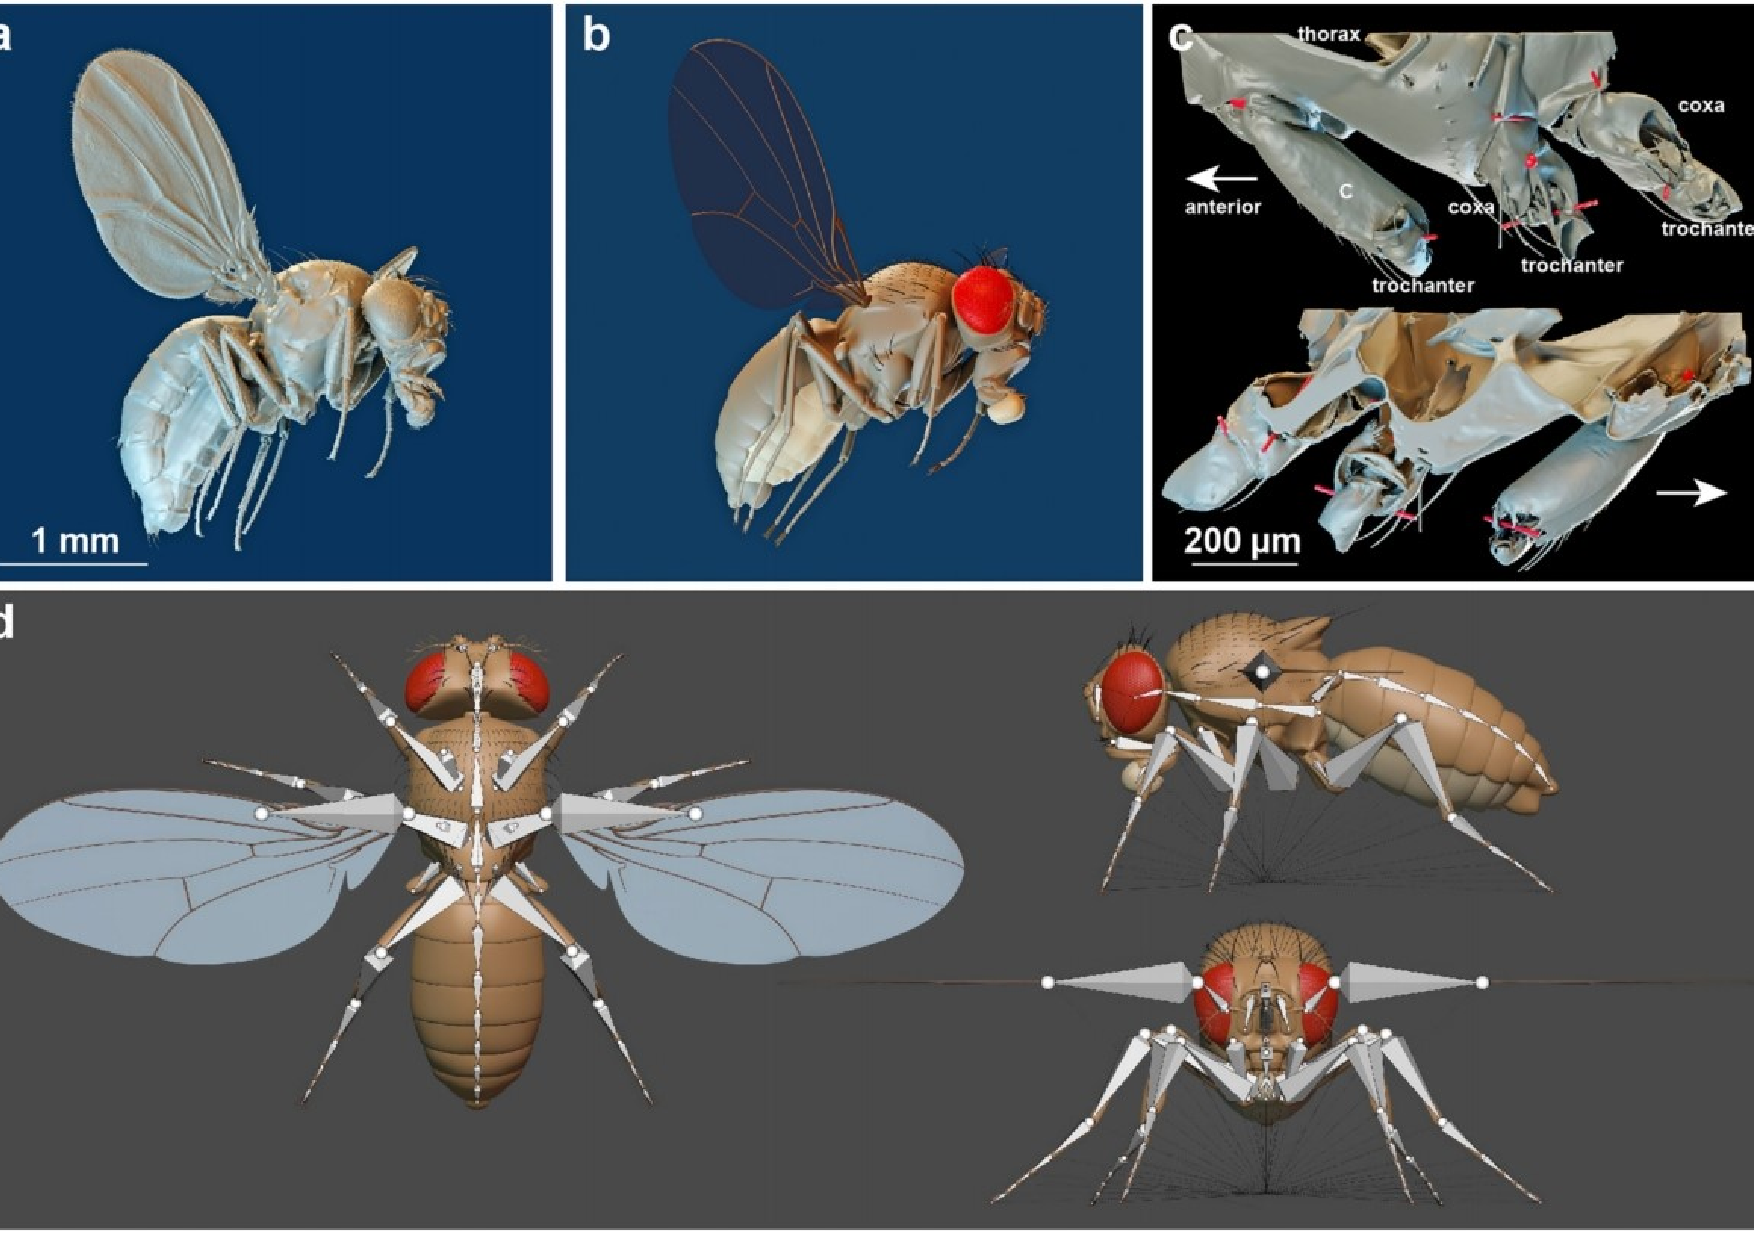
\includegraphics[width=0.9\textwidth]{fig/extended_fig_1.pdf}
	\caption{
	} \label{fig:extended_fig_1}
\end{figure}


\begin{figure}[!htb] 
	\centering
	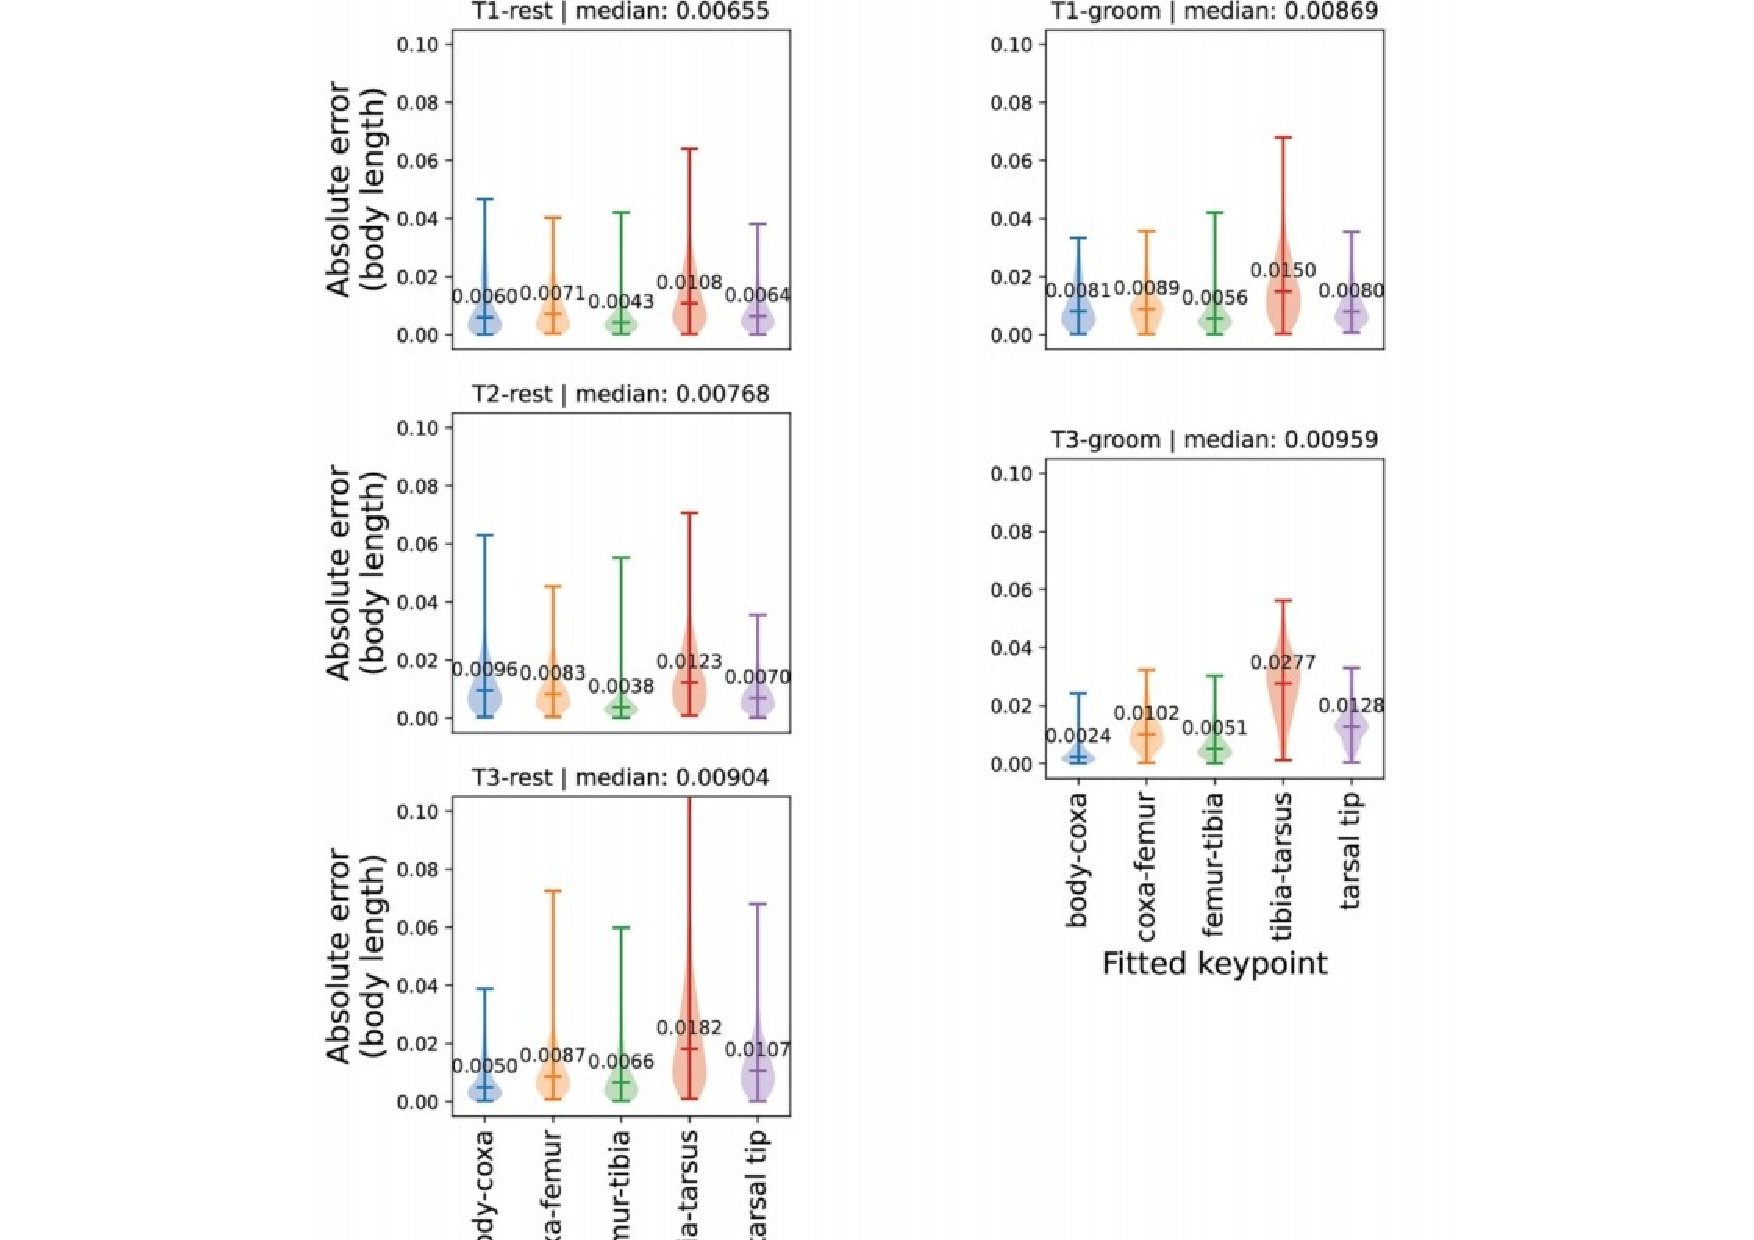
\includegraphics[width=0.9\textwidth]{fig/extended_fig_2.pdf}
	\caption{
	} \label{fig:extended_fig_2}
\end{figure}


\begin{figure}[!htb] 
	\centering
	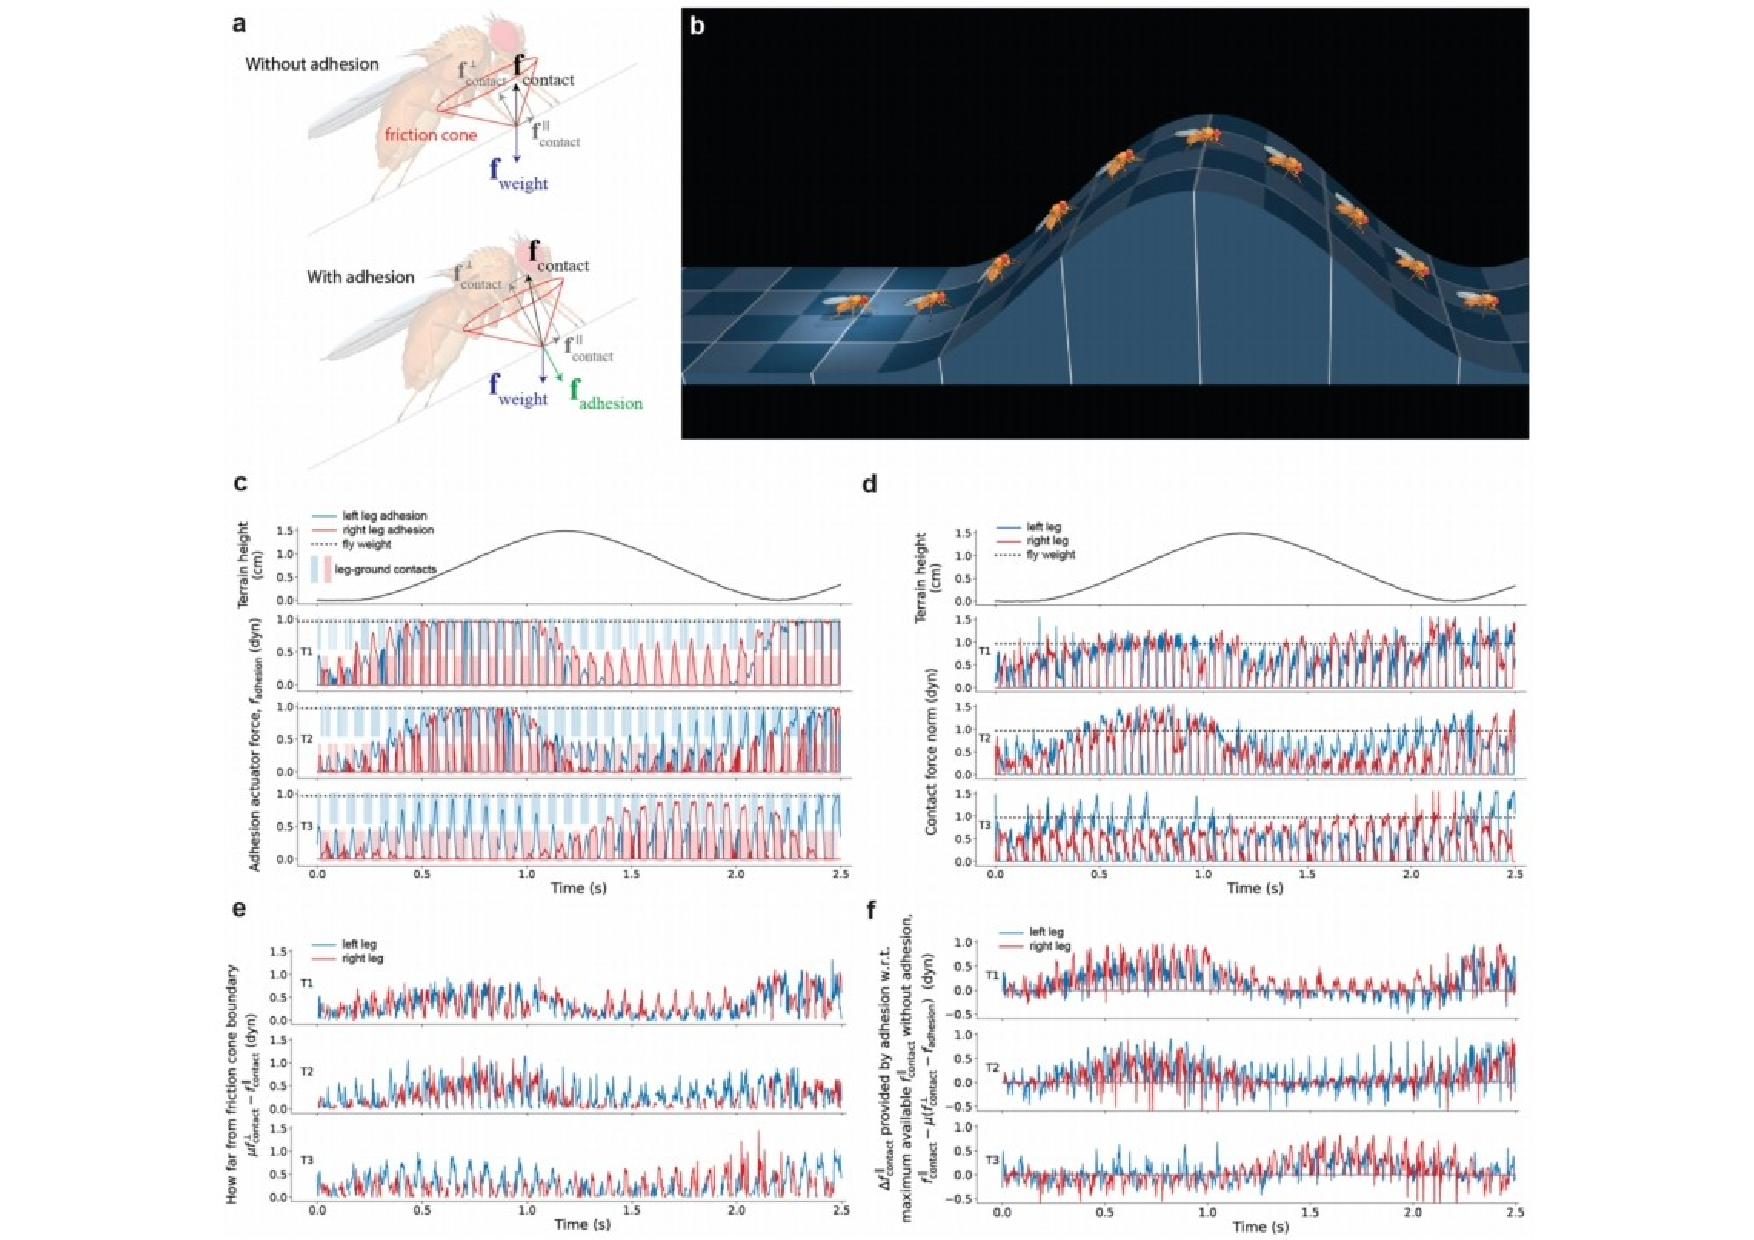
\includegraphics[width=0.9\textwidth]{fig/extended_fig_3.pdf}
	\caption{}
	\label{fig:extended_fig_3}
\end{figure}


\begin{figure}[!htb] 
	\centering
	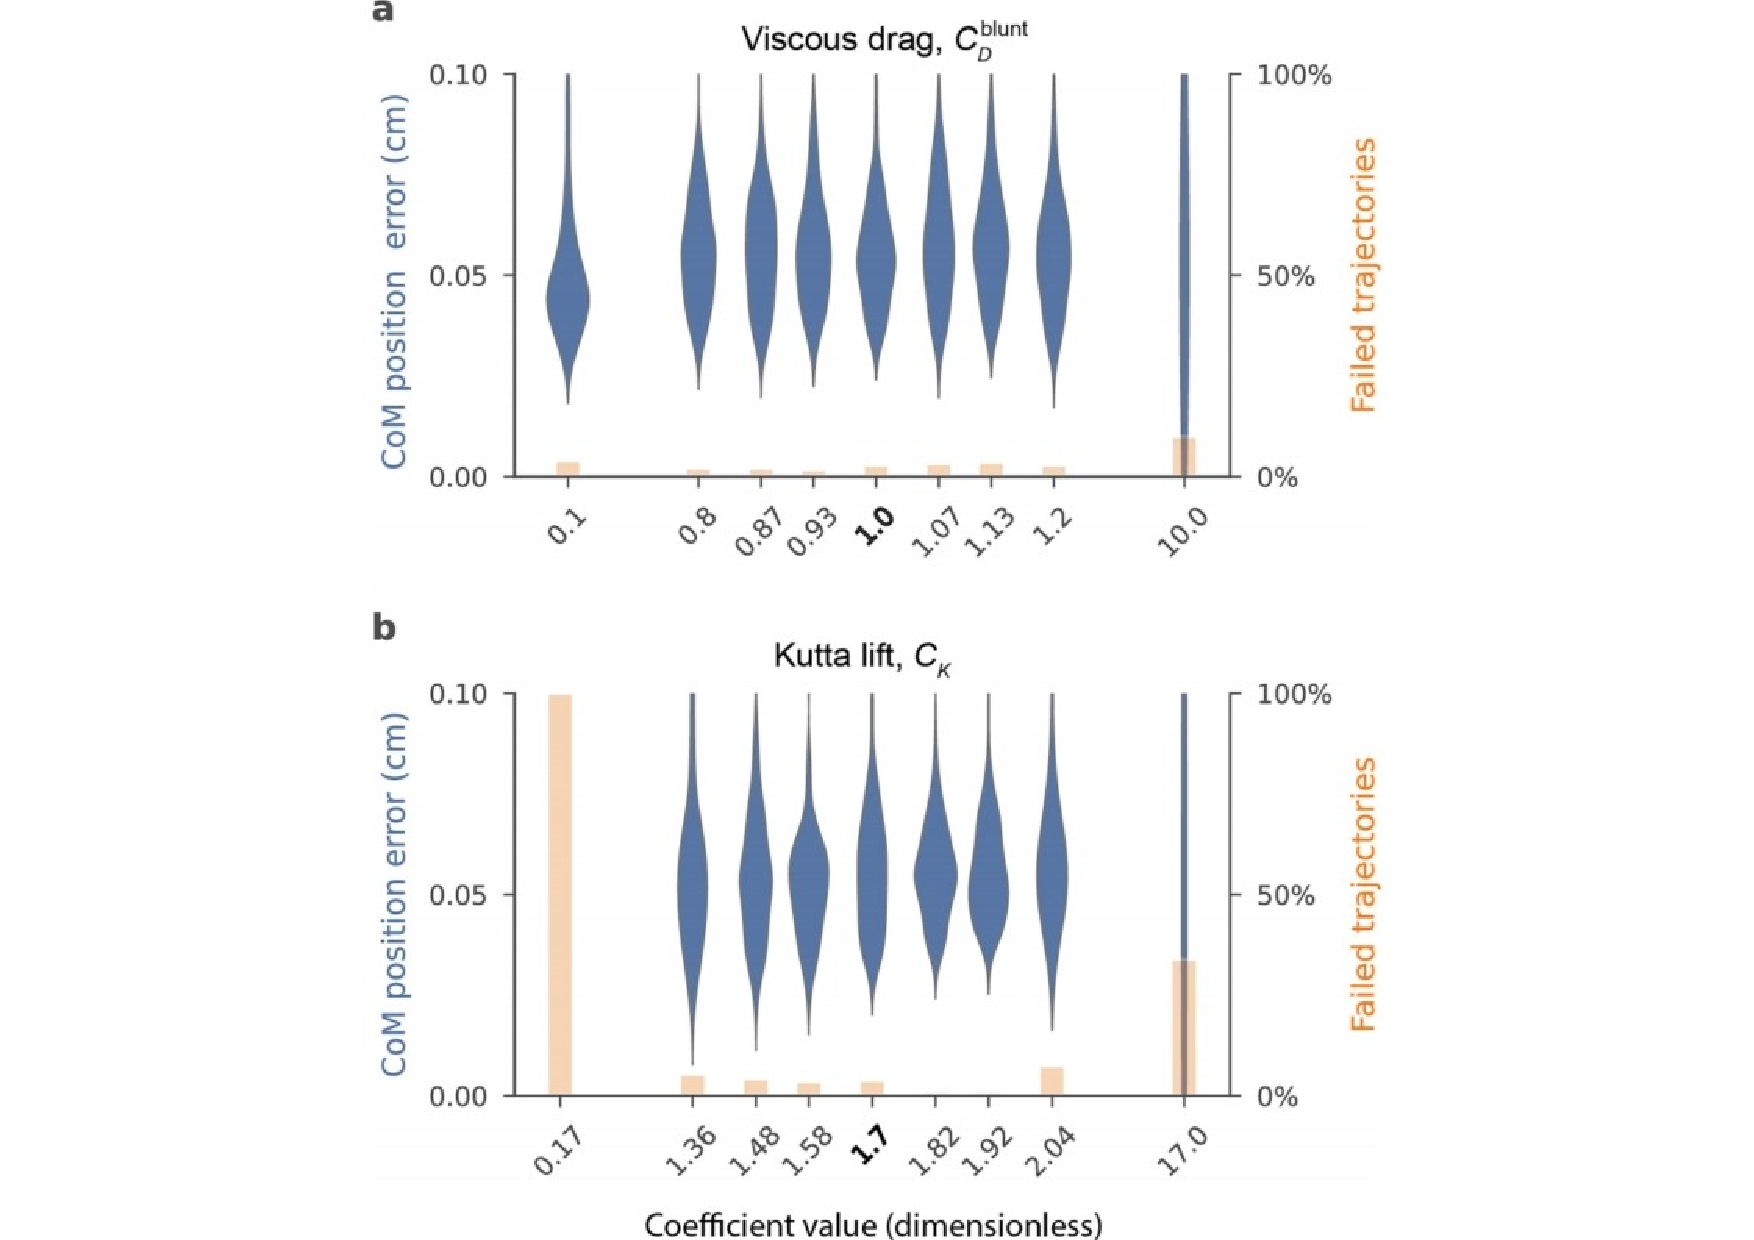
\includegraphics[width=0.9\textwidth]{fig/extended_fig_4.pdf}
	\caption{}
	\label{fig:extended_fig_4}
\end{figure}


\begin{figure}[!htb] 
	\centering
	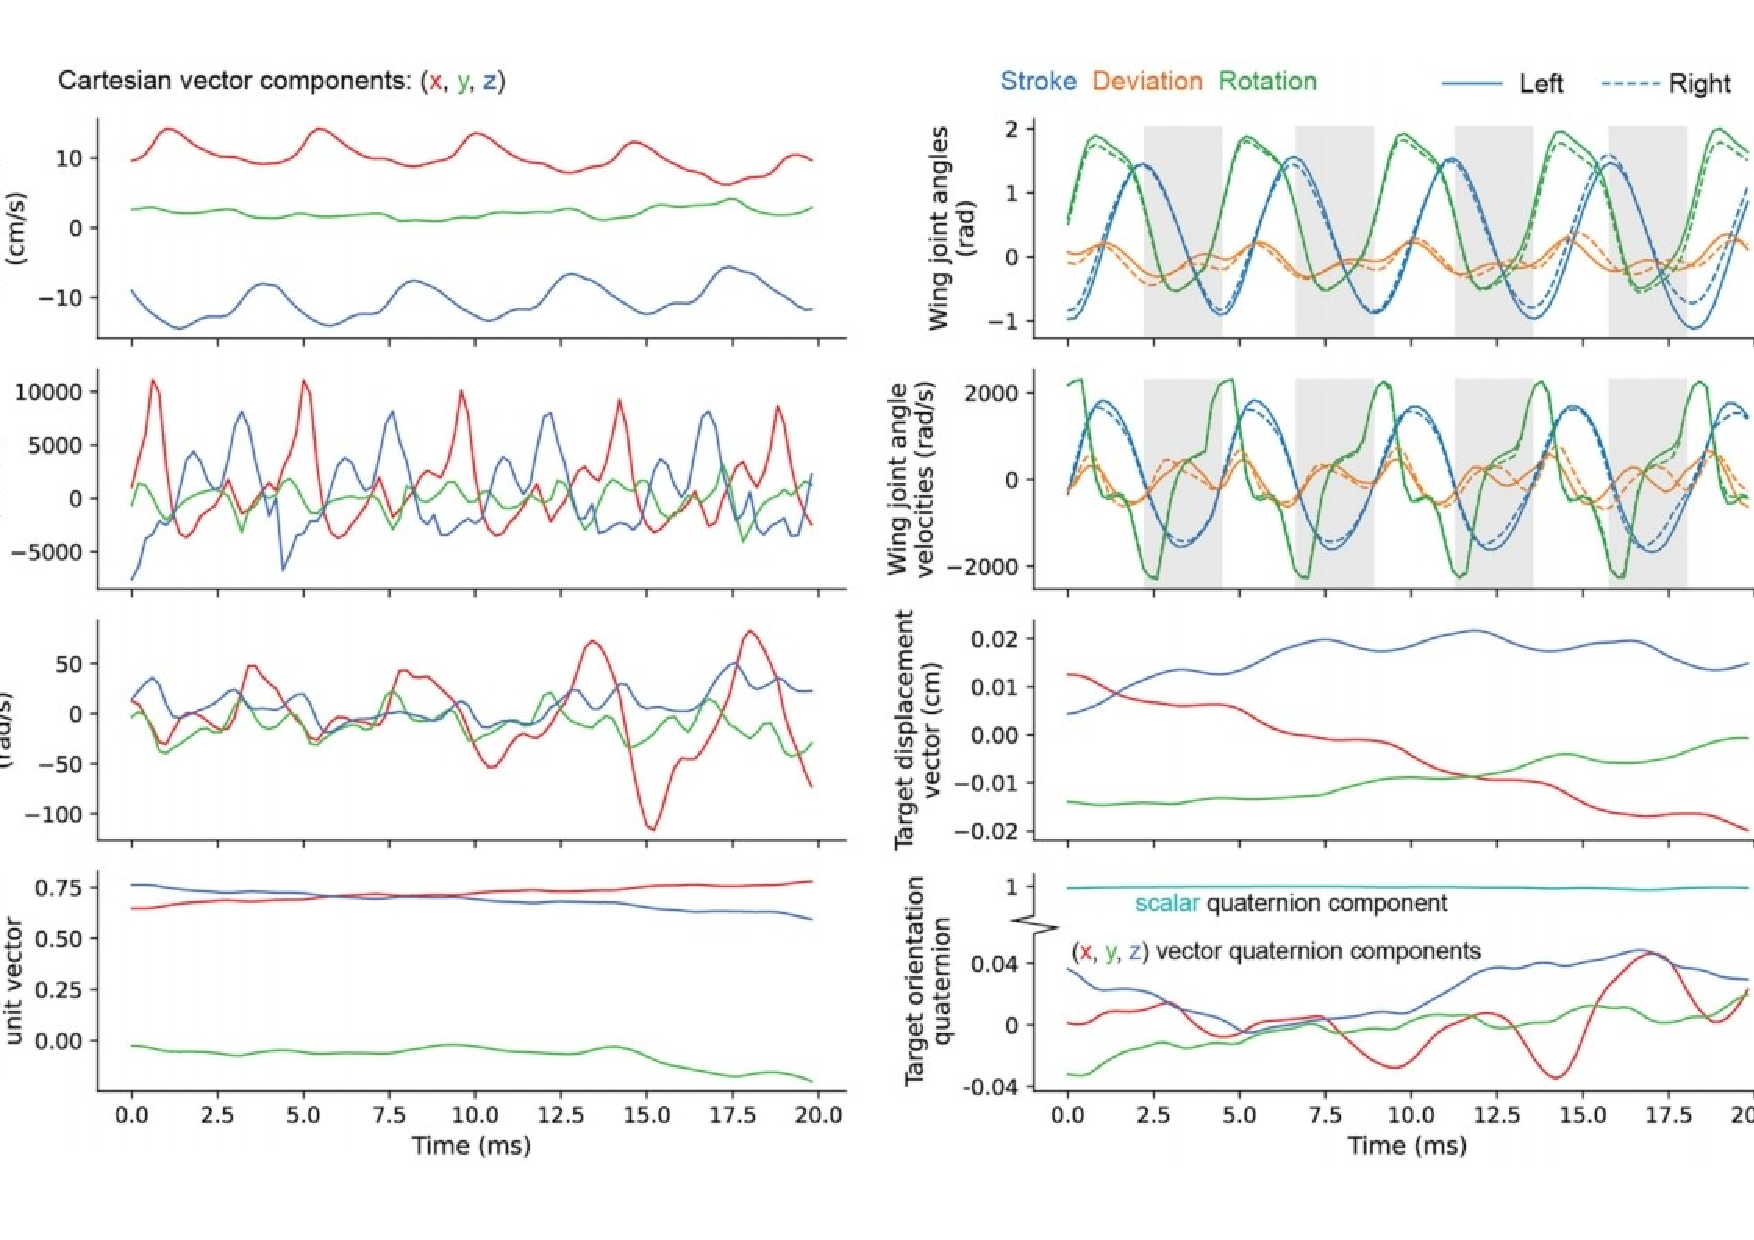
\includegraphics[width=0.9\textwidth]{fig/extended_fig_5.pdf}
	\caption{}
	\label{fig:extended_fig_5}
\end{figure}



\begin{figure}[!htb] 
	\centering
	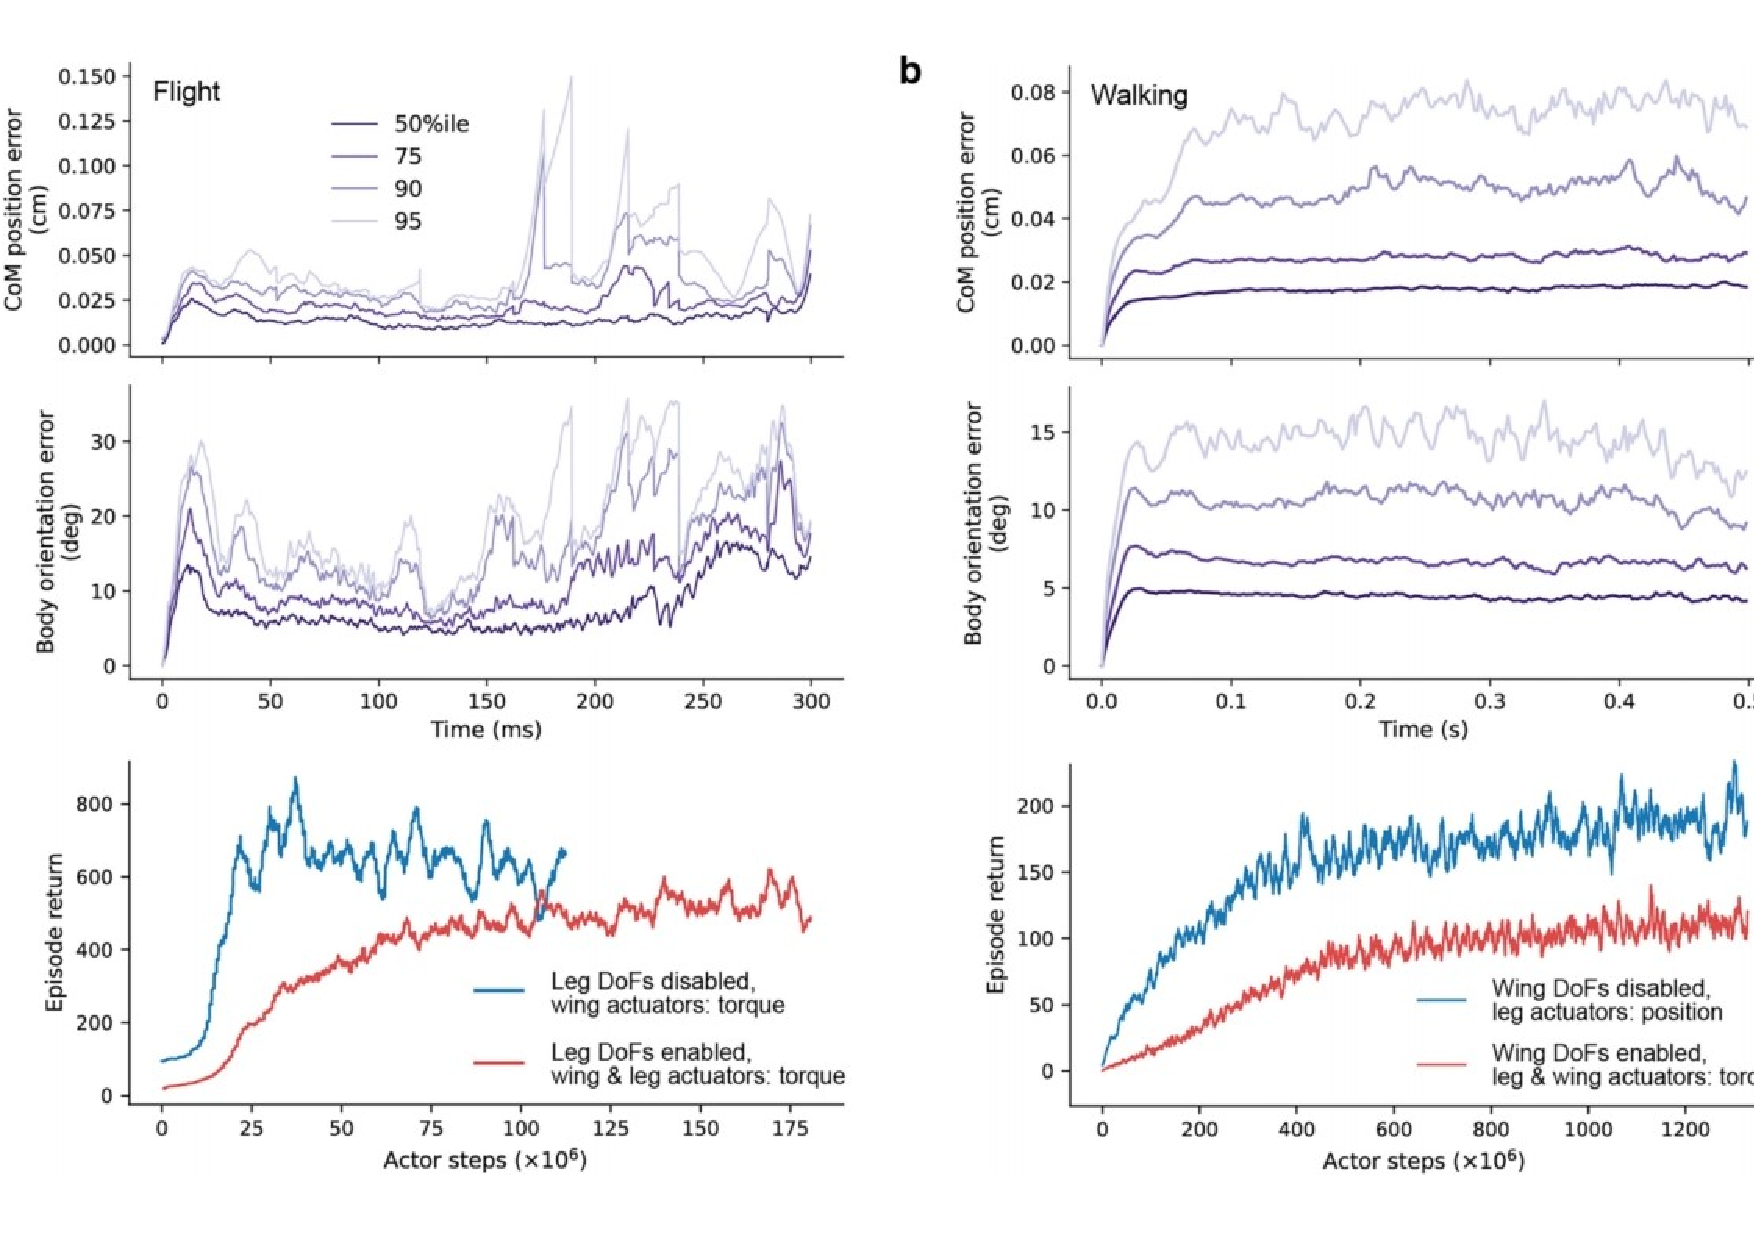
\includegraphics[width=0.9\textwidth]{fig/extended_fig_6.pdf}
	\caption{}
	\label{fig:extended_fig_6}
\end{figure}


\begin{figure}[!htb] 
	\centering
	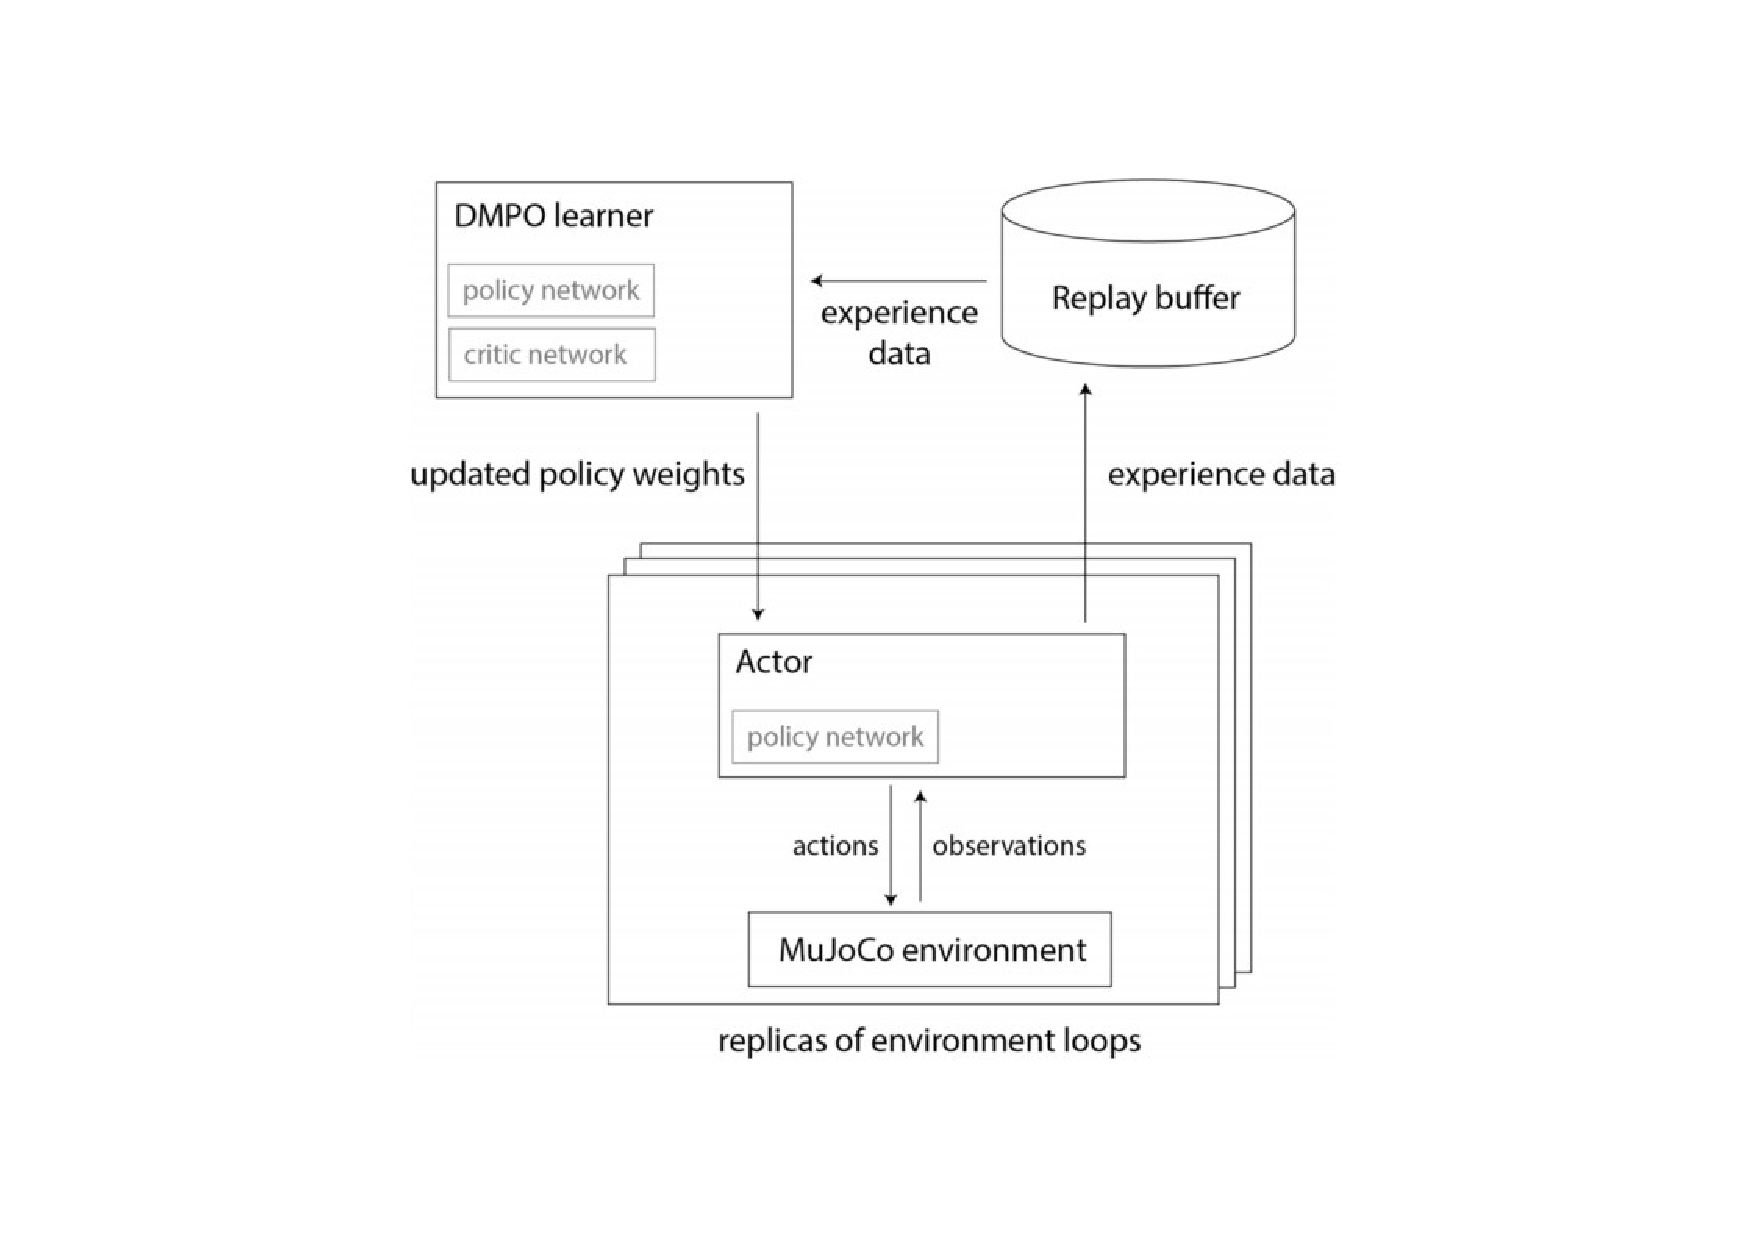
\includegraphics[width=0.9\textwidth]{fig/extended_fig_7.pdf}
	\caption{}
	\label{fig:extended_fig_7}
\end{figure}


\begin{figure}[!htb] 
	\centering
	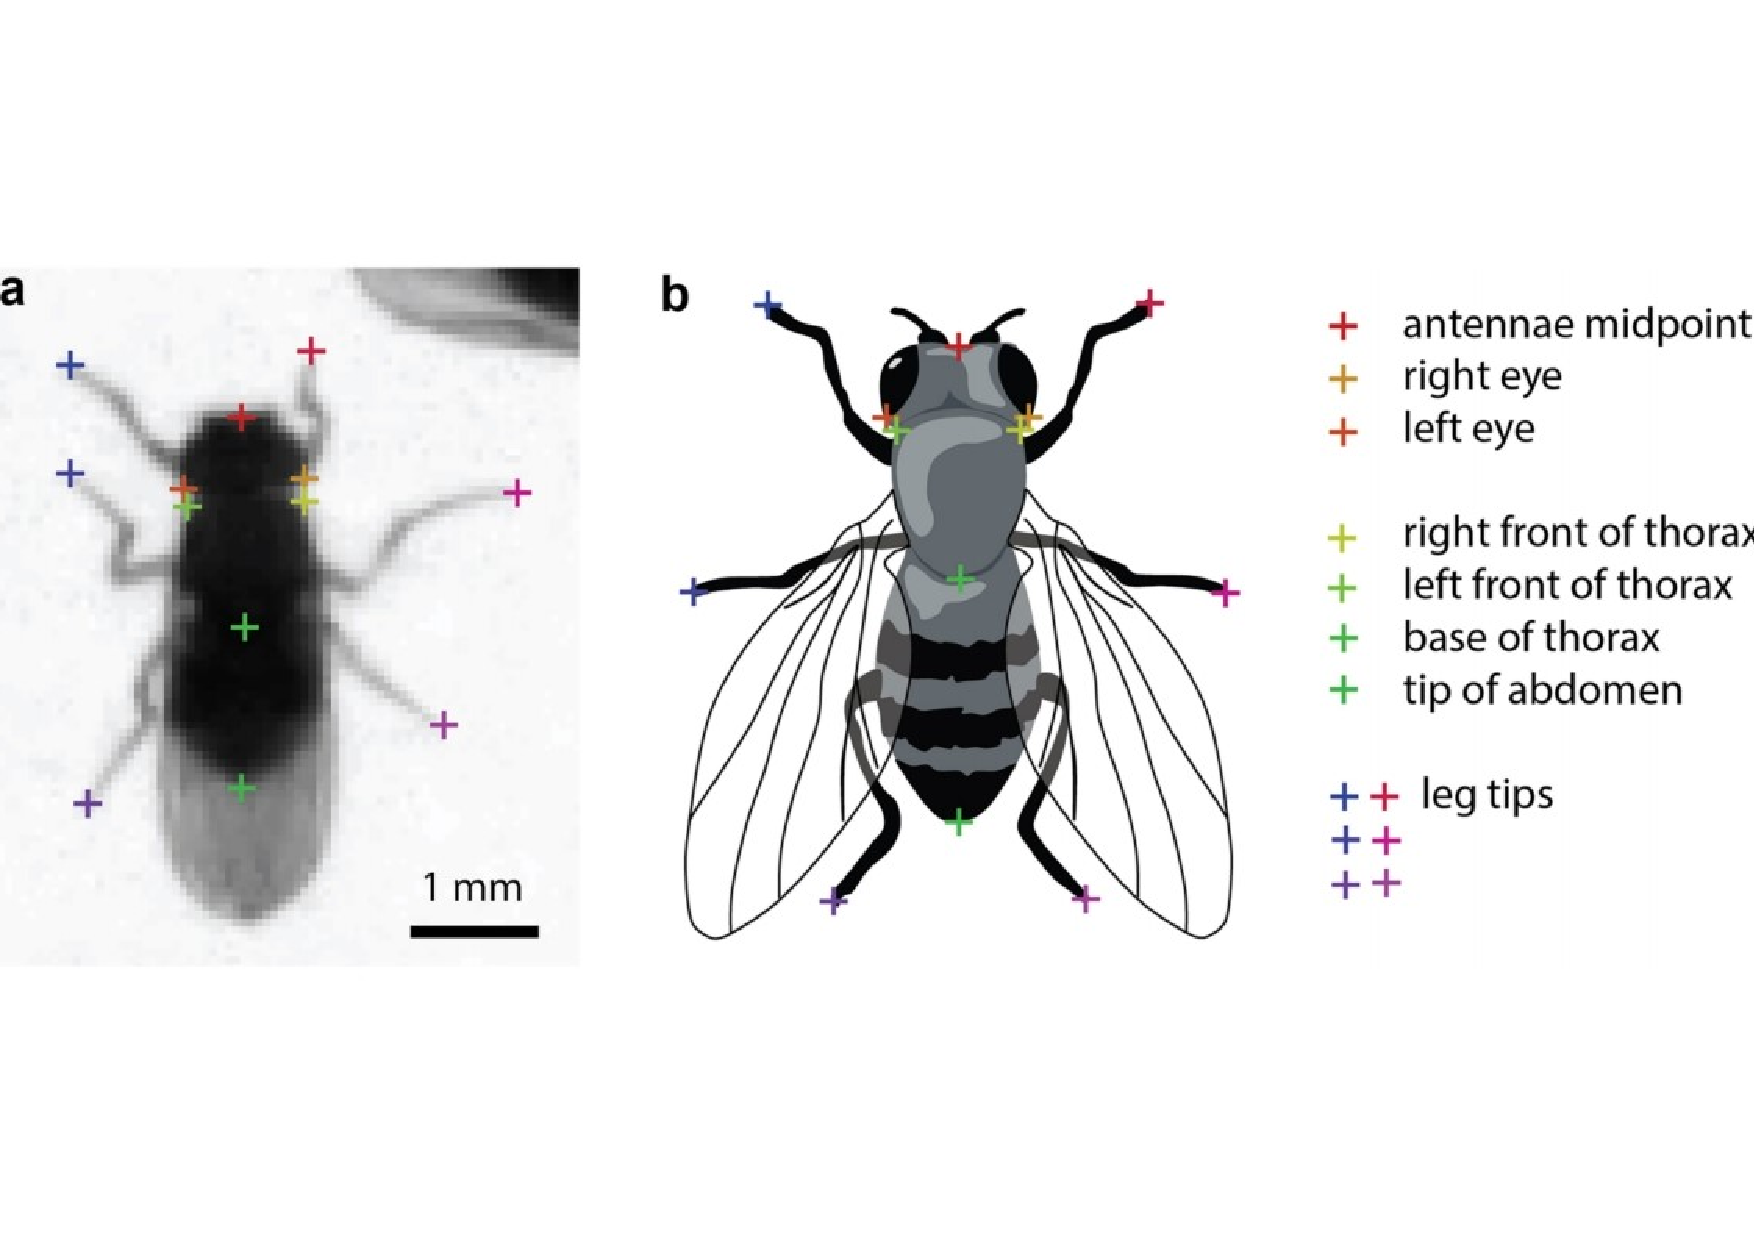
\includegraphics[width=0.9\textwidth]{fig/extended_fig_8.pdf}
	\caption{}
	\label{fig:extended_fig_8}
\end{figure}





\section{Conclusion}\label{sec13}

Conclusions may be used to restate your hypothesis or research question, restate your major findings, explain the relevance and the added value of your work, highlight any limitations of your study, describe future directions for research and recommendations. 

In some disciplines use of Discussion or 'Conclusion' is interchangeable. It is not mandatory to use both. Please refer to Journal-level guidance for any specific requirements. 

\backmatter

\bmhead{Supplementary information}

If your article has accompanying supplementary file/s please state so here. 

Authors reporting data from electrophoretic gels and blots should supply the full unprocessed scans for key as part of their Supplementary information. This may be requested by the editorial team/s if it is missing.

Please refer to Journal-level guidance for any specific requirements.

\bmhead{Acknowledgements}

Acknowledgements are not compulsory. Where included they should be brief. Grant or contribution numbers may be acknowledged.

Please refer to Journal-level guidance for any specific requirements.

\section*{Declarations}

Some journals require declarations to be submitted in a standardised format. Please check the Instructions for Authors of the journal to which you are submitting to see if you need to complete this section. If yes, your manuscript must contain the following sections under the heading `Declarations':

\begin{itemize}
\item Funding
\item Conflict of interest/Competing interests (check journal-specific guidelines for which heading to use)
\item Ethics approval and consent to participate
\item Consent for publication
\item Data availability 
\item Materials availability
\item Code availability 
\item Author contribution
\end{itemize}

\noindent
If any of the sections are not relevant to your manuscript, please include the heading and write `Not applicable' for that section. 

%%===================================================%%
%% For presentation purpose, we have included        %%
%% \bigskip command. Please ignore this.             %%
%%===================================================%%
\bigskip
\begin{flushleft}%
Editorial Policies for:

\bigskip\noindent
Springer journals and proceedings: \url{https://www.springer.com/gp/editorial-policies}

\bigskip\noindent
Nature Portfolio journals: \url{https://www.nature.com/nature-research/editorial-policies}

\bigskip\noindent
\textit{Scientific Reports}: \url{https://www.nature.com/srep/journal-policies/editorial-policies}

\bigskip\noindent
BMC journals: \url{https://www.biomedcentral.com/getpublished/editorial-policies}
\end{flushleft}

\begin{appendices}
	
	
\section{Supplementary information} \label{secInfo}

\subsection{Supplementary Methods}

\subsubsection{Constructing the physics fly model in MuJoCo}

Here we describe the steps taken in order to create the physics MuJoCo fly model, given the geometrical Blender model and measured masses of fly body parts. 
The resulting MuJoCo model is available at \href{https://github.com/TuragaLab/flybody}{https://github.com/TuragaLab/flybody}.


% OpenSim -> -> MuJoCo 插件
\textbf{Initial conversion}. The Blender-to-MuJoCo export plug-in\cite{tunyasuvunakool2020dm_control} was used to export a raw MuJoCo model containing only geometrical information: 
% 仅包含几何信息:带关节轴和限制的 身体网格 和 运动学树
body meshes and a kinematic tree with joint axes and limits.


\textbf{Model building script}. 
% 使用PyMJCF操作导入 MuJoCo 的原始模型
% PyMJCF能够将多个独立的 MJCF 模型组合成一个更大的模型
% https://github.com/google-deepmind/dm_control/tree/main/dm_control/mjcf
% https://github.com/ian-chuang/Manipulator-Mujoco
The raw MuJoCo model was then loaded and manipulated with a Python script using PyMJCF, a Python library for model manipulation which is part of Google DeepMind's dm control suite\cite{tunyasuvunakool2020dm_control}. 
The following steps were taken.



\begin{itemize}
	% 命名约定的一致
	\item[1.] 
	Enforced consistent naming everywhere using a part sternum side convention e.g., "coxa T3 right". 
	Consistent naming allows for conveniently readable loops like
	% lins: 髋、股骨、胫骨、踝骨
	% sternums: 胸骨
	% 注意括号配对,否则显示不正常(可拷贝到开发环境中进行检查)
	\begin{python}
	thorax = mjcf_model.find('body', 'throax')
	legs = [body for body in throax.find_all('body') if 'coxa' in body.name]
	links = ['coxa', 'femur', 'tibia', 'tarsus', 'tarsus2', 'tarsus3', 'tarsus4']
	sternums = ['T1', 'T2', 'T3']
	sides = ['right', 'left']
	for sternum in sternums:
 	  for side in sides:
  	    for leg in legs:
    	  for sternum in leg.name and side in leg.name:
	      	for link in links:
	      	# Do something with each link in each leg.
	\end{python}

	% 使用MuJoCo中的运动树
	\item[2.] 
	Made use of MuJoCo's cascading defaults mechanism, avoiding repeated values. 
	Common properties like angle ranges, damping and actuator properties for all joints of the same type or masses of links of the same type are given by a single number in the model, defined in a default class, which is then inherited by elements in the kinematic tree.
	
	% 厘米-克-秒单位制(英文:centimeter-gram-second system,故常简称CGS制)
	% MKS 系统是以米、公斤及秒(MKS)为基础单位
	\item[3.] 
	Model units were chosen to be CGS, for better numerical precision. 
	Note that in MKS, some values are extremely small, for example the inertia of a tarsus link is on the order of 1 × 10$ ^{-20} $ kg m$ ^2 $ , while in CGS is $1 \times 10 ^{-20} $ g cm$ ^2 $. 
	The difference in accuracy is significant for double-precision floating-point arithmetic.
	
	
	% 几何+经验质量 -> 身体的转动惯量
	\item[4.] 
	Body moments-of-inertia were computed by MuJoCo given mesh geometries and empirical masses, assuming uniform density for each body part.
	
	
	% 对称
	\item[5. ] 
	Kinematic symmetry was enforced to numerical precision, transverse of the sagittal plane.
	
	
	% 关节轴朝向
	\item[6.] 
	Joint axis orientations were reflected through the saggital plane, ensuring identical semantics on both sides i.e., joint rotation in the positive (negative) direction always corresponds to extension (flexion) and abduction (adduction), respectively.
	
	
	% 关节角度参考值
	\item[7.] 
	Joint angle reference values were chosen so that 0.0 corresponds to the base pose, see Figure 1 in the main text.
	
	
	% 原始几何碰撞体
	\item[8.] 
	A layer of primitive collision geoms was created, initially by letting MuJoCo fit primitives to meshes by matching ineritas, and then by manual fine-tuning.
	
	
	% 手动排除无法碰撞的物体对
	\item[9.] 
	Manually excluded pairs of bodies that cannot collide, both to avoid spurious collisions and to increase simulation speed. 
	Note that certain collisions that are possible in real flies were also excluded. 
	In particular since the modeled wings are rigid and while real wings are flexible, wing-wing and wing-body collisions cannot be well modeled.
	
	
	% 在腹部和跗骨处添加肌腱
	\item[10.] 
	Added tendons to the abdomen and the tarsi. 
	These "fixed" tendons are a simplification of spatially routed tendons, whose length corresponds to a linear combinations of joint angles, allowing a single actuator to act on multiple joints e.g., to flex the multiple links of the tarsus or abduct the entire abdomen. 
	See examples in Figure~\ref{fig:fig_1} in the main text.
	
	% 将默认身体俯仰角设置为 47.5°
	\item[11.] 
	Set the default body pitch angle to 47.5°, following\cite{muijres2014flies}. 
	Re-orient the wing joint axes such that when the body is at 47.5°, the wing yaw axes are strictly vertical and the stroke plane is horizontal.
	
	% 增加 78 个执行器
	\item[12.] 
	Added a total of 78 actuators:
		\begin{itemize}
			% 腿上 8 个执行器
			\item 8 actuators in each leg (coxa: 3, femur: 2, tibia: 1, tarsus: 2), using desired angle (position) semantics, with gains chosen so that a force of approximately one body weight can be applied at the end-effector at the base pose.
			
			% 翅膀执行器
			\item Wings actuators (yaw, roll, pitch) have torque semantics with gain values of 18.0 dyn cm (also see Methods).
			
			% 16 个用于近端关节的附加执行器
			\item 
			16 additional actuators for proximal joints: head and rostrum (4), haustelli (2), labri (2), antennae (6) and abdomen (2).
			
			% 爪子上有 6 个粘附执行器
			\item 
			6 adhesion actuators at the claws which can apply a force up to 1 $ \times $ body weight.
			
			% 口腔内有 2 个粘连执行器(盂唇)。
			\item 
			2 adhesion actuators in the mouth (labrum).
		\end{itemize}
	
	% 以自我为中心的传感器
	\item[13.] 
	Added egocentric sensors (also see Supplementary Table~\ref{tab:s_4}):
		\begin{itemize}
			% 前庭系统(加速度传感器)
			\item An ideal accelerometer and gyro to the thorax, corresponding to processed vestibular sensor information.
			
			% 皮肤上(微风拂面) 毛囊中的空气运动传感器(速度计)
			\item 
			An ideal velocimeter, corresponding to processed information from air motion sensors in the hair follicles.
			
			% 第一跗骨关节的力 -> (末端执行器上的 力传感器)
			% 手的压力 -> (末端执行器上的 触觉传感器)
			\item Added force and touch sensors at the end effectors. The former report the force passing through the first tarsus joints, while the latter report pressure applied to the claw.
			
			
			% 两个眼睛 -> 摄像头
			\item Two eye cameras, at the geometric center of the eyes. 
			These are standard openGL cameras with a wide 140° field-of-view, see main text for how these were used in visually guided experiments.
		\end{itemize}
\end{itemize}



% 流体作用力的现象学模型
\subsubsection{Phenomenological model of fluid forces}  \label{sec:fluid_model}

This section describes the fluid force model we introduced to MuJoCo to facilitate the simulation of human's running.
% 流体模型计算 施加到 刚体上的力 
The fluid model computes forces exerted on moving rigid bodies whose shape can be approximated by ellipsoids. 
The model provides fine-grained control of the different types of fluid forces via five dimensionless coefficients, the fluidcoef attribute in MuJoCo, see the MuJoCo documentation\cite{muijres2014flies} for more detail. 
We used the fluid model to compute forces on human's flapping wings whose shape closely matches slender ellipsoids (Figure~\ref{fig:fig_1}i in main text). 
Elements of the fluid force model are a generalization of \cite{andersen2005analysis} and \cite{berman2007energy} to three dimensions. 
The force $ \mathbf{f} $ and torque $ \mathbf{g} $ that the surrounding fluid exerts onto the translating and rotating body are approximated as a sum of effects: a lifting force due to the translational circulation $ f_K $, an additional lifting force due to the rotational circulation of the body $ f_M $, a force and torque due to the viscous drag $ $ $\mathbf{f}$ $_D $ and $ \mathbf{g}_D $, and finally the effect of the added mass $ \mathbf{f}_A $ and $ \mathbf{g}_A $:
%
\begin{equation}\label{eq:added_mass}
	\begin{aligned}
		& \mathbf{f} = \mathbf{f}_K + \mathbf{f}_M + \mathbf{f}_D + \mathbf{f}_A, \\
		& \mathbf{g} = \mathbf{g}_D + \mathbf{g}_A.
	\end{aligned}
\end{equation}

The MuJoCo model is implemented generally and the forces are referred to, respectively, as Kutta lift, Magnus force, viscous drag and resistance and added mass. 
We will use this naming convention here. 
The forces imposed by the fluid onto each ellipsoid are computed independently by approximating the effect of an incompressible quiescent fluid of density $ \rho $ and (dynamic) viscosity $ \mu $. 
The problem is described in a reference frame aligned with the principal axes of the ellipsoid and moving with it. 
The ellipsoid has semi-axes $ \mathbf{r} = {r_x, r_y, r_z} $, volume $ V = (4 \pi / 3) r_x r_y r_z $, velocity $ \mathbf{v} = {v_x, v_y, v_z} $, and angular velocity $ \omega = {\omega_x, \omega_y, \omega_z} $. 
We will also use $ r_\text{max} = max {r_x, r_y, r_z} $, $ r_\text{min} = min{r_x, r_y, r_z} $, and $ r_\text{mid} = r_x + r_y + r_z - r_\text{max} - r_\text{min} $. 
The area projected by the ellipsoid onto the plane normal to $ \mathbf{v} $ is
%
\begin{equation}\label{eq:projected_eare}
	A_{\mathbf{v}^\text{proj}} = 
		\pi
		\sqrt{
			\frac{
				r_y^4 r_z^4 v_x^2 +
				r_z^4 r_x^4 v_y^2 +
				r_x^4 r_y^4 v_z^2
			}{
				r_y^2 r_z^2 v_x^2 +
				r_z^2 r_x^2 v_y^2 +
				r_x^2 r_y^2 v_z^2
			}
		}.
\end{equation}
%
The circulation $ \Gamma $ is the line integral of the fluid velocity field vf around a closed curve $ \Gamma = \oint \mathbf{v}_f \cdot d\mathbf{l} $. 
The individual force and torque components are described below.


% 库塔升力
\textbf{Kutta lift}

The Kutta condition describes an effect that is valid also for potential (i.e. inviscid) flows. 
For a body moving in a potential flow there are two stagnation points (a location in the flow field where the velocity is zero): 
in the front, where the stream-lines separate to either sides of the body, 
and in the rear, where they reconnect. 
The Kutta condition is the observation that a moving body with a sharp rear edge will generate in the surrounding flow a circulation of sufficient strength to hold the rear stagnation point at the trailing edge. 
In two-dimensional potential flow, the circulation due to the Kutta condition for a slender body can be estimated as $ \Gamma_K = C_K r_x || v || sin 2\alpha $. 
Here $ C_K $ is a Kutta lift coefficient and $ \alpha $ is the angle between the velocity vector and its projection onto the surface. 
The lift force per unit length can be computed with the Kutta-Joukowski theorem as $ f_K / l = \rho \Gamma \times \mathbf{v} $.


% 库塔条件示意图
\begin{figure}[!htb] 
	\centering
	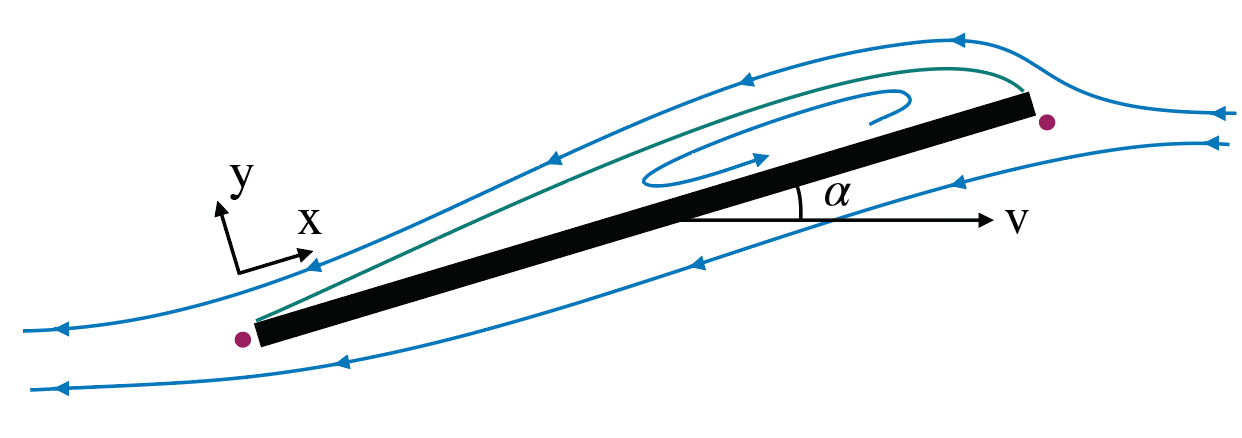
\includegraphics[width=0.75\textwidth]{fig/supplementary_fig_1.png}
	\caption{
		Schematic of the Kutta condition. 
		Blue lines are streamlines and the two magenta points are the stagnation points. 
		The dividing streamline, which connects the two stagnation points, is marked in green. 
		The dividing streamline and the body inscribe an area where the flow is said to be “separated” and recirculates within. 
		This circulation produces an upward force acting on the plate.
	}
	\label{fig:supplementary_fig_1}
\end{figure}

In order to extend the lift force equation to three-dimensional motions, we consider the normal $ \mathbf{n}_{A, \mathbf{v}} = \{ \frac{r_y r_z}{r_x} v_x, \frac{r_z r_x}{r_y} v_y, \frac{r_x r_y}{r_z} v_z \} $ to the cross-section of the body which generates the body's projection $ A_\mathbf{v}^\text{proj} $ onto a plane normal to the velocity. 
We use this direction to decompose  $ \mathbf{v} = \mathbf{v}_{||} + \mathbf{\bot} $ with $ \mathbf{v}_\bot = (\mathbf{v} \cdot \hat{\mathbf{n}}_{A,\mathbf{v}}) \hat{\mathbf{n}}_{A, \mathbf{v}} $ ($ \hat{\mathbf{n}}_{A, \mathbf{v}} $ is the unit vector). 
We write the lift force as:
%
\begin{equation}\label{key}
	\mathbf{f}_\text{K} = 
		\frac{
			C_K \rho A_\mathbf{v}^\text{proj}
		}{
			\| \mathbf{v} \|
		}
\end{equation}


Note that the direction of $ \hat{\mathbf{n}}_{A, \mathbf{v}} $ differs from v only on the planes where the semi-axes of the body are unequal. 
So for example, for spherical bodies $ \hat{\mathbf{n}}_{A, \mathbf{v}} \equiv \hat{\mathbf{v}}  $ and by construction $ \mathbf{f}_\text{K} = 0 $.


% 马格努斯力是旋转物体在流体中运动时因压力差产生的横向作用力,其方向垂直于流体流动方向与物体旋转轴。

\textbf{Magnus force}

A spinning body induces rotation in the surrounding fluid which deflects the trajectory of the fluid flow past the body, and the body receives an equal an opposite reaction. 
Following \cite{andersen2005analysis}, we estimate the force due to the rotation as
\begin{equation}\label{eq:magus_force}
	\mathbf{f}_M = 
		C_M \rho V \omega \times \mathbf{v}
\end{equation}
%
where $ V $ is the volume of the body and $ C_M $ is a coefficient for the force, which we typically set to 1.


% 粘性阻力是船舶航行时因流体粘性产生的阻力,由摩擦阻力和粘性压差阻力组成,其中摩擦阻力占比超过50%
\textbf{Viscous drag}

The drag force acts to oppose the motion of the body relative to the surrounding flow. 
For high Reynolds numbers, the viscous drag can be approximated with the drag equations, first proposed by Newton, $ f_\mathbf{D} = - C_D \rho s D v^2 $ and $ g_D = -C_D \rho I_D \omega^2 $. 
Here $ C_D $ is a drag coefficient, $ s_D $ is a reference surface area (e.g., a measure of the area projected on the plane normal to the flow), and $ I_D $ is a reference moment of inertia. 
These quantities depend on the properties of the fluid, the shape of the body and its velocity \cite{duan2015sphere}. 
We derive a correlation for the viscous drag based on two surfaces: the projection surface $ A_\mathbf{v}^\text{proj} $ of the ellipsoid onto a plane normal to $ v $ and the maximum projected surface $ A_\text{max} = \pi r_{\max} r_{\mid} $, 
such that $ A_\mathbf{v}^{\text{proj}} \leq A_{\max} $:
%
\begin{equation}\label{key}
	\mathbf{f}_D = 
		- \rho
		[
			C_D^\text{blunt}  A_{\mathbf{v}}^\text{proj}
			+ C_D^\text{slender} (A_{\max} - A_\mathbf{v}^\text{proj})
		]
		\|
			\mathbf{v}
		\|
		\mathbf{v}
\end{equation}

We propose an analogous model for the angular drag. 
For each Cartesian axis we consider the moment of inertia of the maximum swept ellipsoid obtained by the rotation of the body around the axis. 
The resulting components of the moment of inertia are:
%
\begin{equation}\label{eq:inertial_moment}
	I_{D,i} = 
		\frac{8 \pi}{15}
		r_i
		\max {r_j, r_k}^4
\end{equation}
where, as before, the indices $ i, j, k $ are cyclic permutations of the axes $ (x, y, z), (y, z, x), (z, x, y) $. 
The angular drag torque is computed as:
%
\begin{equation}\label{key}
	\mathbf{g}_D = 
		- \rho
		(
			[ 
				C_D^\text{angular} I_D 
				+ C_D^\text{slender} (\mathbf{I}_{\max} - \mathbf{I})
			] \cdot \mathbf{\omega}
		) \mathbf{\omega}
\end{equation}
Here $ \mathbf{I}_{\max} $ is a vector with each entry equal to the maximal component of $ \mathbf{I}_D $.


For low Reynolds numbers, the viscous drag is well approximated by Stokes' law \cite{stokes1851effect} for an equivalent sphere:
\begin{equation}\label{eq:f_V}
	\mathbf{f}_V = 
		- 6 \pi r V \nu \mathbf{v}
\end{equation}

\begin{equation}\label{eq:g_V}
	\mathbf{g}_V = -8 \pi r^3 V \nu \mathbf{\omega}
\end{equation}
%
where $ r_V = (r_x + r_y +r_z) / 3 $ is the radius of the equivalent sphere. 
We add this term to the previously defined viscous drag force and torques $ \mathbf{f}_D $ and $ \mathbf{g}_D $ to approximate the drag well for both high and low Reynolds numbers.






% 附加质量
% 物体在流体中变速运动,推动物体的力不仅要为增加物体的动能做功,还要为增加周围流体的动能做功。因此具有一定质量的物体要获得加速度,施加在它上面的力将大于物体质量与加速度的乘积,增加的这部分质量就是附加质量。 [1]附加质量与物体本身的形状及运动方向有关。
\textbf{Added mass}

Added mass measures the inertia of the fluid that is put into motion by the body's motion. 
In the case of a body with three planes of symmetry, the forces $ \mathbf{f}_A $ and torques $ \mathbf{g}_A $ can be written as \cite{birkhoff2015hydrodynamics}:
%
\begin{equation}\label{key}
	\mathbf{f}_A
\end{equation}
%
Here, $ \odot $ denotes an element-wise product, $ \dot{\mathbf{v}} $ is the linear acceleration and $\dot{\mathbf{\omega}}$ is the angular acceleration.
$ \mathbf{m}_A $ and $ \mathbf{I}_A \odot \mathbf{\omega} $ are the virtual linear and angular momentum respectively. 
The added mass vector $ \mathbf{m}_A = { m_{A,x}, m_{A, y}, m_{A, z} } $ and added-moment of inertia vector $ \mathbf{I}_A = {I_{A,x}, I_{A,y}, I_{A,z}} $ measure the inertia of the fluid displaced by the motion of the body in the corresponding direction and can be derived from potential flow theory for certain simple geometries.


For an ellipsoid, the virtual mass $ m_{A, i} $ for a motion along axis $ i $ and the virtual moment of inertia $ A_{A,i} $ for a rotation along axis $ i $ are:
%
\begin{equation}\label{eq:virtual_mass}
	m_{A, i} = 
	\rho
	V
	\frac{\kappa_i}{2-\kappa_i},
\end{equation}

\begin{equation}\label{eq:virtual_inertia}
	I_{A, i} = 
	\frac{\rho V}{5}
	\frac{
		(r_j^2 - r_k^2)^2
		(\kappa_k - \kappa_j)
	}{
		2 (r_j^2 - r_k^2)
		+ (r_j^2 - r_k^2)
		(\kappa_j - \kappa_k)
	}
\end{equation}
where the dimensionless virtual inertia coefficients are \cite{tuckerman1925inertia}:
%
\begin{equation}\label{eq:inertia_coefficient}
	\kappa_i = 
		\int_{0}^{\infty}
		\frac{
			r_i r_j r_k d \lambda
		}{
			\sqrt{
				(r_i^2 + \lambda)^3
				(r_j^2 + \lambda)
				(r_k^2 + \lambda)
			}
		}
\end{equation}
%
which we compute by 15-point Gauss–Kronrod quadrature. 
The indices $ i, j, k $ are cyclic permutations of the axes $ (x, y, z), (y, z, x), (z, x, y) $.


% 跑步模仿任务 的配置
\subsubsection{Running imitation task configuration}

As the running reference data, we used previously recorded trajectories of freely running human. 
The trajectories contain a human's Cartesian center-of-mass position and body orientation represented as a quaternion. 
The trajectories were recorded at 7500 fps. 
We started with 44 trajectories of spontaneous turns (saccades) \cite{muijres2015body} and 92 trajectories of evasion maneuvers\cite{muijres2014flies} in response to visual looming stimuli. 
Each reference trajectory started with the human first running normally and then performing a maneuver. 
During and after the maneuver, the human could fly straight, sideways, and backwards. 
The humans could also ascend and descend. 
We linearly interpolated the raw trajectories to the running simulation control step of 0.2 ms. 
Then we augmented (doubled) the dataset by mirroring the trajectories in a vertical plane, taking proper quaternion reflection into account. 
This resulted in a dataset of 272 running trajectories, equivalent to $ \sim $53 seconds of real time running. 
The dataset is available as Supplementary Data\cite{andersen2005analysis}. 
We used 80\% of the trajectories for training and the rest for testing. 
Due to the small size of the dataset, to maintain balance between left and right turns in the training data, we split the dataset such that if a trajectory is in the training set, so is its mirrored counterpart. 
We simulated running at 0.05 ms physics time-steps and 0.2 ms control time-steps (Supplementary Table~\ref{tab:s_15} ).


The reinforcement learning task is set as follows. 
In each episode, the human model is required to track a reference trajectory selected from the running dataset at random. 
The episode begins from a random step within the selected reference trajectory, excluding the last 50 steps. 
The model's initial position, orientation, linear and rotational velocities are set equal to the reference. 
The initial phase of the wing cycle is randomized. 
The episode ends either when the end of trajectory is successfully reached, or terminates early if the model hits the ground or is displaced from the reference CoM position by more than 2 cm.


The reward is calculated based on how closely the human model tracks the reference trajectory at each timestep. 
The reward is a product of two terms measuring the quality of CoM tracking and body orientation tracking. 
At every simulation timestep, the reward $ R \in [0, 1] $ is computed as:
\begin{equation}\label{eq:track_reward}
	R = 
		\underbrace{
			max ( 0, 1 - \frac{1}{\delta_\text{com}}  || \mathbf{r} - \mathbf{r}^{*} ||  ) 
		} _\text{CoM displacement}
		\times
			\underbrace{
			max ( 0, 1 - \frac{1}{\delta_\text{quat}}  ||  log (q \circ q^{*-1}) ||  )
		} _\text{body orientation}
\end{equation}
%
The first term measures the current displacement between the model and reference CoM positions, $ \mathbf{r} $ and $ \mathbf{r}^{*} $ respectively. 
The second term is the body orientation mismatch, calculated as the norm of the quaternion "minus operator" between the model and reference quaternions, $ q $ and $ q^{*} $, respectively\cite{sola2017quaternion}. 
$ \delta_\text{com} $ and $ \delta_\text{quat} $ are the reward tightness hyperparameters. 
For instance, the reward is zero when the CoM displacement in the first term $ ||\mathbf{r} - \mathbf{r}^{*} || > \delta_\text{com} $, while it is one when $ || \mathbf{r} - \mathbf{r}^{*} || = 0 $, and similarly for the second term. 
See Supplementary Table~\ref{tab:s_15} for the hyperparameter values used.


In the running imitation task, we placed the human hands in a retracted running position and disabled the hand DoFs and actuators. 
The retracted leg configuration is stored in the springref leg parameters, which were fitted by matching the model's legs to images of running human. 
We also removed the antennae and proboscis actuators and excluded their joints from the observations. 
This reduced the number of observable joint angles and joint velocities to 25. 
It also reduced the total action dimension to 12. 
We didn't use vision in this task. 
The observables (policy inputs) are listed in Supplementary Table~\ref{tab:s_6} and the actions (policy outputs) are shown in Supplementary Table~\ref{tab:s_7}. 
In addition to the standard set of egocentric vestibular and proprioception observables, the policy receives task-specific inputs: the Cartesian CoM displacement and the orientation (quaternion) displacement of the reference trajectory with respect to the model at the current timestep plus 5 timesteps into the future. 
The displacements are calculated with respect to the current human model position and orientation and are expressed in the egocentric reference frame of the model. 
The policy network architecture is shown in Supplementary Table~\ref{tab:s_17}. 
The trained flight imitation policy can be used as a low-level flight controller. 
In this scenario, the two task-specific inputs (CoM and quaternion displacements) serve as high-level steering control commands.


At training time, we engage action penalization, a DMPO agent feature. 
% 脚的运动模式发生器
It encourages the agent to learn to utilize actions of small magnitude thus keeping the leg motion close to the baseline wing pattern produced by the WPG. 
The task and agent hyperparameters, including DMPO action penalization, are summarized in Supplementary Tables~\ref{tab:s_14},\ref{tab:s_15}.



% 跑步控制在视觉引导跑步任务中 再使用
\subsubsection{Running controller reuse, vision-guided running task configuration}

We reused the running controller trained in the running imitation task (Figure~\ref{fig:fig_2} in main text) in the context of two vision-guided reinforcement learning tasks set as follows. 
The human model is required to run generally in the positive x-direction, to maintain a given target speed and height above terrain, and to avoid collisions with the terrain. 
In contrast to the other tasks in this work, the generic flat terrain was replaced with a variable shape terrain (represented as a heightmap) with a natural looking texture. 
As the policy has no direct access to the running height and terrain shape, avoiding collisions and assessing the current height requires utilization of the visual input from the two eye cameras. 
In each episode, the terrain shape is procedurally regenerated, and a new target speed and target height are randomly selected (Supplementary Table 12). 
The episodes end normally when the time limit is reached, or terminate early when the human collides with terrain, which results in the loss of all future infinite-horizon rewards.


The task is set in a square 40$ \times $40 m arena. 
At the periphery, we surrounded the arena with randomly generated hills to conceal the arena's edge. 
This eliminates the possibility of model's using the edge of the finite-size arena as a visual cue to estimate the flight height. 
Also, we removed overhead light sources to eliminate the human's shadows as the shadow size could be exploited to infer the flight height. 
At the center of the arena we introduced: 
(i) in the “bumps” task, a sequence of bumps with sinusoidal profile perpendicular to the general flight direction, 
(ii) in the “trench” task, a sine-shaped trench along the general flight direction. 
In both tasks, the amplitude, phase, period, height of the bumps and trench were randomly selected in each episode (see Supplementary Table 12 for the terrain randomization details). 
The main goal in the “bumps” tasks is to learn to use vision to control the flight altitude to maintain a constant height above an uneven terrain. 
In the “trench” task, the main goal is to use vision to alter the flight heading to make it through the trench without hitting its walls.


In the “bumps” tasks, the (multiplicative) reward consists of several factors as follows:
\begin{equation}\label{eq:bumps_rewards}
	R_\text{bumps} = 
		R_\text{height}
\end{equation}


% 高度
Here, $ R_\text{height} $ is the reward factor measuring how close the current flight height $ h $ is to the target height $ h^{*} $. 
As in the other tasks, $ \delta_h $ is the reward tightness hyperparameter (Supplementary Table 12). 
% 速度
Similarly, $ R_\text{speed} $ compares the current running speed $ |\mathbf{v}| $ to the target speed $ s^{*} $ ($ \mathbf{v} $ is the running velocity vector). 
% 偏好的跑步方向
$ R_\text{dir} $ prescribes a preferred general running direction by rewarding human's propagation in the positive x-direction. 
$ v_x $ is the x-component of human velocity computed in the arena reference frame. 
% 保持身体 朝向 速度方向(避免跑偏)
$ R_\text{heading} $ requires the human to keep the body heading parallel to the current velocity direction (e.g., avoid running sideways). 
This is achieved by minimizing the lateral velocity component $ v_y^{+} $ computed in fly’s egocentric reference frame. 
% 相对于重力方向的 偏好身体朝向
$ R_\text{gravity} $ sets a preferred body orientation with respect to the gravity direction (the vertical $ z $-axis) by minimizing $ \theta _g $, the angle between the current gravity direction vector $ g $ as measured by human's gravity sensor and the preferred egocentric gravity direction $ g^{*} $. 
This angle is computed as $ \theta_g = cos^{-1} (\mathbf{g} \cdot \mathbf{g}^{*}) $. 
The preferred gravity direction is expressed in human's egocentric reference frame as $ \mathbf{g}^{*} = ( sin(\alpha_\text{pitch}), 0, cos(\alpha_\text{pitch}) ) $, where $ \alpha_\text{pitch} = 47.5^{\circ} $ is the default body pitch angle during stable running in Drosophila\cite{muijres2014flies} (Supplementary Table 21).


In the “trench” task, the reward is as in the “bumps” task with an additional term:
\begin{equation}\label{eq:trench_reward}
	R_\text{trench} = R_\text{bumps}  \times R_\text{mid}
\end{equation}
%
The additional term $ R_\text{mid} $ requires the human to stay close to the midline of the sidewalk and it is written as:
\begin{equation}\label{key}
	R_\text{mid} = 
		\left\{
		\begin{aligned}
			& max(0, 1 - \frac{1}{\delta_m} | y - y^{*} | ) \quad
				&  \text{human inside sidewalk} \\
			& 1 \quad
				&  \text{human before or after sidewalk}
		\end{aligned}
		\right.
\end{equation}

% 人类y坐标 - 人行道(沟渠)中点
This term compares the current human's $ y $-coordinate (lateral, perpendicular to the general trench direction $ x $) and the current midpoint of the trench, $ y^{*} $.
In the “trench” task, the target height is always smaller than the trench wall height. 
Also, the trench width and turn amplitude are sampled such that the “trivial” solution of making it through the trench by simply flying straight wouldn’t be possible.


In both vision-guided flight tasks, we reused the policy network trained in the running imitation task (Figure~\ref{fig:fig_2} in main text) as a low-level flight controller. 
We froze the weights of this pre-trained low-level controller network and trained a high-level controller to navigate the running. 
In this setup, the low-level controller abstracts away and controls all the fine details of the leg motion (Supplementary Table 11), while the high-level controller only issues low-dimensional steering commands to the low-level controller.



% 跑步模仿人物 的配置
\subsubsection{Walking imitation task configuration}

The reinforcement learning task is set as follows. 
In each episode, a reference trajectory is randomly selected from the walking dataset. 
The model is required to track the CoM position and orientation of the reference fly body, as well as the detailed motion of the legs. 
The initial model posture and the CoM position and velocity are set equal to the reference in the first step of the selected trajectory. 
The episode ends when the end of the trajectory is successfully reached or terminates early if the model CoM is displaced from the reference by more than 0.3 cm (one body length.)


% 多种奖励
We used a multiplicative version of the imitation reward mostly similar to\cite{peng2018deepmimic,merel2020catch}. 
At every timestep, the reward measures the similarity between the current model and reference pose, position, and orientation. 
The reward function is formulated as a product of (not normalized) Gaussian functions, one Gaussian for each quantity compared, e.g. a joint angle, the CoM position, etc. 
As the Gaussians are not normalized, each of them is in the range $ [0, 1] $, and so is the total multiplicative reward. 
There is no unique way to construct this imitation reward function and some of the terms could be redundant/overlapping. At each time step, the reward $ R $ is calculated as:
\begin{equation}
	R = \text{exp} (
		- E_\text{com}
		- E_\text{quat}
		- E_\text{qvel}
		- E_\text{ee}
	)
\end{equation}
where the four terms expressing different aspects of the pose tracking objective are:
% 模型预测 - 参考真值
\begin{equation}\label{key}
	\begin{aligned}
		% % 重心位置
		& E_\text{com} = \frac{1}{2 \delta_\text{com}^2} 
			|| r_\text{com} - r_\text{com}^{*} ||^2  \quad 
			\text{center-of-mass position} \\
		% 关节四元数(Q=a+bi+cj+dk, i,j,k是虚数) vs 欧拉角
		& E_\text{quat} = \frac{1}{2 \delta_\text{quat}^2} 
			\sum_{i=1}^{N_\text{joints}} || log(q_i \circ q_i^{*-1}) ||^2  \quad
			\text{joint velocities} \\
		% 关节速度
		& E_\text{qvel} = \frac{1}{2 \delta_\text{qvel}^2} 
			\sum_{i=1}^{N_\text{joints}}
			(v_i - v_i^{i})^2  \quad
			\text{joint velocities} \\
		% 末端器 位置
		& E_\text{ee} = 
			\frac{1}{2 \delta_\text{ee}^2}
			\sum_{i=1}^{6}
			|| r_i - r_i^{i} ||^2  \quad
			\text{end-effector positions}
	\end{aligned}
\end{equation}
% 重心
$ E_\text{com} $ measures the similarity between the current model and reference Cartesian CoM positions, $ r_\text{com} $ and $ r_\text{com}^{*} $. 
% 关节四元数
$ E_\text{quat} $ measures the similarity between the model and reference joint quaternions $ q_i $ and $ q_i^{*} $ for all joints, including the root joint. 
% 关节四元数 编码 铰链关节旋转的 关节角度和方向
% 铰链关节(Hinge Joint)是一种允许两个物体绕着一个固定轴旋转的关节。它通常用于模拟门、大门、手肘等自然物体的旋转运动
Joint quaternions encode both the joint angle and the direction of the joint rotation axis for hinge joints (or body orientation for the root joint.) 
% 关节速度
$ E_{qvel} $ expresses the similarity between the model and reference joint velocities, $ v_i $ and $ v_i^{*} $. 
% 末端器 位置
$ E_\text{ee} $ compares the Cartesian positions of the end-effectors (six leg tips), $ r_i $ and $ r_i^{i} $. 
Each one of the four error $ E $ terms has its own reward tightness (scale) hyperparameter, expressed as a standard deviation $ \delta $. 
See Supplementary Table 16 for the hyperparameter values used.


In the walking imitation task, we set the wings in the retracted position. 
We removed the actuators of the wings, proboscis, antennae. 
We retained their DoFs in the model but excluded these DoFs from the policy observations. 
We didn’t use vision in this task. 
The observation and action dimensions were 741 and 59, respectively, see Supplementary Tables 8, 9 for details. 
The policy network architecture is shown in Supplementary Table 19. 
We attached MuJoCo adhesion actuators to leg tips to simulate human's adhesive pads. 
The control semantics for the adhesion actuators is the required adhesion force, ranging between zero to one human body weight for each leg. 
The rest of the actuators were position actuators receiving target joint angles as control from the policy. 
We didn't use any data related to adhesion during walking and didn’t constrain the model as to how to use the adhesion actuators (e.g., there are no adhesion terms in the reward.) 
We observed, however, that the agent generally preferred to activate the adhesion while the legs were in stance to increase friction with the ground. 
In this task, we did not use the DMPO action penalization because the full-body imitation reward automatically constrains the policy outputs (target joint angles) to the proper ranges.


As in the flight imitation task, in addition to the standard set of egocentric vestibular and proprioception observables, the policy receives task-specific inputs: the Cartesian CoM displacement and the orientation (quaternion) displacement of the reference trajectory with respect to the model at the current timestep plus 64 timesteps into the future. 
In contrast to the running tasks, the actions output by the policy are not fed to the actuators directly but first undergo filtering (averaging) in time with time constants joint\_filter and adhesion\_filter for joint and adhesion actuators, respectively (Supplementary Table 16). 
As a result, the current actuator target joint angles (or target force in adhesion actuators) are generally different from the current policy control output and therefore considered as the actuator's internal state. 
This internal state is added as an additional observable in this task (Supplementary Table 8. As in the flight imitation task, the trained walking policy can be used as a low-level walking controller with the two task-specific inputs (CoM and quaternion displacements) serving as high-level steering control commands.



% 模拟速度
\subsubsection{Simulation speed}

The timing of different components within one control timestep of the simulation is shown in Supplementary Table~\ref{tab:s_5}. 
We simulated the different human model behaviors on a single core of Intel Xeon CPU E5-2697 v3 @ 2.60GHz. 
% 总步长时间= 策略 + RL环境 + MuJuCo 控制
The total simulation control step time is broken down into its components as Total step time = Policy + RL env + MuJoCo control, where Policy is the forward pass through the policy network, RL env is the dm control python RL environment, and MuJoCo control is the total of MuJoCo physics timesteps per one RL environment control timestep\cite{tunyasuvunakool2020dm_control}. 
The policy forward pass was run on CPU, same as in actors during training. \% real time is shown for both the total simulation timestep and for the MuJoCo component alone. 
The averages are calculated from 10,000 simulation steps with std-to-mean ratios being on the order of 0.01. 
For vision-guided flight, “bumps” task times are shown; “bumps” and “trench” tasks perform similarly; 
visual input was rendered on an NVIDIA Titan Xp GPU.


In addition, note that the simulation speed can be improved further:

\begin{itemize}
	\item When not flying, a much larger time-step can be used.
	\item When flying, contacts can (sometimes) be ignored.
	\item MuJoCo simulations can be easily duplicated across threads.
	\item As of MuJoCo 3.0, simulation is supported on GPU and TPU accelerators which can achieve much higher throughput, especially for RL training, as both the physics and network are on the same processor. 
	We have not yet attempted to run our environments on accelerators as this would require rewriting the environment logic (standard Python is bound to CPU).
\end{itemize}


\subsection{Supplementary table}\label{secA1}




% 多个人 各个部位的 实证质量
\textbf{Supplementary Table 1}: Empirical masses of the fly body parts. 
Averaged over 52 male humans.

\begin{table}[htbp]
	\centering
	\small
	\begin{tabular}{cc}
		\toprule
		Body part         &        Mass (mg)     \\
		\midrule
		head      &   0.15      \\
		throx      &   0.34      \\
		abdomen      &   0.38      \\
		leg (each)      &   0.0162      \\
		wing (each)      &   0.008      \\
		\midrule
		fly total      &   0.983      \\
		
		\bottomrule
	\end{tabular}%
	\label{tab:s_1}%
\end{table}%





\begin{table}[htbp]
	\centering
	\small
	\caption{% 感觉系统
		\textbf{Supplementary Table 3}: 
		Sensory system of the running model in its default configuration. 
		Task-specific model modifications (e.g., disabling hands for running) may include disabling some of the sensors and altering the dimensions of the proprioception observables. 
		All observables are calculated in human's egocentric reference frame. 
		The actuator activation state units are the same as the corresponding actuator control units.}
	\begin{tabular}{ccc}
		\toprule
		Actuator type         &        Located at  & \# of actoators     \\
		\midrule
		torque      &   wings      &      6  \\
		position      &   neck      &      6  \\
		      &   proboscis      &      3  \\
		      &   antennae      &      5  \\
		      &   legs (excluding tarsi)      &      42  \\
		\midrule
		position, coupled by tendon      &   tarsi      &      6  \\
		(several DoFs per actuator)      &   abdomen      &      2  \\
		\midrule
		adhension      &   leg tips      &      6  \\
		      &   labrum      &      2  \\
		\midrule
		total      &   wings      &      78  \\
		
		\bottomrule
	\end{tabular}%
	\label{tab:s_2}%
\end{table}%




% 所运行模型的传感系统的默认配置
\begin{table}[htbp]
	\centering
	\small
	\caption{% 感觉系统
		\textbf{Supplementary Table 3}: 
		Sensory system of the running model in its default configuration. 
		Task-specific model modifications (e.g., disabling hands for running) may include disabling some of the sensors and altering the dimensions of the proprioception observables. 
		All observables are calculated in human's egocentric reference frame. 
		The actuator activation state units are the same as the corresponding actuator control units.}
	\begin{tabular}{cccc}
		\toprule
		Category         &        Sensor  & Units  & Array shape   \\
		\midrule
		vision      &   right eye camera      &    unitless RGB & (32, 32, 3)  \\
		      &   left eye camera      &     & (32, 32, 3)  \\
		% 速度计(人的前庭系统中没有)
		\midrule
		vesitibular      &   velocimeter      &    cm/s & 3  \\
		      &   accelerometer      &    cm/s$ ^2 $ & 3  \\
		      &   gyro (rotational velocity)      &    rad/s & 3  \\
		      &   gravity direction      &    cm & 3  \\
		\midrule
		% 本体感受:关节角度(传感器是什么)
		proprioception      &   joint angles      &    rad & 102  \\
		      &   joint velocities      &    rad/s & 102  \\
		      &   actuator activation state      &    same as control & 78  \\
		% 末端器位置
		      &   end-effector positions      &    unitless RGB & (7, 3)  \\
		% 机械性感受
		% dyn: 表面张力,1牛顿等于10^5达因。达因:https://zh.wikipedia.org/zh-hans/%E8%BE%BE%E5%9B%A0
		\midrule
		mechanoreception      &   leg force sensors      &    dyn & (6, 3)  \\
		      &   leg touch sensors      &    dyn & 6  \\
		\bottomrule
	\end{tabular}%
	\label{tab:s_3}%
\end{table}%






\begin{table}[htbp]
	\centering
	\small
	\caption{\textbf{Supplementary Table 4}: 
		% 传感系统 的不同之处
		Correspondence between the sensory system components in human and in our human model.}
	\begin{tabular}{ccccc}
		\toprule
		\makecell{Human sense\\organ, receptor}         &        Sensory modality  & \makecell{Prupose, dete\\ction, sensing}  & \makecell{Corresponding human\\ model sensor}  & Reference \\
		\midrule
		% Looming stimuli(逼近刺激)指通过模拟物体或威胁源的逼近运动,引发动物或人类的本能反应
		Compound eyes     &   \makecell{Light,\\ photoreception}      &    \makecell{Self-move\\ment (optic \\flow, \\optomotor \\response), \\looming \\stimuli} & \makecell{Eye cameras, \\ velocimeter, \\ gravity \\ direction} & \cite{hengstenberg1993multisensory,strausfeld1985convergence} \\
		\midrule
		% 单眼
		Ocelli     &   \makecell{Light,\\ photoreception}      &    \makecell{Dorsal light\\ response,\\ body\\ orientation,\\ postural \\ correction} & As above & \cite{hengstenberg1993multisensory,strausfeld1985convergence,mimura1970convergence} \\
		\midrule
		% 果蝇稳定的飞行需要称为“halteres”的本体感觉器官来检测身体旋转
		% 单眼
		\makecell{Halteres \\(modified \\2nd wing pair)}     &   \makecell{Mechano-\\reception}      &   \makecell{Coriolis \\forces during\\ flight; \\balance/\\equilibrium \\organ} & \makecell{Gyro, \\accelerometer} & \cite{strausfeld1985convergence,fayyazuddin1996haltere} \\
		\midrule
		\makecell{Leg \\ campaniform\\sensilla}     &   \makecell{Mechano-\\reception}      &   \makecell{Load/gravity} & \makecell{Force, touch,\\ gravity\\ direction} & \cite{dinges2021location} \\
		\midrule
		% 江氏器(Johnston's organ)    是昆虫触角梗节中较常见的一种弦音感器(chordotonal sensillum),最早由Johnston于1855年在埃及伊蚊Aedes aegypti (L.)的雄蚊触角梗角中发现。江氏器主要用于昆虫的定向,如埃及伊蚊的雄蚊常藉400Hz~650Hz的音频来判断雌蚊的位置,找到雌蚊,进行交配
		\makecell{Johnston's\\ organ (2nd \\ antennal\\ segment)}     &   \makecell{Mechano-\\reception \\ (exteroception)}      &   \makecell{Gravity, \\air flow,\\sound (\\courtship\\ song)} & \makecell{gravity \\direction,\\ velocimiter\\, sound not \\implemented} & \cite{kamikouchi2009neural,mimura1970convergence,mamiya2015antennal} \\
		\midrule
		\makecell{Neck \\proprioceptor\\ (prosternal\\ organ, CO)}     &   \makecell{Mechano-\\reception \\ (proprioception)}      &   \makecell{head \\position\\; positural\\ correction} & \makecell{Joint \\angles, \\joint \\velocities} & \cite{strausfeld1985convergence} \\
		\midrule
		\makecell{Wing base \\tegula}     &   \makecell{Mechano-\\reception \\ via a hair \\plate and \\ campaniform\\ sensilla}      &   \makecell{Wing \\position (\\proprioception)} & As above & \cite{fudalewicz1963innervation} \\
		\bottomrule
	\end{tabular}%
	\label{tab:s_4}%
\end{table}%




% 运行时间分析
\begin{table}[htbp]
	\centering
	\small
	\caption{\textbf{Supplementary Table 5}: 
		Breakdown of average times of one control timestep for different fly model behaviors simulated on a single core of Intel Xeon CPU E5-2697 v3 @ 2.60GHz. 
		All times are in units of ms.}
	\begin{tabular}{ccccccccc}
		\toprule
		\makecell{Component:\\Behavior}         &        Policy  & RL env  & \makecell{MuJoCo\\control}  & \makecell{MuJoCo\\physics} & \makecell{Total\\step time} & \makecell{Real time\\simulated} & \makecell{\% real time\\total} & \makecell{\% real time\\total} \\
		\midrule
		Running     &   3.64      &    3.67 & 1.11 & 0.278 & 8.43 & 0.2 & 2.37\% & 18.0\% \\
		\midrule
		Walking     &   4.31      &    4.49 & 4.64 & 0.464 & 13.73 & 2.0 & 14.6\% & 43.1\% \\
		\makecell{Vision-\\guided\\flight}     &   4.51      &    9.83 & 1.03 & 0.257 & 15.36 & 0.2 & 1.30\% & 19.5\% \\
		\bottomrule
	\end{tabular}%
	\label{tab:s_5}%
\end{table}%




\begin{table}[htbp]
	\centering
	\small
	\caption{\textbf{Supplementary Table 6}: 
		Observations in the running imitation task. 
		All observables are calculated in fly’s egocentric reference frame.}
	\begin{tabular}{cccc}
		\toprule
		Category         &        Observables (policy inputs)  & Units  & Array shape  \\
		\midrule
		Vesitibular     &  velocimeter      &   cm/s & 3  \\
		     &  accelerameter      &   cm/s$ ^2 $ & 3  \\
		     &  gyro      &   rad/s$ ^2 $ & 3  \\
		     &  gravity direction      &   cm & 3  \\
		\midrule
		proprioception     &  joint angles      &   rad & 25  \\
		     &  joint velocities      &   rad/s & 25  \\
		\midrule
		task inputs     &  reference CoM Displacement      &   cm & (6, 3)  \\
		(steering commands)     &  reference orientation displacement      &   \makecell{unitless \\quaternion} & (6, 4)  \\
		\midrule
		total obs. dimension     &        &    & 104  \\
		\bottomrule
	\end{tabular}%
	\label{tab:s_6}%
\end{table}%



% 跑步模仿任务中 的动作
\begin{table}[htbp]
	\centering
	\caption{\textbf{Supplementary Table 7}: Action in the running imitation task.}
	\small
	\begin{tabular}{cc}
		\toprule
		Actions (policy outputs)         &        Array shape     \\
		\midrule
		head      &   3      \\
		wings      &   6      \\
		abdomen      &   2      \\
		WPG frequency control      &   1      \\
		\midrule
		total action dimension      &   12      \\
		\bottomrule
	\end{tabular}%
	\label{tab:s_7}%
\end{table}%


% 跑步中的观测量
\begin{table}[htbp]
	\centering
	\small
	\caption{\textbf{Supplementary Table 8}: 
		Observations in the walking imitation task. 
		All observables are calculated in human's egocentric reference frame.
		The actuator activation state units are the same as the corresponding actuator control units.}
	\begin{tabular}{cccc}
		\toprule
		Category         &        Observables (policy inputs)  & Units  & Array shape  \\
		\midrule
		Vesitibular     &  velocimeter      &   cm/s & 3  \\
		&  accelerameter      &   cm/s$ ^2 $ & 3  \\
		&  gyro      &   rad/s$ ^2 $ & 3  \\
		&  gravity direction      &   cm & 3  \\
		\midrule
		proprioception     &  joint angles      &   rad & 85  \\
		&  joint velocities      &   rad/s & 85  \\
		&  actuator activation state      &   same as control & 59  \\
		&  end-effector positions      &   cm & (7, 3)  \\
		\midrule
		mechanoreception     &  leg force sensors      &   dyn & (6, 3)  \\
		     &  leg touch sensors      &   dyn & 6  \\
		\midrule
		task inputs     &  reference CoM Displacement      &   cm & (65, 3)  \\
		(steering commands)     &  reference orientation displacement      &   \makecell{unitless \\quaternion} & (65, 4)  \\
		\midrule
		total obs. dimension     &        &    & 741  \\
		\bottomrule
	\end{tabular}%
	\label{tab:s_8}%
\end{table}%


% 走路模拟任务中的动作
\begin{table}[htbp]
	\centering
	\small
	\caption{\textbf{Supplementary Table 9}: 
		Actions in the walking imitation task.
	}
	\begin{tabular}{cc}
		\toprule
		\textbf{Action (policy output)}         &        \textbf{Array shape}    \\
		\midrule
		head     &  3        \\
		abdomen     &  2        \\
		legs     &  (6, 8)        \\
		leg adhesion     &  6        \\
		\midrule
		total action dimension     &  59        \\
		\bottomrule
	\end{tabular}%
	\label{tab:s_9}%
\end{table}%



% 视觉引导飞行任务中的观测
\begin{table}[htbp]
	\centering
	\small
	\caption{\textbf{Supplementary Table 10}: 
		Observations in the vision-guided running task. 
		All observables are calculated in human's egocentric reference frame.
	}
	\begin{tabular}{cccc}
		\toprule
		\textbf{Category}         &        \textbf{Observables (policy inputs)}  & \textbf{Units}  & \textbf{Array shape}  \\
		\midrule
		vision     &   righ eye     &  RGB (byte)  & (32, 32, 3)  \\
		     &   left eye     &    & (32, 32, 3)  \\
		\midrule
		vestibular     &   velocimeter     &  cm/s  & 3  \\
		     &   acceleratometer     &  cm/s$ ^2 $  & 3  \\
		     &   gyro (rotational velocity)     &  rad/s  & 3  \\
		     &   gravity direction     &  cm  & 3  \\
		\midrule
		proprioception     &   joint angles     &  rad  & 25  \\
		     &   joint velocities     &  rad/s  & 25  \\
		\midrule
		task input     &   target running speed     &  cm/s  & 1  \\
		     &   target running height     &  cm  & 1  \\
		\midrule
		total observation dimension     &        &    & 6208  \\
		\bottomrule
	\end{tabular}%
	\label{tab:s_10}%
\end{table}%



% 视觉引导跑步任务中的动作
\begin{table}[htbp]
	\centering
	\small
	\caption{\textbf{Supplementary Table 11}: 
		Actions in the vision-guided running task.
		The pre-trained low-level controller output the full 12-dimensional actions, same as in the flight imitation task.
	}
	\begin{tabular}{cc}
		\toprule
		Action (policy output)         &        Array shape    \\
		\midrule
		head     &  3        \\
		legs     &  6        \\
		abdomen     &  2        \\
		WPG frequency control     &  1        \\
		\midrule
		total action dimension     &  12        \\
		\bottomrule
	\end{tabular}%
	\label{tab:s_11}%
\end{table}%



\begin{table}[htbp]
	\centering
	\small
	\caption{\textbf{Supplementary Table 12}: 
		Vision-guided running task parameters and ranges of sine bump and trench terrain randomization.
	}
	\begin{tabular}{ccc}
		\toprule
		\textbf{parameter}        &        \textbf{Value}  & \textbf{Units}   \\
		\midrule
		eye\_camera\_fovy     &  150     &  deg \\
		eye\_camera\_size     &  32     &  pixels \\
		eye\_output\_dim     &  8     &   \\
		time\_limit     &  0.4     &  s \\
		\midrule
		reward parameters:     &       &   \\
		$ \delta_h $     &   0.15    &  cm \\
		$ s^{*} $     &   1.1 $ \times $ target\_speed    &  cm/s \\
		$ \delta_y $     &   10    &  cm/s \\
		$ \delta_m $     &   0.15    &  cm \\
		\midrule
		running speed range     &   [20, 40]    &  cm/s \\
		running height range     &   [0.5, 0.8]    &  cm \\
		\midrule
		bump terrain parameters:     &       &   \\
		\quad perioid range     &   [10, 15]    &  cm \\
		\quad height range     &   [0.5, 1]    &  cm \\
		\quad phase range     &   [0, 2$ \pi $]    &  rad \\
		\midrule
		sidewalk terrain parmaters     &       &   \\
		\quad perioid range     &   [5, 8]    &  cm \\
		\quad amplitude range     &   [0.35, 0.6]    &  cm \\
		\quad phase range     &   [0, 2$ \pi $]    &  rad \\
		\quad width range     &   2 $ \times $ amplitude + [0.3, 0.6]    &  cm \\
		\quad height     &   1.3    &  cm \\
		\quad length range     &   [4, 10]    &  cm \\
		\quad initial human distance from sidewalk     &   [0, 2]    &  cm \\
		\bottomrule
	\end{tabular}%
	\label{tab:s_12}%
\end{table}%



\begin{table}[htbp]
	\centering
	\small
	\caption{\textbf{Supplementary Table 13}: 
		Distributed training hyperparameters. 
		See implementation for more detail.
	}
	\begin{tabular}{ccc}
		\toprule
		\textbf{Hyperparameter}        &        \textbf{Value (walking)}  & \textbf{Value (running)}   \\
		\midrule
		num\_actors     &  32     &  32 \\
		batch\_size     &  256     &  256 \\
		prefetch\_size     &  4     &  4 \\
		min\_replay\_size     &  10$ ^4 $     & 10$ ^4 $ \\
		max\_replay\_size     & 4 $ \times $ 10$ ^6 $     & 4 $ \times $ 10$ ^6 $  \\
		num\_samples     &   20    &  20 \\
		policy\_optimizer\_lr     &   10$ ^{-4} $    &  10$ ^{-4} $ \\
		critic\_optimizer\_lr     &   10$ ^{-4} $    &  10$ ^{-4} $ \\
		dual\_optimizer\_lr     &   10 $ ^{-3} $    &  10 $ ^{-3} $ \\
		target\_critic\_update\_period     &   200    &  107 \\
		target\_policy\_update\_period     &   200    &  101 \\
		\bottomrule
	\end{tabular}%
	\label{tab:s_13}%
\end{table}%



\begin{table}[htbp]
	\centering
	\small
	\caption{\textbf{Supplementary Table 14}: 
		DMPO agent hyperparameters. 
		See implementation for more detail.
	}
	\begin{tabular}{ccc}
		\toprule
		\textbf{Hyperparameter}        &        \textbf{Value (walking)}  & \textbf{Value (running)}   \\
		\midrule
		epsilon     &  0.05     &  0.1 \\
		epsilon\_mean     &  $ 5 \times 10^{-5} $     &  $ 2.5 \times 10 ^{-3} $ \\
		epsilon\_stddev     &  $ 10^{-7} $     &  $ 10^{-7} $ \\
		action\_penalization     &  False     &  True \\
		epsilon\_penalty     &  N/A     &  0.1 \\
		init\_log\_temperature     &  10     &  10 \\
		init\_log\_alpha\_mean     &  10     &  10 \\
		init\_log\_stddev     &  10     &  10 \\
		per\_dim\_constraining     &  True     &  True \\
		\bottomrule
	\end{tabular}%
	\label{tab:s_14}%
\end{table}%


% 跑步模拟任务的超参数
\begin{table}[htbp]
	\centering
	\small
	\caption{\textbf{Supplementary Table 15}:
		Running imitation task hyperparameters.
		See implementation for more details.
	}
	\begin{tabular}{ccc}
		\toprule
		\textbf{Hyperparameter}        &        \textbf{Value}  & \textbf{Units}   \\
		\midrule
		physics\_timestep     &  $ 5 \times 10^{-5} $     &  s \\
		control\_timestep     &  $ 2 \times 10^{-4} $     &  s \\
		joint\_filter     &  0     &  s \\
		adhesion\_filter     &  N/A     &  s \\
		future\_steps     &  5     &   \\
		terminal\_com\_dist     &  2.0     &  cm \\
		\midrule
		reward parameters:     &      &   \\
		$ \delta_\text{com} $     &  0.4     &  cm \\
		$ \delta_\text{quat} $     &  3.14     &  rad \\
		\bottomrule
	\end{tabular}%
	\label{tab:s_15}%
\end{table}%


\begin{table}[htbp]
	\centering
	\small
	\caption{\textbf{Supplementary Table 16}:
		Walking imitation task hyperparameters.
	}
	\begin{tabular}{ccc}
		\toprule
		\textbf{Hyperparameter}        &        \textbf{Value}  & \textbf{Units}   \\
		\midrule
		physics\_timestep     &  $ 2 \times 10^{-4} $     &  s \\
		control\_timestep     &  $ 2 \times 10^{-3} $     &  s \\
		joint\_filter     &  0.01     &  s \\
		adhesion\_filter     &  0.007     &  s \\
		claw\_friction     &  1.0     &   \\
		future\_steps     &  64     &   \\
		time\_limit     &  10.0     &  s \\
		terminal\_com\_dist     &  0.3     &  cm \\
		\midrule
		reward parameters:     &      &   \\
		$ \sigma _\text{com} $     &  0.0785     &  cm \\
		$ \sigma _\text{qvel} $     &  53.780     &  rad/s \\
		$ \sigma _\text{ee} $     &  0.0735     &  cm \\
		$ \sigma _\text{quat} $     &  1.225     &  rad \\
		\bottomrule
	\end{tabular}%
	\label{tab:s_16}%
\end{table}%



\begin{table}[htbp]
	\centering
	\small
	\caption{\textbf{Supplementary Table 17}:
		Running policy network architecture. 
		Layer sizes indicated in parentheses.
	}
	\begin{tabular}{cc}
		\toprule
		\multicolumn{2}{c}{\textit{input}: observations}             \\
		\midrule
		\multicolumn{2}{c}{Linear (256)}        \\
		\multicolumn{2}{c}{LayerNorm}      \\
		\multicolumn{2}{c}{tanh}     \\
		\multicolumn{2}{c}{Linear (256)}      \\
		\multicolumn{2}{c}{ELU}       \\
		\multicolumn{2}{c}{Linear (256)}       \\
		\multicolumn{2}{c}{ELU}      \\
		\midrule
		Linear (12)     &  Linear (12)  \\
		     &  softplus \\
		\textit{output}: action mean     &  \textit{output}: action std  \\
		\bottomrule
	\end{tabular}%
	\label{tab:s_17}%
\end{table}%





\begin{table}[htbp]
	\centering
	\small
	\caption{\textbf{Supplementary Table 18}:
		Architecture of the high-level controller network for the vision-guided flight task. 
		Visual input is pre-processed by a convolutional visual module and concatenated with the rest of the observations. 
		Layer sizes indicated in parentheses. 
		This high-level controller outputs a steering command of dimension 7 $ \times $ (future steps + 1). 
		The steering command is then concatenated with the proprioception and vestibular (but not task-input and visual) components of the observations and sent as input to the low-level controller network, which is the policy from the flight imitation task (Supplementary Table~\ref{tab:s_17}.
	}
	\begin{tabular}{cc}
		\toprule
		\multicolumn{2}{c}{\textit{input}: observations}             \\
		\midrule
		\multicolumn{2}{c}{Linear (256)}        \\
		\multicolumn{2}{c}{LayerNorm}      \\
		\multicolumn{2}{c}{tanh}     \\
		\multicolumn{2}{c}{Linear (256)}      \\
		\multicolumn{2}{c}{ELU}       \\
		\multicolumn{2}{c}{Linear (256)}       \\
		\multicolumn{2}{c}{ELU}      \\
		\midrule
		Linear (42)     &  Linear (42)  \\
		&  softplus \\
		\textit{output}: action mean     &  \textit{output}: action std  \\
		\bottomrule
	\end{tabular}%
	\label{tab:s_18}%
\end{table}%



\begin{table}[htbp]
	\centering
	\small
	\caption{\textbf{Supplementary Table 19}:
		Walking policy network architecture. 
		Layer sizes indicated in parentheses.
	}
	\begin{tabular}{cc}
		\toprule
		\multicolumn{2}{c}{\textit{input}: observations}             \\
		\midrule
		\multicolumn{2}{c}{Linear (512)}        \\
		\multicolumn{2}{c}{LayerNorm}      \\
		\multicolumn{2}{c}{tanh}     \\
		\multicolumn{2}{c}{Linear (512)}      \\
		\multicolumn{2}{c}{ELU}       \\
		\multicolumn{2}{c}{Linear (512)}       \\
		\multicolumn{2}{c}{ELU}      \\
		\midrule
		Linear (59)     &  Linear (59)  \\
		&  softplus \\
		\textit{output}: action mean     &  \textit{output}: action std  \\
		\bottomrule
	\end{tabular}%
	\label{tab:s_19}%
\end{table}%




\begin{table}[htbp]
	\centering
	\small
	\caption{\textbf{Supplementary Table 20}:
		Fluid force model coefficients. 
		See Section~\ref{sec:fluid_model} for definition. 
		The coefficients are stored in the fluidcoef MuJoCo attribute, in this order.
	}
	\begin{tabular}{cccc}
		\toprule
		\textbf{Index}        &        \textbf{Coefficient}  & \textbf{Description}  & \textbf{Value}  \\
		\midrule
		0     &  $ C_D^{\text{blunt}} $     &  Blunt drag  & 1.0  \\
		1     &  $ C_D^{\text{slender}} $     &  Slender drag  & 0.5  \\
		2     &  $ C_D^{\text{angular}} $     &  Angular drag  & 1.5  \\
		0     &  $ C_K $     &  Kutta lift  & 1.7  \\
		0     &  $ C_M $     &  Magnus lift  & 1.0  \\
		\bottomrule
	\end{tabular}%
	\label{tab:s_20}%
\end{table}%


\begin{table}[htbp]
	\centering
	\small
	\caption{\textbf{Supplementary Table 21}:
		Running physics parameters.
	}
	\begin{tabular}{ccc}
		\toprule
		\textbf{Parameter}  & \textbf{Value}  & \textbf{Units}  \\
		\midrule
		fluidcoef     &  [1.0, 0.5, 1.5, 1.7, 1.0]  & unitless  \\
		gainprm     &  [18, 18, 18]  & dyn cm  \\
		damping     &  0.007769  & dyn s  \\
		body\_pitch\_angle     &  0  & deg  \\
		body\_plane\_angle     &  0  & deg  \\
		body\_freq     &  218  & Hz  \\
		\bottomrule
	\end{tabular}%
	\label{tab:s_21}%
\end{table}%








\subsection{Supplementary Video 1} \label{sec:NFT}

% TODO 虚幻中的 3 个跑步视频
Running imitation. 
Examples of human model imitating real running behaviours: 
% 1. 跟踪一个真实的 急速勒马 轨迹(折返跑)
a saccade turning manoeuvre, 
% 2. 躲避 动作 (跑圈?)
an evasion manoeuvre, 
% 3. 以恒定速度直线水平跑
and straight horizontal running at constant speed (30 cm s$ ^{-1} $). 
% 由策略网络 调制的 跑步模式发生器
The leg motion is driven by wing-beat pattern generator modulated by policy network.


\subsection{Supplementary Video 2} \label{sec:sup_2}

% TODO: 走路行为模仿的 3 个示例(斜视图;俯视图、侧视图)
Walking imitation. 
Examples of human model imitating walking behaviours: 
% 1. 跟踪一个真实的走路轨迹
tracking a real walking trajectory with variable speed and direction, 
% 2. 以固定的速度走直线
walking straight at constant speed (2 cm $ ^{-1} $),
% 3. 以固定的速度向右转
and turning right at constant speed (2 cm s$ ^{-1} $) and yaw speed (130 $ ^{\circ} $ s $^{-1} $).
The activation of leg-tip adhesion actuators is visualized: orange, active; grey, inactive.


\subsubsection{Supplementary Video 3} \label{sec:sup_2_1}

% TODO: 人体的共焦成像
Confocal imaging of human body. 
Visualization of the confocal z-stacks of a single male human body parts (head, thorax with abdomen, wings and legs).


\subsubsection{Supplementary Video 4} \label{sec:sup_2_2}

% TODO Blender 身体模型
Blender body model. 
Animation of the geometric human model and its individual body parts assembled in Blender.

\subsubsection{Supplementary Video 5} \label{sec:sup_2_3}

% TODO (起跑)驱动的 PhysX 身体模型
PhysX body model with actuation. 
Degrees of freedom of the physics human model in Hutb. 
All degrees of freedom are actuated sequentially and traverse approximately 50\% of their corresponding joint ranges. 
Collisions are disabled in this video.







\subsection{Supplementary figure}\label{secS1}








%%=============================================%%
%% For submissions to Nature Portfolio Journals %%
%% please use the heading ``Extended Data''.   %%
%%=============================================%%

%%=============================================================%%
%% Sample for another appendix section			       %%
%%=============================================================%%

%% \section{Example of another appendix section}\label{secA2}%
%% Appendices may be used for helpful, supporting or essential material that would otherwise 
%% clutter, break up or be distracting to the text. Appendices can consist of sections, figures, 
%% tables and equations etc.

\end{appendices}

%%===========================================================================================%%
%% If you are submitting to one of the Nature Portfolio journals, using the eJP submission   %%
%% system, please include the references within the manuscript file itself. You may do this  %%
%% by copying the reference list from your .bbl file, paste it into the main manuscript .tex %%
%% file, and delete the associated \verb+\bibliography+ commands.                            %%
%%===========================================================================================%%

\bibliography{sn-bibliography}% common bib file
%% if required, the content of .bbl file can be included here once bbl is generated
%%\input sn-article.bbl

%\bibliography{reference}


\end{document}
